\documentclass[a4paper,12pt,oneside]{report}
\usepackage{a4wide}
\usepackage{ucs}
\usepackage[utf8x]{inputenc}
\usepackage{xcolor}
\usepackage[english,czech]{babel}
\usepackage[pdftex, final]{graphicx}
\usepackage{alltt}
\usepackage{paralist}
\usepackage{mdwlist}
\usepackage{subfig}

\usepackage[final]{pdfpages}
\usepackage[final,pdftex, colorlinks=false]{hyperref}
\usepackage{fancyhdr}

%mensi mezera z figure
%\setlength{\belowcaptionskip}{-10pt}
\newcommand{\squeezeup}{\vspace{-2.5mm}}

\usepackage{enumitem}
\usepackage{url}

\usepackage{verbatim}
%\usepackage{pdfpages}
\usepackage{perpage} %the perpage package
%\MakePerPage{footnote} %the perpage package command

\usepackage{amsmath}
%\usepackage{hyperref}
\usepackage{acronym}
\usepackage[font=singlespacing]{caption}
\usepackage[font={small}]{caption}
\usepackage{multirow}
\usepackage{fancyvrb}
\usepackage{subfig}
\usepackage{titlesec}
\usepackage{listings}

\usepackage{footmisc}

\makeatletter
\def\verbatim@font{\linespread{1}\normalfont\ttfamily}
\makeatother
\usepackage{indentfirst}
\usepackage{wrapfig}
\usepackage{booktabs}





\usepackage{array}
\graphicspath{ {figures/} }
 



%%%%%%%%%% tabulka %%%%%%%%%%%
\usepackage{booktabs}
\usepackage{multirow}
\usepackage[normalem]{ulem}
\useunder{\uline}{\ul}{}
\usepackage{etoolbox}
\preto\tabular{\shorthandoff{-}}

%%% ML: tex.stackexchange.com/questions/299969/titlesec-loss-of-section-numbering-with-the-new-update-2016-03-15
%\makeatletter
%\patchcmd{\ttlh@hang}{\parindent\z@}{\parindent\z@\leavevmode}{}{}
%\patchcmd{\ttlh@hang}{\noindent}{}{}{}
%\makeatother
 
%\def\ttlh@hang#1#2#3#4#5#6#7#8{%
%  \gdef\ttl@makeline##1{\ttl@calc\hspace{#6}##1\ttl@calc\hspace{#7}}%
%  \setlength\leftskip{#6}%
%  \setlength\rightskip{#7}%
%  \interlinepenalty\@M
%  \ttl@changecentercr
%  \ttl@beginlongest
%  #1{\ifhmode\ttl@hmode@error\fi
%     \ttl@glcmds
%     \parindent\z@
%     \leavevmode % <------ MISSING
%     \begingroup
%       \ifttl@label
%          \sbox\z@{#2\strut\ttl@calc\hspace{#3}}%
%          \hangindent\wd\z@
%          \box\z@ % \noindent was redundant
%       \fi
%       #4{#8}%
%       \kern\z@\strut\@@par
%     \endgroup
%     \nobreak\ttl@midlongest#5\@@par}%
%  \ttl@endlongest}


%\usepackage{etoolbox}
%\patchcmd{\thebibliography}{\chapter*}{}{}{}

%cislovani kapitol
\renewcommand*\thesection{\arabic{section}}
\renewcommand{\chaptername}{}

%\titleformat{\chapter}{\normalfont\huge}{}{20pt}{\huge\textbf}

\renewcommand{\partname}{}
\renewcommand{\chaptername}{}


\setcounter{secnumdepth}{3}

%Abstract
\usepackage{lipsum}
\newenvironment{abstractpage}
{\cleardoublepage\vspace*{\fill}\thispagestyle{empty}}
{\vfill\cleardoublepage}
\newenvironment{abstractx}[1]
{\bigskip\selectlanguage{#1}%
	\begin{center}\bfseries\abstractname\end{center}}
{\par\bigskip}









%%%%%%%%%%%% rozmery %%%%%%%%%%%%%%%%%%
\usepackage[%
%top=40mm,
%bottom=35mm,
%left=40mm,
%right=30mm
top=40mm,
bottom=35mm,
left=30mm,
right=20mm
]{geometry}


\renewcommand\baselinestretch{1.3}
\parskip=0.8ex plus 0.4ex minus 0.1 ex

%%%%%%%%%%%%%% Listings %%%%%%%%%%%%%%%%%

\definecolor{lightGrey}{RGB}{250,250,250}
\definecolor{darkGrey}{RGB}{230,230,230}
\lstdefinelanguage{psmap}
{morekeywords={scale, mapinfo, maploc, where, end, font, fontsize, color,
		border, raster, width, paper,
		vpoints, vareas, vlines, symbol, size, rgbcolumn, sizecolumn, cwidth,
		rotatecolumn, },
	morekeywords=[2]{y, n, none},
	morecomment=[l]{\#},
}

\lstdefinestyle{XML}{
	language=XML,
	basicstyle={\ttfamily\scriptsize},
	morekeywords={encoding,
		xs:schema,xs:element,xs:complexType,xs:sequence,xs:attribute}
}

\lstdefinestyle{script}{
	language=bash,
	basicstyle={\ttfamily\footnotesize},
	keywordstyle={\bfseries},
	commentstyle={\itshape},
	%frame=lines,
	backgroundcolor=\color{lightGrey}
}


\lstdefinestyle{mybash}{
	language=bash,
	basicstyle={\ttfamily\scriptsize},
	keywordstyle=[1]{\bfseries},
	keywordstyle=[2]{\color{black}},
	commentstyle={\itshape},
	frame=lines,
	showstringspaces=false,
	%backgroundcolor=\color{darkGrey},
}

\lstdefinestyle{python}{
	language=python,
	basicstyle={\ttfamily\scriptsize},
	keywordstyle=[1]{\bfseries},
	keywordstyle=[2]{\color{black}},
	commentstyle={\itshape},
	frame=lines,
	showstringspaces=false,
	%backgroundcolor=\color{lightGrey},
}





%%%%%%%%%%%%%%%%%%%%%%%%%%%%%%%%%
\newcommand{\klicslova}[2]{\noindent\textbf{#1: }#2}
\newcommand{\modul}[1]{\emph{#1}}
%\newcommand{\instr}[1]{\lstinline[style=psmapInline]|#1|}
\author{Matěj Krejčí}
% \pagecolor{darkGrey}
\newcommand{\necislovana}[1]{%
	\phantomsection
	\addcontentsline{toc}{section}{#1}
	\section*{#1}
	\markboth{\uppercase{#1}}{}
}


%%%%%%%%%%%%%%%%%%%%%%%%%%%%%%
\begin{document}
	\pagestyle{empty}
	
	\renewcommand*\listfigurename{List of figures}
	 
	\renewcommand*\listtablename{List of  Tables}
	
	
	\renewcommand{\bibname}{References}
	\renewcommand{\contentsname}{Content}
	\renewcommand{\figurename}{Fig.}
	\renewcommand{\tablename}{Tab.}
	
	
	
	
	%nastaveni velikosti footnote
	\renewcommand\footnotelayout{\footnotesize}
	\pagenumbering{gobble}
	
	
	\begin{center}
%napisy
\newcommand{\napisCVUT}{Czech Technical University in Prague}
\newcommand{\napisFS}{Faculty of Civil Engineering}
\newcommand{\napisProgram}{Geodesy and Cartography}
\newcommand{\napisObor}{Geomatics}
\newcommand{\napisKatedra}{Department of Geomatics}
\newcommand{\napisVedouci}{Ing. Martin Landa, Ph.D.}
\newcommand{\napisAutor}{Bc. Matěj Krejčí}
\newcommand{\napisDatum}{Prague 2016}
\newcommand{\napisNazevI}{Processing of vector data using distributed}
\newcommand{\napisNazevII}{database systems in GIS}
\newcommand{\napisNazevAjI}{Využití distribuovaných databázových}
\newcommand{\napisNazevAjII}{ systémů pro správu vektorových dat v GIS}
\newcommand{\napisBakalarka}{Master thesis}
\newcommand{\napisPraha}{Prague 2016}
%
% prikazy
%\newcommand{\velka}[1]{\uppercase{#1}}
\newcommand{\velka}[1]{\textsc{#1}}
%
% 
\newif\ifpatitul
\patitultrue

\ifpatitul
{\Large\velka{\napisCVUT}}\\
\velka{\Large\napisFS}\\
\vfill
{\LARGE\velka{\napisBakalarka}}
\vfill
{\large\napisPraha\hfill\napisAutor}
\newpage
\fi%patitul


{\Large\velka{\napisCVUT}}\\
{\Large\velka{\napisFS}}\\
{\Large\velka{\napisProgram}}\\
{\Large\velka{\napisObor}}\\
\vfill

\includegraphics[width=3cm]{logo_cvut_cb} %~
\vfill

{\Large\velka{\napisBakalarka}}\\
{\Large\velka{\napisNazevI\\
\napisNazevII}}\\
{\large\velka{\napisNazevAjI\\
\napisNazevAjII}}
\vfill
{\large%
Supervisor: \napisVedouci\\
\napisKatedra\\
\bigskip
\napisDatum\hfill\napisAutor}
\end{center}

	\newpage
	\definecolor{navodotisk}{RGB}{10,10,10}
\newcommand{\vlozZadani}{%
\Huge\textcolor{navodotisk}{\textsf{\textbf{ZDE VLOŽIT ORIGINÁLNÍ ZADÁNÍ}}}%
}
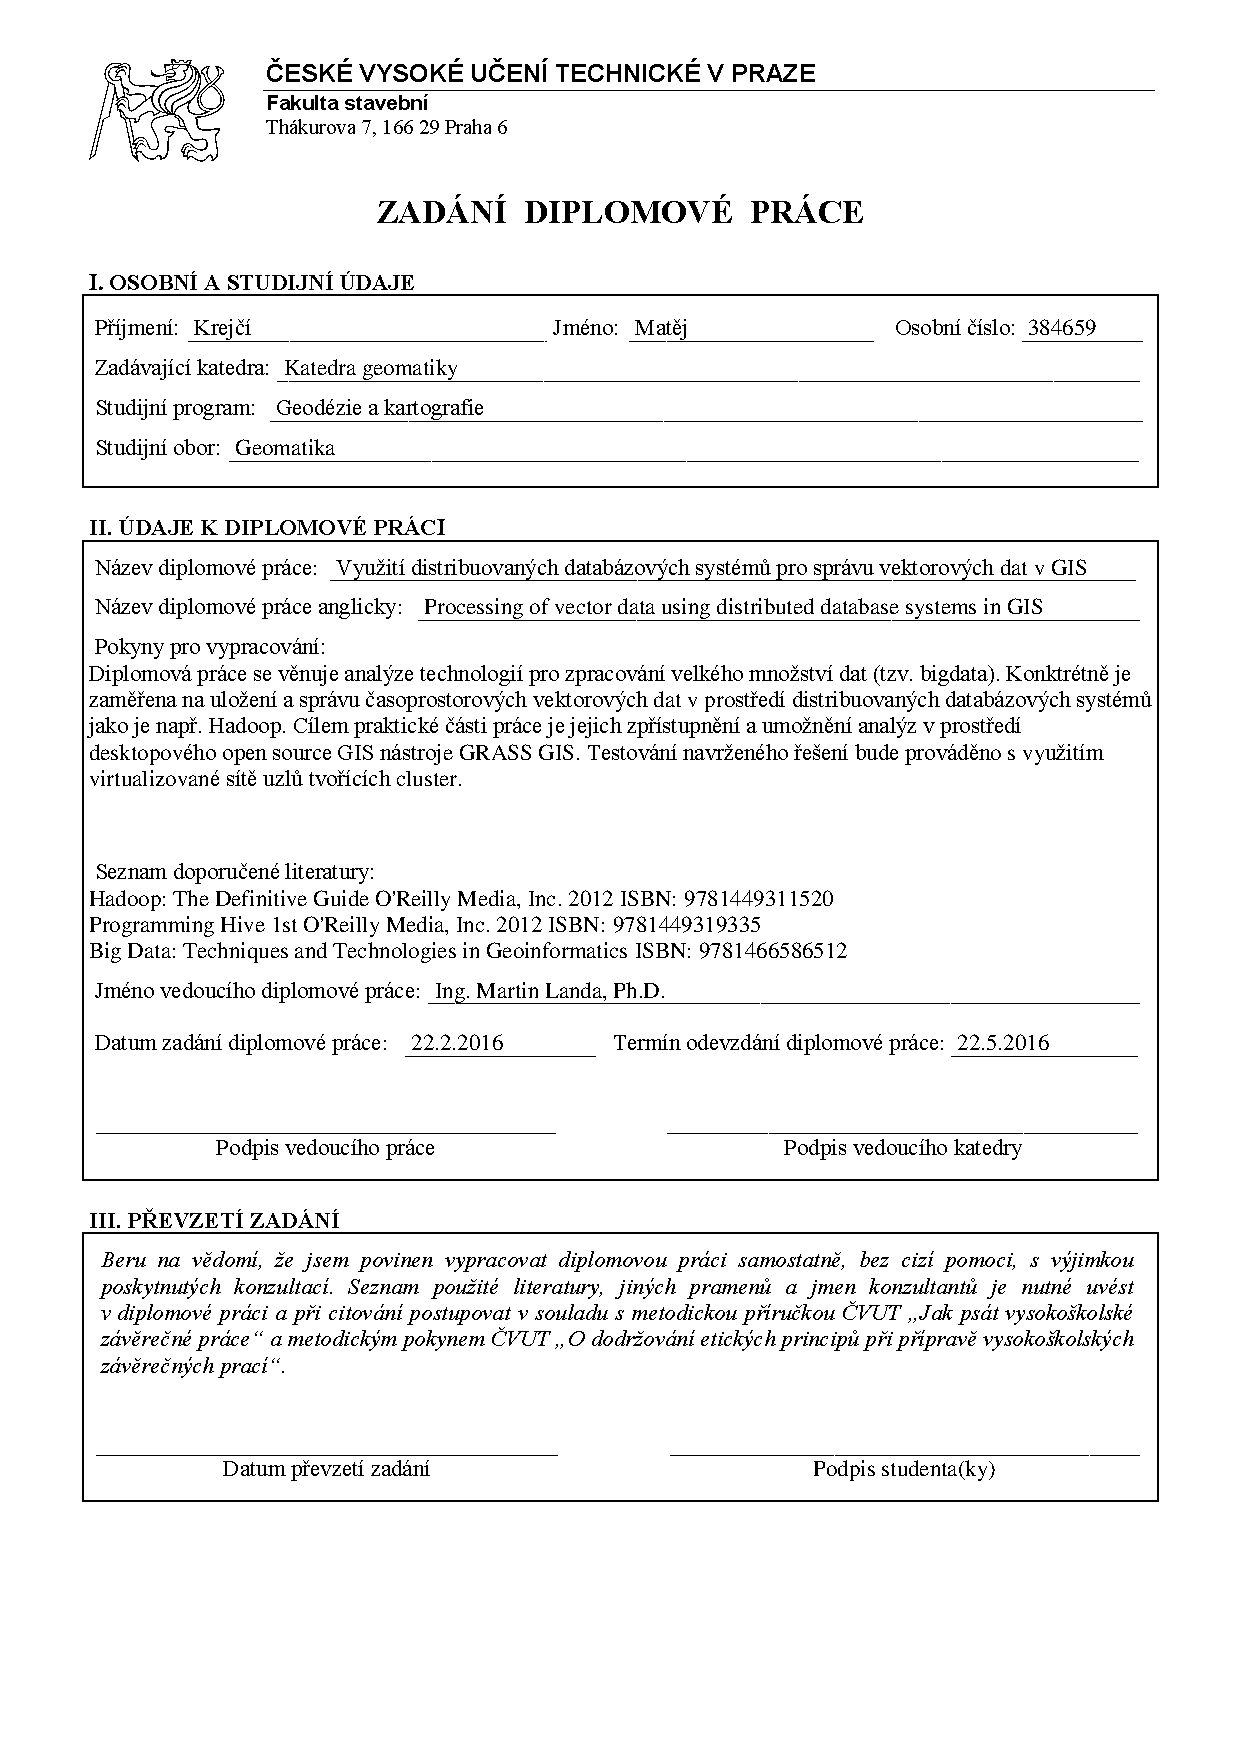
\includepdf[picturecommand={\put(100,200){\vlozZadani}}]{../zadani/zadanidp.pdf}

	\newpage
	\begin{abstractpage}
		\begin{abstractx}{czech}
			
			CIL..
			
			
			\klicslova{Klíčová slova}{GIS, GRASS}
		\end{abstractx}
		
		\begin{abstractx}{english}
			
			Aim of...
			
			\klicslova{Keywords}{GIS, GRASS}
		\end{abstractx}
	\end{abstractpage}
	
	

	
	\newpage
	\newcommand{\odsaditodzhora}{\hskip1pt\vfill}

\odsaditodzhora
\noindent {\bf Declaration of authorship}

\vskip 1.5 \baselineskip

I declare that the work presented here is, to the best of my knowledge and
belief, original and the result of my own investigations, except as acknowledged.
Formulations and ideas taken from other sources are cited as such.

\begin{flushleft}
\begin{tabular}{cp{0.3\textwidth}c}
In Prague .................
& 
&
..................................
\\
&&
(author sign)
\end{tabular}

\end{flushleft}
\newpage

\odsaditodzhora
\noindent {\bf Acknowledgment}

\vskip 1.5 \baselineskip

I would like to thank my parents for their support during my studies.
Great gratitude, I would like to express Martin Landa, my supervisor, for giving sense to my university studies.
\newpage

	\newpage
	
	\setcounter{tocdepth}{3}
	
	\tableofcontents
	%\addtocontents{toc}{~\vspace{-3\baselineskip}}
	
	
	\newpage
	\necislovana{Introduction}
	
	\pagestyle{fancy}
	\fancyhf{}
	\renewcommand{\sectionmark}[1]{\markboth{#1}{}} % set the \leftmark
	\fancyhead[L]{CTU in Prague}
	\fancyhead[R]{\leftmark} % 1. sectionname
	\fancyfoot[C]{\thepage}
	
	
	\pagenumbering{arabic}
	\setcounter{page}{1}
	\subsection*{Context}
%%% JK:capability nebo capacity	
%%% MK:ok
	Over the years, the capacity of hard drives have increased massively and
	access speed too. According to the study undertaken
	by International Data Corp, since 2007
	we produce more data than we can store. Furthermore, the generators of data 
	growing fast which is proofed by the fact that 90\% of data volume has been
	generated since 2010. Current  annual global data production is  7.9 zettabytes
	and the trend points 35 zettabytes in 2020 due to 30 times faster generation of
	data\cite{digit_universe}. 
	The term \textit{big data} became as widely used expression for the volume of
%%% ML: which are ?
%%% MK: todo
	data which beyond the ability of commonly used software to store and process 
%%% ML: Over years (viz prvni veta odstavce)
%%% MK: ok
	them.   During decades of innovation, SQL relational databases reached limits
%%% JK:decatedes nebo decades
%%% MK:ok	
%%% ML: and closely connected (veta zni divne)
%%% MK: hand by hand
	thank it's architecture design hand by hand with the limitation of
	hardware components.  Software engineering has been naturally pushed to 
	investigate new form for handling big amount of data efficiently.  As  the new
	phenomenon   of storing and managing big data in data centers over the word
	became approach based on distributed file system and parallel computing. At the
	beginning of this stage, big companies developed prototypes of software which
	was strongly dependent on maintenance by top experts from the field.  The
	turning point of the blocker has changed by releasing  Hadoop framework,
	especially after it became a part of Apache project. Since that, many side
	projects based on Hadoop are introduced and together became a synonym of 
	distributed ecosystem. 
	The significant generator of the total data amount are sources of
	spatial data. Geoscience in last decades points strong dependency on
	geographical information systems (GIS). This concept, firstly proposed in 1960,
	gone through  the long process of development, and with increasing computational
	hardware capacity became as the standard  effective tool for user workstations.
	

%%% JK2:
%%% MK:ok	
	With technological improvements in the field of measuring, 
	data are currently captured with higher spatial and temporal resolution. To satisfy requirements of
	efficient data manipulation
	%%% JK: manipulation x handling	, store x storage
	%%% MK:ok	
	, analysis and data storage come out several methods based	expensive high-performance hardware
	 accompanied with technology for parallel
	processing. Several libraries for parallel processing such an MPI or OpenMP and
	Hadoop came with master and node  architecture. The design is built for scaling up a cluster.
	 In contrast to other, Hadoop due to amiable interface for
	developers reflect massive boom of its usage. In the last years, several libraries for raster
	and vector data manipulation and analysis for Hadoop and its
	whole ecosystem of extensions has been developed.	Due to the wide range in clusters
	scalability new room for high-performance computing of spatial data became
	as reality.
	
	
	\subsection*{Motivation}
	Several spatial frameworks for Hadoop has been published in last years and
	brings the new 	
	scope of  processing big data in valuable time. Compare to desktop GIS tools
	which are suited for users with different scale of experience, Hadoop
	environment, its configuration, deployment and usage of MapReduce is still
	challenging task. Effective storing of data expressive control is ensured by developed spatial
	frameworks, where the  main functionality can be controlled within the extension such Hive or Pig. 
	Thus more expressive way of interaction is supported and like-SQL
	approach on the top of Hadoop is provided. 
	
	The workflow of processing spatial data using  Hadoop and its spatial libraries
	consists several steps, such as configuration cluster, configuration Hadoop,
	network and security configuration, exporting spatial data to serialization
	format, transferring data to the cluster and distributed filesystem, knowledge
	of Hive data warehouse, querying data using spatial framework, and  finally
	exporting and visualization of the result in GIS. Non automated processing cost time, and
%%% ML: posledni veta?
%%% MK: ok
	without well designed process workflow is not effective.
	
	
	\subsection*{The Aim and Contribution}
	The main motivation of the work is to develop framework which simplify the
	process workflow. 
	
	Generally, to get familiar with the background of technology,
	select of appropriate components and develop tools which simplify each step as is
	possible. 
%%% JK as?? 
	Thus, the aim is to design effective work flow and developed its
	components for processing big data in valuable time.
	
	The essential task is to deploy cluster. Under the hood of that is
	understanding of Hadoop ecosystem and its configuration. 
	
%%% JK ,to reap the..
%%% MK: ok
	In addition, to utilise the benefits of Hadoop it is suitable to deploy cluster using cloud
	services which ensure fair computation power. Second task of the project, that meet
	requirements of the process simplification, consists of implementation
	of the bridge between Hadoop/Hive systems and environment of GIS. More specifically,
	according to the thesis assignment framework for GRASS GIS (free open source geo-spatial framework) is implemented. 
%%% JK	posledni veta nema sloveso
%%% MK: ok	

	
	
	\newpage
	\chapter*{Background of Related Work}\stepcounter{chapter}\addcontentsline{toc}{chapter}{Background of Related Work}
	The chapter \textit{Background of related work} is focused on familiarization
	with theoretical aspects which are essential for fulfilling the aim of the work.
	Firstly, introduce the Hadoop system, which supports distributed filesystem for
%%% ML: or YARN
%%% MK: ok footneote
	manipulation with data and computational framework MapReduce \footnote{MapReduce version 2 is also called YARN} for
	parallel processing. 
	The next section is focused on review and comparison of spatial frameworks for
	Hadoop which support geoprocessing tools of big data. For fulfilling the
%%% ML: libraries?
%%% MK: ok
	capacity of Hadoop and its extensions is essential to dispose cluster of computer
	machines. Thus, the last  part of theoretical introduction is aimed on cloud
	services and its challenges.
	\section{Hadoop Framework}
	\label{sec:hadoop}
	\subsection*{Hadoop}
	\emph{"The Apache Hadoop software library is a framework that allows for the
		distributed
		processing of large data sets across clusters of computers using simple
		programming 
		models. It is designed to scale up from single servers to 
		thousands of machines, each offering local computation and storage. Rather
		than rely 
		on hardware to deliver high-availability, the library itself is
		designed to detect and handle failures at the application layer, so
		delivering a 
		highly-available service on top of a cluster of computers,
		each of which may be prone to failures."}(Apache Hadoop,\cite{hadoop_web})
	\begin{figure}[!htbp]
		\centering
		
\includegraphics[width=0.3\textwidth]{./img/664px-Hadoop_logo.png}
		\caption[Hadoop architecture2]{\centering Hadoop Logo.}
	\end{figure}
	
%%% ML: chybejici reference
%%% MK: ok
	\paragraph*{History} of Hadoop started in 2007 but the roots go
	to Apache Nutch project. 
	
	At the beginning of October 2003, Apache Nutch\cite{nutch_web} has been lunched.
	Apache Nutch is a  web search engine. In the short time (in January 2006) was
	moved to the new Hadoop sub project.
	At the same time  distributed filesystem called Google
	filesystem\cite{google_fs}, with the specific, permitting, efficient and
	reliable access	to the huge amount of data, has been created. This abstract filesystem, widely
	called "user level"~filesystem, runs as a service that is accessible via APIs and libraries. 
%%% ML: Neplatna reference
%%% MK: ok
	In 2008, Hadoop made own top-level project at Apache.\cite{hadoop_news_web}
	By this time, Hadoop was being used by many
	other companies besides Yahoo!, such as Last.fm, Facebook, and the New York
	Times. 
	
%%% ML: zdroj obrazku (pokud vlastni prace, tak uvest)
%%% MK: moje
	\begin{figure}[!htbp]
		\centering
		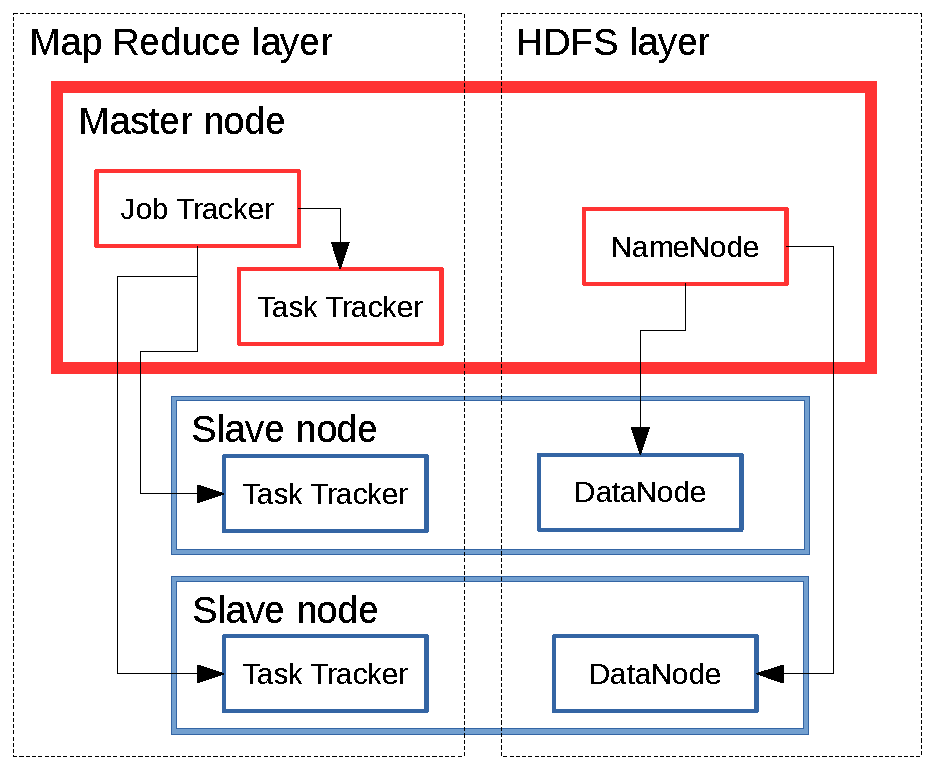
\includegraphics[width=0.6\textwidth]{./img/schema2.pdf}
		\caption[Hadoop architecture2]{\centering Hadoop HDFS and MapReduce layers. Fig. author Matej Krejci}
	\end{figure} 
	
	
	
	\paragraph*{The base Apache Hadoop}framework written in Java is composed of the
	following modules (Hadoop Apache \cite{hadoop_web}):
	\begin{itemize}
		\item \textbf{Hadoop Common} - The common utilities that support the other
		Hadoop modules;
		\item \textbf{Hadoop Distributed File System (HDFS)} – A distributed filesystem
		that provides
		high-throughput access to application data;
		\item \textbf{Hadoop YARN} - A framework for job scheduling and cluster resource
		management;
%%% ML: viz http://hadoop.apache.org/
%%% MK: ok
		\item \textbf{Hadoop MapReduce} - an implementation of the MapReduce programming
		model 
		for large scale data processing. Since version 2 the MapReduce is YARN-based system
		 for parallel processing of large data sets.
	\end{itemize}
	All the modules in Hadoop are designed with an expectation that hardware failures
	are common and thus 
	must be automatically managed by the architecture of  software.
	
	The Hadoop framework is written in Java with some native code in C and command
	line utilities written 
	as shell-scripts. Moreover, for development \textit{Map} and \textit{Reduce}
	parts  
	with using "Hadoop Streaming" any programming language can be apply. 
	Beside main modules, there are many Hadoop extensions for cluster management,
%%% ML: this theses ?
	data access and helpers for storing data in HDFS. As suitable example for using spatial libraries is Apache Hive, 
%%% ML: SQL-like ?
%%% MK: ok
	which expose higher level user interfaces and provide SQL-like query syntax. 
	
%%% ML: in the core ?
%%% MK: ok
	
	There are two main components of the Apache Hadoop 1.x: (1) the Hadoop
	Distributed File System 
	(HDFS) and (2) the MapReduce parallel processing framework. 	
	For Hadoop 2.x have been developed new MapReduce 
	framework named YARN, which handle better the week point of MapReduce v.1.
	
	
	\subsection{HDFS: Hadoop Distributed File System}\label{subsec:hdfs}
	As the main source for describing HDFS is used the official documentation
	(\textit{hadoop.apache.org} 
	\cite{hadoop_web}) and  \textit{Hadoop: The Definitive
		Guide}\cite{hadoop_definitive}
	
	\paragraph*{Hadoop} comes with a filesystem and since it manages the storage of
	files on several 
	machines, it is called Hadoop Distributed filesystem (HDFS). 
%%% JK: 
%%% MK: ok	
	HDFS is designed for handling very large files with streaming
	data access. As example suits well CSV, JSON or any data structure which can be
	serialized. \cite{hadoop_hdfs_web} In HDFS, large files are broken down into
	smaller blocks (128MB, by default) which are 
	stored as independent units. The architecture of HDFS is a highly fault-tolerant
%%% ML: permeability
%%% MK: ok - propustnost
	and provides high permeability for access.   
	A short overview of main characteristics of HDFS design is described in
	(Hadoop: The Definitive 
	Guide\cite{hadoop_definitive}) as five features: \textbf{Very large files} -
	With relevant hardware data of amounts petabytes 
	can be accessed on Hadoop clusters effectively. \textbf{Streaming data access} -
	Efficient data processing is based on
	read once and copied many times pattern. \textbf{Commodity hardware} is
	suitable for running Hadoop. At the end,
	this fact helped with the decision to invest value of money to the development
	of Hadoop instead 
	of operating on expensive and highly reliable hardware. \textbf{Low-latency
		data access} - HDFS is not suitable for performing
	low-latency access to data. Primary, HDFS is optimized for delivering
	a high throughput of data. \textbf{Lots of small files} allows to read and
	operate over more files
	at the same time. Limitation of number of stored directories,  files and block
	in filesystem is limited by \emph{NameNode} memory.
	
	HDFS is based on traditional hierarchical file model. As in other filesystems,
	HDFS allows basic file operations: 
	read, write, rename, move etc. However it doesn’t support hard and soft links. 
	
	\begin{footnotesize}
		\begin{lstlisting}[style=mybash]
#copy file in distributed file system
$ hadoop fs -cp /user/hadoop/file1.csv /user/tmp/file1.csv 
		\end{lstlisting}
	\end{footnotesize} 
	The example above shown copying file between HDFS folders. 
	
	
	\subsubsection{Organization of Data}
	Similarly to  a common filesystem, HDFS is based on the disk blocks as well. The
	traditional
	filesystem is based on blocks which define the minimal size of the amount of
	data to read and write.
	HDFS blocks have the similar concept based on blocks, but the minimal unit is
	larger. The size of the block is 128 MB by default. Blocks are broken and
	distributed
	over disks on the cluster like blocks over a single disk in the filesystem. The
	ideal 
	size of stored files is the same as the size of the block. With increasing the
	block 
	size time cost for computing increases as well. On the other hand, a large
	number
	of blocks is expensive for the preparation of files. The important task is to
	find the optimized 
	ratio between the data preparation and the computational time by setting suitable
	blocks size.
%%% JK:		 by set??
%%% MK: ok
	The idea of block abstraction helps to bring several benefits.
%%% JK:	 První výhody 
	The abstraction design allows to store larger file than the physical disk
	unit, 
	even the fact that for Hadoop it is unusual.
	
	The second benefit of fixed size is simplifying storage management. Even file
	size not fully 		
	fills the filesystem block, the block is not use for other files. 
	Obviously, it makes easy 
	to hold calculating of size discernibility and eliminating metadata concerns
	(not necessary 
	to store metadata of tree in data blocks, even in the same system)
	Furthermore, the blocks are suitable for replication and for providing fault
	tolerance. Protection
	against corrupted blocks, disks or machines is based on replication of block
	over a cluster. 
	Moreover, this approach ensures the integrity of HDFS checksums when writing as
	well as reading data.
	
	\textbf{Replication selection process} is suited to minimize bandwidth
	consumption over a cluster. 
	To minimize read latency, HDFS is primary try to read the closest replica to the
	reader. Priority is the 
	same for rack as for node reader. \cite{hadoop_hdfs_web}
	
	\textbf{Rack Awareness} on Hadoop serves the maximum potential of production, 
	it means that it knows the network topology. The purpose of rack-aware
	replication is ensured by policy 
	component. It controls data reliability, availability, and network bandwidth.
	For a multi-rack cluster it is suitable to map and link
	nodes to a rack\cite{hadoop_rack_web}. This can be ensured manually or using
	program for mapping hierarchy of IP 
	addresses. The priority of transfers is a size of bandwidth availability. Within
	transfers 
	where there is more bandwidth available as compared to off-rack transfers for
	MapReduce jobs on a node. 
	By theory, the better network bandwidth is between machines in the same rack,
	due to hardware specifics.
	
	\subsection{Hadoop Server Components}
	Machines for Hadoop deployment count several server components such as Master
	Servers and Slave Servers and for the access Client Machines.  Hadoop consists
	five main components: 
	\begin{itemize}[noitemsep]
		\item NameNode
		\item DataNode
		\item Secondary NameNode
		\item JobTracker
		\item TaskTracker
	\end{itemize}
	These are basically daemons or programs that run on different physical servers.
	The figure \ref{hdfs_arch} describes the main components and connections
	between them.
	
	\paragraph{Client}
	computers have installed Hadoop with  all the configuration but they are not
	hosted on Master or Slave 
	server. The Clients task is to  load data into the cluster, submit jobs and get
	the result or looking for jobs when finished.
	
	\subsubsection{NameNode, DataNode and SecondaryNameNode}
	Hadoop comes with cluster architecture based on master (\textit{NameNode}) and
	slave (\textit{DataNode}) design pattern. 
	The \textit{NameNode} handles metadata of abstract filesystem (namespace), which
	include
	information about the structure of files and directories in the tree.  It does
	not hold any cluster data itself. 
	The  \textit{NameNode} only knows blocks which make up a file and where those
	blocks are located in the cluster.
	Information about filesystem is stored on local disk in two files: the namespace
	image and edit log file. 
	The \textit{NameNode} knows all locations of  \textit{DataNodes} blocks where
	data 
	are stored. It also provides the primary user interface to access HDFS. 
	By design \textit{NameNode}  is a single point of failure and should be never
	overloaded and must 
	be the most reliable node of the cluster.  Without \textit{NameNode}, HDFS is
	totally unserviceable. 
	\begin{figure}[!htbp]
		\centering
		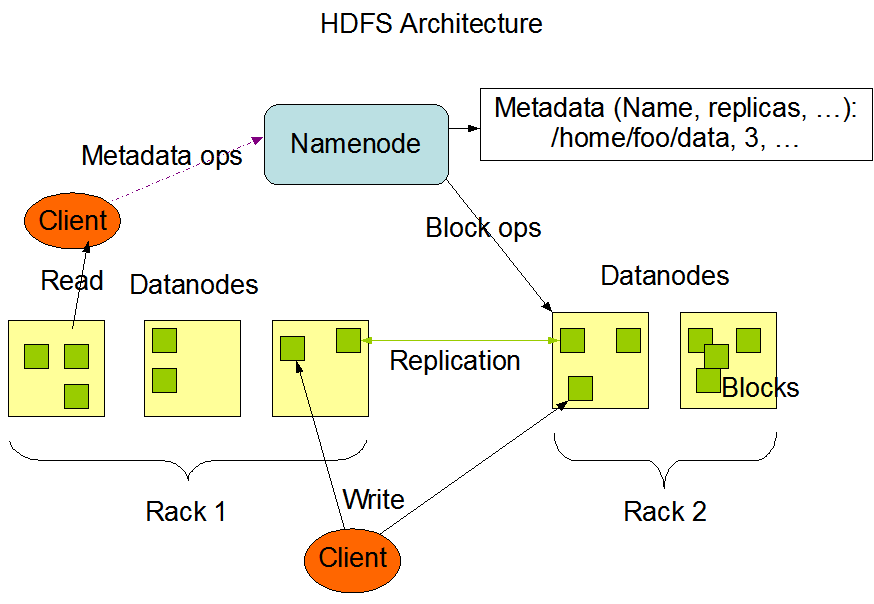
\includegraphics[width=0.8\textwidth]{./img/hdfsarchitecture.png}
		\caption[HDFS architecture1]{\centering HDFS architecture \footnotemark}
		\label{hdfs_arch}
	\end{figure} 
	\footnotetext{Figure source:
		\url{https://hadoop.apache.org/docs/r1.2.1/hdfs_design.html}}
	In recent Hadoop releases, there is also a backup node -
	\textit{SecondaryNameNode}, always up to date 
	with latest (per 1 hour by default) \textit{NameNode} status. It receives all the
	operations done by \textit{NameNode} and 
	stores them in local memory. This permits to have the latest, up to date
	namespace status, when \textit{NameNode} fails. 
	
	As has been mentioned, the blocks of a file are independently stored in nodes,
	which are called
	\textit{DataNodes}. Each \textit{DataNode} in the cluster makes registration
	process to the \textit{NameNode} during start. 
	Besides that, each \textit{DataNode} informs \textit{NameNode} about blocks
	availability by sending a block report. 
	Block reports are sent periodically or when a change event happens. Moreover,
	every \textit{DataNode} sends 
	\emph{relevant} messages to the \textit{NameNode} to confirm that
	it remains operational and that the data is safe and available. If a
	\textit{DataNode} stops operating, the error 
	mechanisms designed to defend the failure and data loss maintain the
	availability of the block.
	\emph{Relevant} messages also hold information, which allows \textit{NameNode}
	to run the cluster efficiently e.g. 
	load balancing. One important concept of design  is that \textit{NameNode} never
	directly calls data.
	
	
	\subsubsection{JobTracker and TaskTracker}
	Above the filesystems is  the MapReduce layer, in other words, MapReduce engine,
	which consists of 
	JobTracker,  which ensures client applications to submit Map\-Reduce jobs. The
	JobTracker handle work 
	out to available TaskTracker nodes in the cluster, 
	aiming to keep the jobs close to a data block.  Thus, JobTracker and TaskTracker
	are two types of 
	nodes for managing the execution process of  task.
	Client submits MapReduce job  to the JobTracker to process a particular file.
	JobTracker choose the 
	DataNodes which store block with the desired file by asking the NameNode where 
	metadata of filesystem are stored. 
	JobTracker appends tasks to TaskTracker according to the  information obtained
	from NameNode and monitors the status of each task.
	
	
	\subsection{HDFS access} 
	Several ways how to use HDFS interactively are available. In analogy to
	filesystem, the main task is manipulation with data, access rules and additional
	to load data to distributed filesystem. As in standard filesystem, the permission model is
	provided in HDFS as well. 
	In paragraphs below there are described accesses  HDFS 	
	methods and permission models.
	
	\paragraph{Permission model}
	The permission model of HDFS has several levels. The level of files and
	directory is similar to POSIX model. 
%%% JK co je posix (operating system functionality in a C language interface)	
	Each file and directory are associated with
	an owner and a group. Each item in HDFS, such a file and directory, has separate
	permission. Thus, individual permissions for the user, for other users that are
	member of group and the rest of users can be assigned. 
	Permission is \textit{r} for reading,
%%% JK:	Permission are:
	\textit{w} for writing and \textit{x} not for execution, but for permission to
	access a child of the directory.\cite{permission}
	
	There are two different models for checking the user's identity.
	\begin{itemize}
		\item \textbf{Simple}  In this model is an identity of user derived from host
		operating system.
		\item \textbf{Kerberos} In Kerberos model, the identification process is managed
		by 'tickets' based on Kerberos credentials system which allow nodes communication
		over a non-secure network to prove their identity to one another in a secure
		manner.\cite{kerberos}
	\end{itemize}
	
	The identity mechanisms are  extrinsic to HDFS itself. Thus, within HDFS there is no
	handler for creating user identities, establishing groups, or processing user
	credentials.
	
	\paragraph{Access mechanisms}
	The basic mechanism for interaction with HDFS is \textit{hadoop fs}  command
	line tool \textit{bin/hadoop fs $<$args$>$}. 
	All fs shell commands take path URIs as arguments. Most of the commands in fs
	shell are derived from Unix commands. 
	
	The other mechanism for accessing HDFS is through application programming
	interfaces such a APIs: Native Java API, which has a base class
	\textit{org.apache.hadoop.fs\\.FileSystem}; C API that works through the
	\textit{libHDFS} library, and there's a header file, \textit{hdfs.h} which has
	information on the API calls.
	
	In addition, interaction according standard REST API is available. REST API is
	an architectural style consisting set of rules and constraints applied to
	components within distributed systems. The WebHDFS REST API components fully
	cover the standard fs tool. The API consists four main groups of HTTP requests,
	such as: HTTP GET for fetching information, HTTP PUT for manipulation request,
	HTTP POST for append or concat file and HTTP DELETE for deleting files and
	directories.\cite{rest_api}
	The Unix tool \textit{curl}  allows accessing API from the Unix terminal. 
	\begin{footnotesize}
		\begin{lstlisting}[style=mybash]
$ curl -i -X POST -T <LOCAL_FILE> "http://<DATANODE>:<PORT>/webhdfs/v1/<P..."
....

HTTP/1.1 200 OK
Content-Length: 0
		\end{lstlisting}
	\end{footnotesize}
	The example above demonstrates submit  HTTP POST request using the URL in the
	Location header with the file data to be appended. The client receives a
	response with zero content length.
	
	
	\subsection{Parallel computing - MapReduce}		
	The \emph{MapReduce} is a programming model for processing and generating large
	data
	sets. The \emph{MapReduce} abstraction is inspired by the Map and Reduce
	functions, which are commonly
	found in functional programming languages, such as LISP \cite{lisp}. Users can
	easily express their
	computation as a series of Map and Reduce functions. The Map function processes
	a series of
	\textit{$<$ key, value $>$} pairs to generate a set of intermediate \textit{$<$
		key, value $>$} pairs.
	\begin{center}
		Map(keyA, valueA) → list (keyB, valueB)
	\end{center}
	Reduce function aggregates all intermediate values that associate to the same
	intermediate key
	to produce the final output, also in the form of $<$ key, value $>$ pairs
	\begin{center}
		Reduce(keyB, list(valueB)) → list (key C, valueC)
	\end{center}
	Thus the \emph{MapReduce} framework transforms a list of (key, value) pairs into
	a list of values. 
	
	
	\paragraph{As MapReduce demonstration} the data from cellular microwaves
	links (MWL) are used.
	After  the data are  serialized and stored in text files each file
	represents captured data for 24 hours time interval. 
	The size amount of weakly data is relatively small (100Mb)
	which suits well to the default block size(128Mb).
	The aim is to compute  mean of differences between transmitted and received
	signal for each link in the period between 2014-07-07 and 2015-07-07.
	
	Below is the sample of data stored as CSV.
	\begin{footnotesize}
		\begin{lstlisting}[style=mybash]
linkid;data;rx;tx
324;"2014-07-07 11:14:56.552";-48.9;10
256;"2014-07-07 11:14:59.703";-99.9;7
...
324;"2015-07-07 17:10:56.578";-50.1;7;
256;"2015-07-07 17:10:56.484";-85.3;10;
		\end{lstlisting}
	\end{footnotesize}
	The text lines above are presented to map functions as key-values pairs.
	The map function extracts data from date 2014-07-07 and creates pairs
	{link:(rx-tx)}
	\begin{footnotesize}
		\begin{lstlisting}[style=mybash]
{324:-58.9}
{256:-106.9}
...
{324:-57.1}
{256:-95.3}
		\end{lstlisting}
	\end{footnotesize}
	The output is processed by MapReduce framework before is being sent to reduce
	function.
	Mentioned process sorts pairs by key as shown bellow.
	\begin{footnotesize}
		\begin{lstlisting}[style=mybash]
{324:[-58.9,-57.1]}
{256:[-106.9,-95.3]}
		\end{lstlisting}\end{footnotesize}
	Finally reduce program iterates over the list of values for each link and
	compute mean.
	The final results are stored in Hadoop filesystem.

	
	\section{Spatial Processing in Parallel}
	\subsubsection{Introduction to Spatial MapReduce Query}
	Figure \ref{fig:mapred_spatial} shows a simple example of distributed spatial
	query processing. The main idea 
	grows up from the basis of MapReduce. On the figure, the dataset is partitioned
	into four tiles. After 
	query job is started, each tile is analyzed separately using Map (M1-M4)
	function. For demonstration, 
	query analyzes intersection of two datasets (red, blue) on each tile. Thus,
	relation between 
	objects from the different dataset is detected. The result is done by Reduce (R)
	function, where results from each
	map phase are processed.
	
	\begin{figure}[h!]
		\centering
		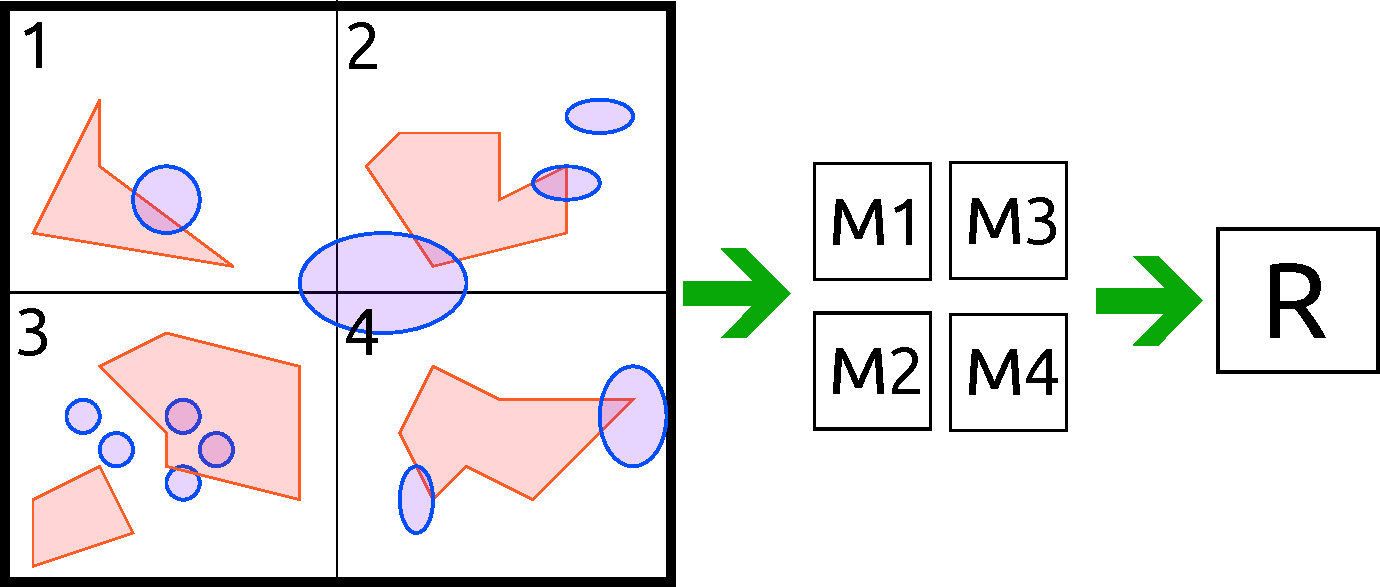
\includegraphics[width=0.6\textwidth]{./img/mapred_spatial.pdf}
		\caption[Spatial MapReduce]{\centering Detection of spatial relations using
			Map (\textit{M1-M4}) and Reduce (\textit{R}) functions}
		\label{fig:mapred_spatial}
	\end{figure}
	\paragraph{}
	
	The motivation for spatial processing in parallel is querying data in reasonable
	time. 
	Firstly, it is essential to introduce characteristics of queries for solving
	different 
	tasks. In HadoopGIS (F. Aji, F. Wang, et al.\cite{hadoopGIS})  five major 
	query cases of spatial data is defined: (1) \textit{Feature Aggregation queries}
	which doesn’t 
	fall into spatial queries, however, they are evenly important for spatial
	frameworks 
	as others. As a common example of Feature Aggregation query, a function for
	finding mean 
	values of attributes. 
	(2) \textit{Fundamental Spatial Queries} covers groups of tasks like: including
	point based 
	queries, containment queries, and spatial joins. (3) Next groups 
	\textit{ Complex Spatial Queries} includes more challenging task. A query which
	solves 
	advanced Spatial Join: spatial mismatching or overlay; or neighbor query. (4)
	Integrated 
	spatial and feature queries, which combine query from more categories, such
	feature 
	aggregation queries in a selected spatial regions. Finally (5) \textit{Global
		Spatial Pattern Queries}, for example, queries on finding high-density regions,
	or 
	queries to find directional patterns of spatial objects.
	
	Anyway, classification of a query to five groups is based on characteristics of
	a task. 
	But, as in RDBMS and also in distributed databases, the most challenging is to
	solve  cost-intensive query. 
	Join Queries and Nearest Neighbour queries can be classified as 
	cost-intensive to compare to the rest. That fact points these query as the
	interesting and
	most challenging task for a scientist and developers. Naturally it affects the
	direction of the most of academic works and developments.
	
	Speeding up a process of solving \textit{Spatial Join} which is classified as
	classic GIS 
	problem is a motivation for the parallel processing of spatial data. Spatial
	Join 
	is an operation used to combine two or more datasets with respect to a spatial 
	relationship. Detection of relations between spatial objects using serial (used
	in RDBMS) 
	computing approach started to be limited by its design. On the scene comes
	solutions
	based on parallel and distributed models. In the past, many distributed 
	solutions as OpenMP\cite{omp} have been presented, for instance, Intel TBB and
	Bulk Synchronous Parallel\cite{multi_cpu}.
	Because of their complexity, they have been used insignificantly to compare with
	Hadoop framework.
	Already introduced MapReduce parallel model opens doors for developing efficient
	spatial query engine with less developing investments. In the last years,
	several Spatial MapReduce projects came up on the scene.
	\textit{SpatialHadoop}\cite{spatialhadoop}, \textit{HadoopGIS}\cite{hadoopGIS}
	and \textit{ESRI Spatial Framework for Hadoop}\cite{ESRI_framework}
	are three open source libraries that are designed to process large scale spatial
	data within the integration of Hadoop.
	All three systems come with significantly different design of implementation but
	they all are based
	on MapReduce framework from Hadoop environment and basically all project have
	the same goal.
	To realize such systems, it is essential to identify time-consuming spatial
	query components,
	break them down into small tasks, and process these tasks in parallel. 
	Design of the first two systems, \textit{SpatialHadoop} and \textit{HadoopGIS}
	extensions are well described in publications. Back\-ground of ESRI library is not
	described in an available
	literature, on the other hand, the user documentation seems to be complex and
	described in detail. 
	ESRI laboratory published article\cite{ESRI_indexing} about QuadTree indexing,
	which is used for building 
	indexes in their \textit{ESRI Spatial Framework for Hadoop}.
	In the section below are described fundamentals of spatial processing in
	parallel and  discussed 
	the comparison of solutions of developed and published frameworks is provided.
	The main source for features analyses of spatial frameworks design are already
	mentioned literature sources (\textit{SpatialHadoop}\cite{spatialhadoop},
	\textit{HadoopGIS}\cite{hadoopGIS} 
	and \textit{ESRI Spatial Framework for Hadoop}\cite{ESRI_framework}).
	
	
	\subsection{Spatial Join}
	\label{sub:spatial_join}
	Assume two sets of multi-dimensional object in \emph{Euclidean space}. 
%%%JK: Spatial join relation betw... 
%TODO
	Relation of spatial join between sets \emph{R} and \emph{S} can be defined\cite{spatial_join2}:
	
	\begin{center}
		$R\bowtie_{pred}S=\left \{ \left ( r,s|r  \right )\in R,s \in S, pred(r,s) is \
		\ true) \right \}  $
	\end{center}
	where $\bowtie_{pred}$ is a spatial predicate for the relationship of two
	spatial objects. 
	\linebreak 
	\textit{Spatial join} finds all pairs of object which satisfying a spatial
	relation between given objects. 
	For further explanation of the spatial join concept assume that  objects
	\emph{s} from set \emph{S} and 
	analogically  \emph{r} from \emph{R} are rectangles. Intersection operation
	between each rectangle \emph{s} 
	and \emph{r} will report set \emph{R} of intersected \emph{r} rectangles.
	
	Solution of described \textit{spatial join} is trivial. General spatial join
	problem has been extended by 
	complex spatial join, known as \textit{spatial overlay join}\cite{spatial_join}:
	(a) The set of objects
	can be another character than a rectangle, such as point, segments or polygon.
	(b) The dimension of a set 
	can be more than three. (c) The relationship between pairs of objects may be any
	relationship between 
	objects which includes spatial elements, such as intersections, nearness,
	enclosure, or a directional relation. 

	To speed up spatial join query different ways based on filtering are commonly
	used.
	Typical trivial solutions are reached by usage of Minimal Bounding Box (MBB) as
	a first 
	filter for defining the subset of candidate object satisfying a spatial
	predicate. For defining MBBs for 
	sets of points Convex Hull algorithm can be used. 
	To speed up construction computation  of Convex Hull based on heuristic
	\cite{covex_hull} is more efficient. 
	In Spatial Join technique \cite{spatial_join}  different methods of  spatial
	objects filtering according the specific requirements are used. For large
	dataset stored in GIS, the filtering is essential. Objects such a polygon 
	or point cloud can reach millions or more features. Boolean vectors operation on
	detecting relation without filter stage 
	can be extremely expensive in a meaning of I/O performance. Usually, in the
	first stage there is filtering data; spatial objects 
	are read from hard drive which is sufficient for computation of MBRs, then
	created MBRs are 
	stored in memory and the spatial join test is performed faster.
	
	
	\subsubsection{Spatial Partitioning}
	\label{Spatial_Data_Partitioning}
	Data partitioning is a powerful mechanism for improving an efficiency of data
	management systems, 
	and it is a standard attribute in modern database systems. Partitioning data
	into smaller units provide room for query processing in parallel and further
	improved performance. In addition,
	with proper partition scheme, I/O operations may be substantially
	reduced by scanning only a few sections that contain relevant information to
	answer a question.
	Within the architecture of Hadoop, the important step and the first one is defining a
	suitable format for 
	storing data which influences  speed of their access and query execution.
	In general,
	partitioning produces sub-datasets based in smaller regions-tile.
	There are two main reasons for the partitioning of spatial data. 
	The first one is to avoid tiles with high density. This is mainly due to the
	potential high 
	skew\cite{spatial_skew} of data which could imbalance workers in a cluster
	environment. Another aspect is to  
	properly handle boundary of intersecting objects. As MapReduce provides custom
	scheduling  for balancing tasks the problem of load imbalance can be partially 
	mitigated to a task of schedule planning. In work (Effective Spatial Data
	Partitioning for Scalable Query 
	Processing \cite{partitioning}) there has been introduced and compared six methods of
	spatial data partitioning for parallel processing. 
	
	\begin{figure}[h!]
		\centering
		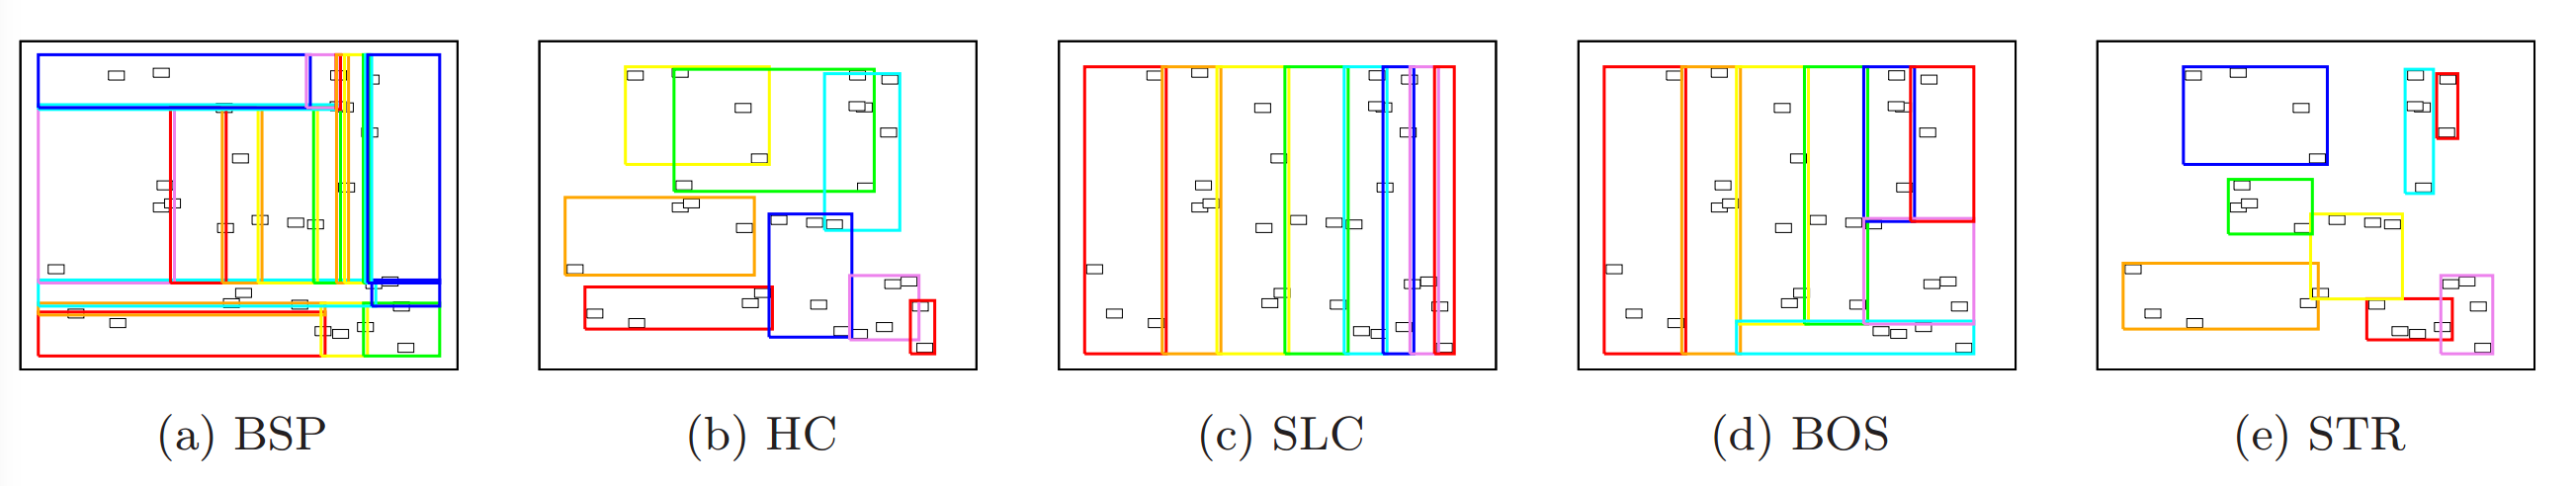
\includegraphics[width=1\textwidth]{./img/part_overview.png}
		\caption[mapreduce flow]{\centering  Spatial partitions generated by
			different algorithms BSP: Binary split 
			partitioning, FG: Fixed grid
			partitioning, SLC: Strip partitioning, BOS: Boundary optimized strip
			partitioning, STR: sort-tile-recursive
			partitioning, HC: Hilbert curve partitioning. Source of fig:
			\cite{partitioning}}
	\end{figure} 
	
	\paragraph{Spatial data skew} is common challenging problem in a spatial
	application. As example \cite{hadoopGIS} assume dataset of 
	$1000\cdot1000$ tiles. The maximum count of the object is $10 000$ objects, but
	the average count is $1020$. This 
	fact growing from the real situation where a high density of objects are e.g. in
	cities and less dense in farmlands. 
	In parallel spatial processing where a distribution of processes is based on
	tiles, the data skew can significantly 
	increase the response time.
	
	\paragraph{Boundary object}
	Spatial partitioning generates boundary objects that cross multiple partitions.
	Thus, it influences the independent relation 
	of each partition. In a usual case, a spatial object has complex boundary and
	extent. Even more, 
	from real experience is evident that in spatial datasets object can cross
	multiple partitions. The problem is solved with 
	different methods; replicating spatial object to multiple partitions and
	filtering duplicates during query process 
	or another approach, creation sectors with putting weight on minimizing boundary
	objects. 
	
	
	\paragraph{} Developed spatial libraries comes with different approaches for
	solving, partitioning, boundary overlay and data skew:
	\begin{itemize}
		\item \textbf{HadoopGIS} in partitioning stage is focused on breaking
		high-density tiles into smaller ones with using 
		recursive partitioning. Firstly, they provide two-dimensional data partitioning
		and generates a set of tiles.
		These preprocessed tiles are a source for query tasks. The preprocessing is done
		with the using of distributed computing.
		Week point of tile-based approach is non-adaptable algorithm on non-uniformly
		distributed data. Because that, 
		critical problem of \textit{data skew} with these spatial partitioning is
		known. \textit{HadoopGIS} ensures 
		this problem by cutting high-density tiles into small ones, thus it use
		recursive partitioning approach. The maximal and a minimal number of objects per
		tile is defined for controlling 
		number of objects per tile . Splitting recursion 
		finds optimal direction(x or y) for creating half-sized tiles which fulfill the
		thresholds by a number of objects 
		in each half.  Taking into account default HDFS blocks size (128MB), the final
		tiles are not stored in small files.
		
		\item  \textbf{SpatialHadoop} implemented the solution  based on the same tiles
		idea as HadoopGIS, but few features 
		are significantly different.
		The main difference is storing partitions (tiles) in HDFS blocks  instead of
		using big batch file. Three main characteristics arise from that fact.
		SpatialHadoop counts 
		a size of HDFS block and the size of tiles should fit that size. It avoids data
		skew of spatial datasets. 
		Secondly, a design of partitioning method ensures spatial locality; a spatially
		close object is assigned to the same 
		partition. The last feature attempts 
		to balancing the size of a partition. In an
		ideal case, all partition are the 
		same size. The number of partitions \emph{n} is computed as $n=S(1+ \alpha)/B$,
		where \emph{S} is the size of input file, \emph{B} is the HDFS block size and
		$\alpha$ is an overhead ratio (0.2 by default). 
		Next step is the definition of boundaries by of partitions. Boundaries are
		represented by rectangles. Thus, a skew of data is not considered. 
		The output of this step is set of rectangles representing  boundaries of
		partition. Together it represents cover 
		of whole space domain. The result is input for initialization of physical
		partitioning procedure. The method solving 
		the problem of an object with spatial extents (e.g. polygon) which overlaps more
		than one partitions. Determination 
		of solution is based on selected indexing method. If some of them assign object
		to all overlapping partitions and 
		the others find the best matching partition. Replicated records are managed
		later by  query processor. Finally, 
		for each record from partition the map function write the pair
		$<$partition,record$>$ which are grouped by 
		partitions and sent to reduce function for the next task- indexing phase.
	\end{itemize}
	
	
	
	\subsubsection{Spatial Indexing}
	\label{Spatial_Indexing}
	One essential requirement for spatial queries is a fast response. 
	In general, the filtering and partitioning  of spatial objects are widely
	related to indexing. 
	Spatial indexing helps to avoid of sequential browsing. In other words to avoid
	full table scanning.
	Generally, in RDBMS for creation index over specified column or multiple columns
	is available multiple 
	indexing methods like btree, hash, gist, and gin. On spatial indexing problem in
	RDBMS have 
	been done many scientific works and different algorithms have been shown.
	Suitability of 
	different indexing methods is linked to the characteristics and distribution of
	data. 
	Adaptation of serial indexing method to parallel processing points non-trivial
	challenge. 
	RDBMS has the ability to use information from multiple indexes to determine how
	best
	to search for the records that satisfy all query criteria. A
	NoSQL key-value store, in contrast, has only a single index.
	That is built atop the constraint that all records are ordered
	lexicographically. Traditional 
	Spatial Indexes from the field of RDBMS e.g. Grid file or R-tree are not
	suitable for parallel 
	processing. 
	
	The architecture of traditional indexing method is not designed for
	effective 	usage on Hadoop, where developers implement indexing in a 
	procedural way and the execution  runs on multiple threads.
	 Since Hadoop is based on MapReduce layer to implement 
	sequential construction instead of incremental one  is necessary.  
	MapReduce is a scan based data processing framework which does not utilize any
	form of a disk-based 
	index and the performance is limited as the input has to be scanned. The design
	of spatial indexing methods 
	must be hand to hand with filtering approach and selected partitioning pattern. 
	
	
	\paragraph{} Developed spatial libraries comes with different approaches that
	solve  spatial indexing challenge:
	\begin{itemize}
		\item \textbf{SpatialHadoop} indexing model is composed from three phases. The
		first phase, partitioning is already described in section \ref{Spatial_Data_Partitioning}.

		The purpose of the second phase is to build \textit{local index}  for each
		physical partition of data. 
		In contrast to global index, the local index is built for each partition
		separately. In addition, each local 
		index is stored in one HDFS block. It ensures that Hadoop uses load balancer for
		relocating blocks 
		across machine. Additionally, it allows  a spatial operation to access local
		indexes where each local 
		index is processed in one map task. 
		
		Last phase, building the \textit{global index} provide index structure of all
		partitions. As next step, 
		all local indexes to one file which represent the final index of spatial data
		are concatenated. This process 
		provides using MapReduce  layer. After this part is done, NameNode creates a
		global index
		and store it in memory. The index is based on dictionary- key and value.
		
		\begin{footnotesize}
			\begin{lstlisting}[style=mybash]
-179.3248215,-54.934357,6.9290401,71.2885321,part-00000_data_00001
-171.773529,-54.81145,6.9261512,65.1480999,part-00000_data_00001_1
6.9225032,-46.44586,179.3801209,78.0657531,part-00000_data_00002_2
			\end{lstlisting}\end{footnotesize}
		
		
		Key is represented by HDFS block and  rectangular boundaries as value. This
		index keeps all the 
		time in the main memory. That ensure faster access. In critic situation when
		fail of master or 
		restart of a cluster is possible to rebuild index from rectangular boundaries of
		the file blocks. 
		For accessing the master index it is not necessary to parse it yourself.
		Implementation offers API 
		which retrieves the global index as an object.
		SpatialHadoop offers tree methods for building indexes. 
		
		The simple one, \textbf{Grid Index} is a flat and partitions of
		data according to a grid such that records overlapping each grid cell are stored
		in one file block 
		as a single partition. Grid index is suitable for uniformly distributed data.
		Otherwise, the data 
		screw is critical by the principle of MapReduce. 
		
		Besides grid index, SpatialHadoop framework offer building index based on method
		\textbf{R-tree} and 
		\textbf{ R+-tree}. Fig \ref{fig:partitioning} (b) shows results of R-tree
		algorithm. 
		
		\begin{figure}[h!]
			\centering
			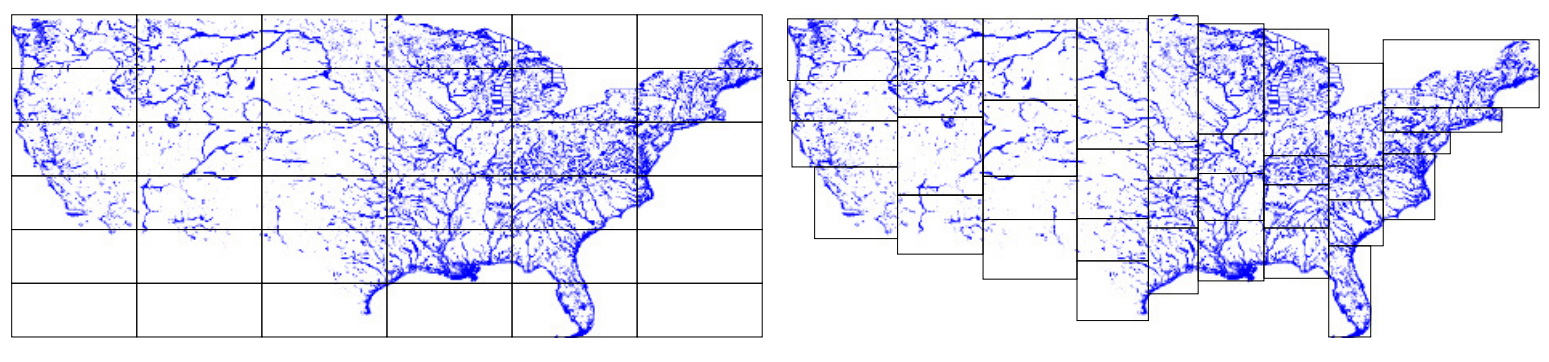
\includegraphics[width=1\textwidth]{./img/spatial_hadoop_parti.png}
			\caption[Spatial MapReduce]{\centering (a) Grid Partitioning (b) R-tree
				Partitioning.\footnotemark}
			\label{fig:partitioning}
		\end{figure}  
		\footnotetext{Source: SpatialHadoop: A MapReduce Framework for Spatial Data;
			Eldawy A., Mokbel,F.M \cite{spatialhadoop} }
		
		\item \textbf{HadoopGIS} indexing is based on hierarchical space partitioning
		and MBB based 
		region filtering. Similarly, the Grid Index design of SpatialHadoop  is built from
		combination of local indexes and global index. Recursively each tile can be further 
		partitioned into even smaller regions. 
		In contrast to SpatialHadoop, HadoopGIS does not pre-generate indexes into
		files. Finally, HadoopGIS supports uniform grid 
		index, which is efficiently applicable only in the rare case of uniform data
		distribution. 
	\end{itemize}
	
	
	
	\subsubsection{Spatial Operations}
	
	
	
	Three mentioned spatial processing frameworks (section \textit{Spatial
		Join}\ref{sub:spatial_join}) 
	for Hadoop show different design for storing and accessing data. Similarly, the
	interface for 
	configuration, data management and query data varies.
	
	Operation on \textit{HadoopGIS} and \textit{ESRI Spatial framework  for Hadoop }
	 are based on like-SQL layer. 
	Particularly on the top of spatial MapReduce library there is implemented  data
	warehouse Hive based on  like SQL commands.
	\textit{SpatialHadoop} supports spatial extension Pigeon a high level SQL-like
	language which  provides OGC-compliant 
	spatial data types and operations making it easier to adopt by users. It makes
	the program simpler and more expressive 
	as it uses spatial data types (e.g. POINT and RECTANGLE) and spatial functions
	(e.g. ST\_Overlaps, ST\_Contain). 
	The implementation of spatial operators are designed to be used as defined
	functions (UDFs) which are seamless to integrate with existing  non-spatial
	operations in Hive or Pig for SpatialHadoop. The spatial operators of all three
	libraries fulfil implementation rules according to OGC standard.
	
	
%%%JK:kontrola velkych/malych pismen v tabulce	
	
		
	\begin{table}[!htbp]
		\begin{footnotesize}
			\centering
			\begin{tabular}{@{}|c||c|c|c|@{}}
				\toprule
				framework    & HadoopGIS   & SpatialHadoop    &
				\begin{tabular}[c]{@{}c@{}}Spatial framework \\ for Hadoop(ESRI)\end{tabular}   
				
				\\ \midrule
				\midrule
				\begin{tabular}[c]{@{}c@{}}integration \\ with extension\end{tabular} & HiveSP  
				&
				\begin{tabular}[c]{@{}c@{}}Pigeon(spatial \\ extension for\\  Apache
					Pig)\end{tabular} & Hive                                                        
				
				\\ \midrule
				\begin{tabular}[c]{@{}c@{}}build-in\\ data types\end{tabular}         &
				\begin{tabular}[c]{@{}c@{}}point, polygon, \\ pox and \\ lineString\end{tabular}
				& \begin{tabular}[c]{@{}c@{}}point, rectangle\\ and polygon\end{tabular}        
				& \begin{tabular}[c]{@{}c@{}}inherit from\\ ESRI Java Geometry \\
					Library: Point, MultiPoint, \\ Polyline, Polygon, Envelope.\\ Also includes OGC
					Wrappers.\end{tabular} \\ \midrule
				input data                                                            & CSV     
				&
				\begin{tabular}[c]{@{}c@{}}CSV,\\ custom \\ data types\end{tabular}             
				& JSON, GeoJSON, text,  WKB                                               
				
				\\ \midrule
				\begin{tabular}[c]{@{}c@{}}user-defined\\ data types\end{tabular}     & -       
				&
				\begin{tabular}[c]{@{}c@{}}- for Pigeon\\ + SpatialHadoop\end{tabular}          
				& -                                                                       
				
				\\ \midrule
				visualisation                                                         & -       
				&
				+*HadoopViz                                                                     
				& \begin{tabular}[c]{@{}c@{}}*Geoprocessing \\ Tools for Hadoop\\
					(ArcMap)\end{tabular}                                                           
				\\ \midrule
				index                                                                 &
				\begin{tabular}[c]{@{}c@{}}uniform grid\\  index\end{tabular}                   
				& R-tree, R+-tree, Grid index & QuadTree                                          
				
				\\ \midrule
				\begin{tabular}[c]{@{}c@{}}accessible\\ index\end{tabular}            & -       
				& +     
				
				& -                                                                             
				
				\\ \bottomrule
				
			\end{tabular}
			\caption{Overview of spatial frameworks for Hadoop}
			\label{tab:comparison_spatial_fr}
		\end{footnotesize}
	\end{table}
	
	\subsection{Summary}\label{summary_libs}
	
	SpatialHadoop, HadoopGIS and ESRI Spatial Framework for Hadoop are
	three open source systems that are designed to process large scale
	spatial data on Hadoop. Although these features of  the implementation of each
	framework are different, 
	the overall design is suited to Map and Reduce function principals. Spatial
	cross join is well suited to parallelizable and fit to MapReduce. 
	
	All three spatial frameworks come with indexing, where SpatialHadoop is the most
	customizable. 
	The design of  SpatialHadoop implementation is open to extending available
	indexes. ESRI and 
	SpatialHadoop offer more advanced indexing methods, such as 
	QuadTree (ESRI) and E-tree (SpatialHadoop). One of the main weakness of HadoopGIS
	is an limited indexing 
	support. It disposes only by grid index method which can be 
	effectively used only for uniformly distributed data.

	To compare with others, SpatialHadoop comes with the different MapReduce
	approach for solving cross-spatial join.
	In SpatialHadoop, both sides in a spatial join are partitioned and 	
	implemented as only 
	Map job.  SpatialHadoop makes pairs from spatially overlapping partitions, which
	are finally 
	assigned to Map tasks for parallel and distributed execution.
	
	In addition, SpatialHadoop implements filtering using MapReduce as a
	preprocessing step.
	HadoopGIS as the first step joins both datasets, reorders and assigns its data to the
	same 
	HDFS block.  Accessing data are provided by key-value pairs. Partitions are
	represented by keys and item as values. 
	
	When decision which framework is suitable for a specific application must be
	made, the 
	key factor can be access of data  or programming language choice. While
	SpatialHadoop 
	uses binary format for representation data in memory and disk, HadoopGIS 
	uses Hadoop streams. Thus, HadoopGIS representing all side results as text and
	access 
	of data is only sequential. In contrast, SpatialHadoop binary approach allows 
	accessing data randomly.
	These facts make SpatialHadoop more efficient since parsing text are an
	expensive task. 
	On the other hand, HadoopGIS allows writing MapReduce function in different
	languages than Java which can be crucial factor. 
	
	
	Generally, all frameworks allow customization on the level of developing
	Map\-Reduce functions. As ESRI 
	framework allows interaction with core libraries, the library is more focused or
	GIS users than developers. 
	ESRI covers the wide portfolio of built-in spatial operators to compare
	SpatialHadoop framework, 
	and at least significantly more than HadoopGIS. On the other hand, the leader
	for customization and 
	development of additional functionality is SpatialHadoop.
	
	
	
	
	\section{Google Cloud Platform}
	\textbf{Cloud} in computer technology means service which provide capability of
	storage and computation engine within datacenter. Services allow to developers 
	work efficiently  with 
	requisite resources which are necessary for an application to work.
	
	\textbf{Google Cloud Platform} supports building, testing and deploying an
	application on highly-scalable infrastructure.
	Developing products using the platform is based on building blocks of particular
	functionality. Advantages of  the platform design is a quick development of 
	desired product by combining separate but compatible services. Portfolio of
	services is parted into six main categories 
	which are overview  in
	table\ref{tab:google_all} \cite{gc_product_services}.
	
	The user interface offers three different ways for managing services of Google
	Cloud. Web-based interface, command-line 
	interface and programming API. With web interface 
	user can quickly get overview and a better understanding of 
	options over each service. On the other hand, the range of configuration
	possibilities is limited compared with the rest 
	interfaces. \textit{Google Cloud SDK} is a 
	package of tools for managing resources and application on Google Cloud
	Platform. 
	Package includes \textit{gcloud} commandline tool for Google Compute Engine
	resources and \textit{gsutil} for working with Cloud Storage.
	
	\begin{table}[!htbp]
		\begin{scriptsize}
			\centering
			\begin{tabular}{@{}|l||l|l|@{}}
				\toprule
				Group                       & Framework                                      
				& Description                                                  
				
				\\ \midrule \midrule
				\multirow{5}{*}{Compute}    & Compute engine                                 
				& large-scale workloads on virtual machines                    
				
				\\ \cmidrule(l){2-3} 
				& Preemptible VMs                                                  &
				short-lived instances for batch and fault-tolerant jobs                         
				\\
				\cmidrule(l){2-3} 
				& Custom Machine Types                                             &
				customized deployment of virtual machine                                        
				\\
				\cmidrule(l){2-3} 
				& App Engine                                                       & engine
				for building scalable web app and mobile backends                               
				\\
				\cmidrule(l){2-3} 
				& Container engine                                                 & powerful
				cluster manager for running Docker containers                                   
				\\ \midrule
				\multirow{5}{*}{Storage}    & Cloud storage*                                 
				& simple, cost effective data storage                          
				
				\\ \cmidrule(l){2-3} 
				& \begin{tabular}[c]{@{}l@{}}Cloud storage\\ Nearline\end{tabular} &
				highly-durable storage for data archiving and online backup                     
				\\
				\cmidrule(l){2-3} 
				& Cloud SQL                                                        & storing
				data using relational MySQL database                                            
				\\
				\cmidrule(l){2-3} 
				& Datastore   \ref{subsub:datastore}                               &
				scalable, NoSQL database for non-relational data                                
				\\
				\cmidrule(l){2-3} 
				& Bigtable                                                         & fast,
				scalable NoSQL database service                                                 
				\\ \midrule
				Networking                  & Cloud networking                               
				& load balancing, VPN, DNS,                                    
				
				\\ \midrule
				\multirow{5}{*}{Big Data}   & BigQuery                                       
				& real time analysis(100,000 rows)of data per second           
				
				\\ \cmidrule(l){2-3} 
				& DataFlow                                                         &
				real-time data processing for batch and stream data processing                  
				\\
				\cmidrule(l){2-3} 
				& Dataproc\ref{subsub:dataproc}                                              
				& management for Spark and Hadoop services. Quick deployment           
				
				\\ \cmidrule(l){2-3} 
				& DataLab                                                          & analysis
				and visualisation of large-scaled data                                          
				\\
				\cmidrule(l){2-3} 
				& Pub/Sub                                                          &
				\begin{tabular}[c]{@{}l@{}}real-time messaging service for sending up to\\ 1
					milion messages per second\end{tabular}                                     \\
				\midrule
				\multirow{2}{*}{Services}   & Cloud Endpoinds                                
				& API for access to backend servers for mobile platforms       
				
				\\ \cmidrule(l){2-3} 
				& Translate API                                                    & allows
				to develop apps for translating languages programatically                       
				\\ \midrule
				\multirow{4}{*}{Management} & Cloud monitoring                               
				& monitoring performance and availability of cloud apps        
				
				\\ \cmidrule(l){2-3} 
				& Cloud deployment manager                                         & manager
				for repeatable deployment using templates                                       
				\\
				\cmidrule(l){2-3} 
				& Container registry                                               & private
				Docker image storage                                                            
				\\
				\cmidrule(l){2-3} 
				& Cloud logging                                                    &
				\begin{tabular}[c]{@{}l@{}}Mannager for log data and engine for debug system
					issue.\\ Supports Google App Engine and Google Compute Engine.\end{tabular} \\
				\bottomrule
			\end{tabular}
		\end{scriptsize}
		\caption{Overview of Google Cloud platform}
		\label{tab:google_all}
	\end{table}
	
	\paragraph{Command-line interface} called \textit{gcloud}  is for managing
	Google Compute Engines resources in faster way. It uses concept of
	configurations for managing different accounts on Google Cloud. 
	Interface of \textit{gcloud} is suited for handling services of Google cloud
	platform using command line. For example, 
	deploying VM, handling containers, configuring network and the other.
	
	Configuration allows to set default general variables: account, project, default
	region 
	and zone, proxy etc. To set up configuration profile: default zone, region is
	appropriate. 
	The variables can be set by \textit{gcloud} or with using 
	local variables.
	Below is an example of deploying VM instance with default configuration. The
	instance 
	is accessible by \textit{gcloud} ssh tool (e.g. instance run in zone asia-east1).
	Access can be also provided 
	by standard ssh protocol.
	\begin{footnotesize}
		\begin{lstlisting}[style=mybash]
$ gcloud compute instances create my-instance
...
$ gcloud compute ssh my-instance --zone asia-east1
		\end{lstlisting}
	\end{footnotesize}
	\textit{gcloud dataproc} \ref{subsub:dataproc} tools support deployment of
	clusters with limited configuration compare to \textit{bdutil}. For deploying 
	cluster with distributed filesystem, like Hadoop and Spark, is can be advantage
	to use \textit{bdutil} \ref{subsub:bdutil} tools. 
	
	\paragraph{Google Cloud Client Libraries} are for programmatic access to Google
	Cloude Platform services. For development applications 
	linked to cloud services better language integration is provided. In addition,
	security handling and easy general access as well. Libraries are currently 
	available in five languages: Go, Java, Note.js, Python and Ruby. Below is shown 
	example of code written with Python API library.  The sample of code allows to
	initialize  
	instance of Cloud Dataproc and get JSON object. The object representing list of
	clusters.
	
	\begin{footnotesize}
		\begin{lstlisting}[style=python]
from oauth2client.client import GoogleCredentials
project = 'my-test-project'
region = 'global'
credentials = GoogleCredentials.get_application_default()
result = dataproc.projects().regions().clusters().list(
projectId=project,
region = region).execute()
		\end{lstlisting}\end{footnotesize}
	
	
	
	\subsection{Geography and Regions}
	Google Cloud datacenters are available across three \textit{locations}: North
	America, Europe, and Asia. Each location includes 
	\textit{regions} and \textit{zones}. The choice of place, where service is
	running is on developer. The statistics data and live stream of 
%%% ML: Thereunto?
%%% MK: =mimoto
	center resources, latency, availability, durability are available. Thereunto,
	using API  for manipulation with resources problematically is possible. 
	%\begin{figure}[h!]
	%\centering
	%	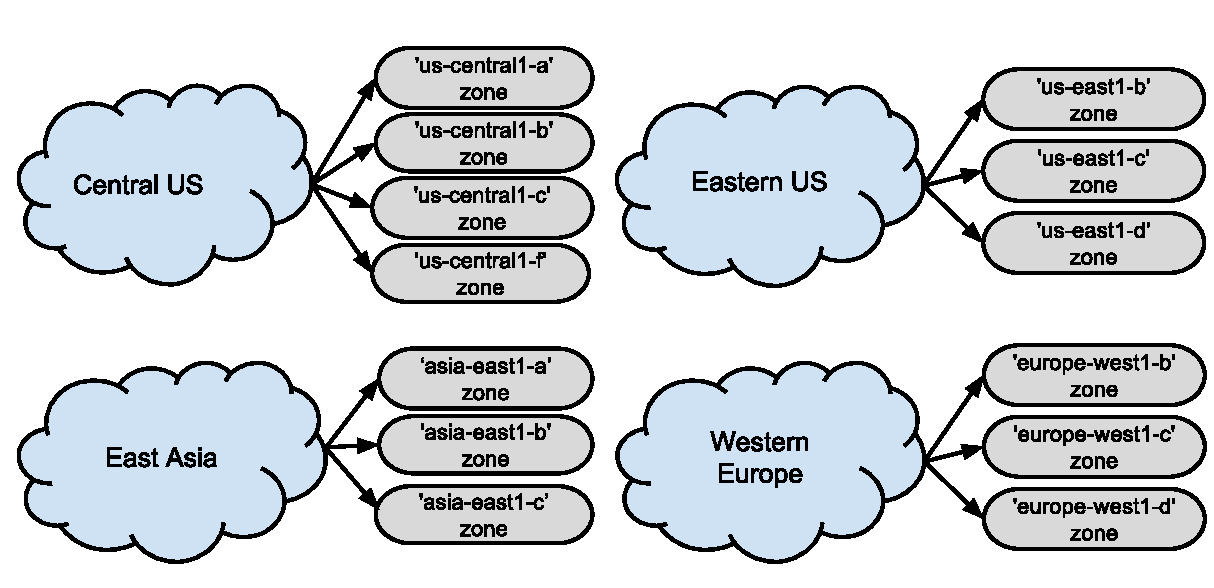
\includegraphics[width=0.7\textwidth]{./img/zones_diagram.pdf}
	%    \caption[Spatial MapReduce]{\centering Zones diagram describing zones
	%available in each region\footnotemark}
	%    \label{fig:partitioning}
	%  \end{figure}  
	%\footnotetext{Source:\url{https://cloud.google.com/compute/docs/zones}}
	
	\paragraph*{Hierarchy}
	Design of network is suited for maintaining  of custom services efficiently. The
	hierarchical model is build on separated
	levels of failure.  The room for distributing resources across multiple regions
	or zones is supported as well. Main abstract unit is \textit{location}. Each
	location consists \textit{regions}. To handle availability, locations are
	independent to each other. It make  
	network latency under 5m (on the 95th percentile) between locations. Lower
	level of hierarchy, thus subset are \textit{zones}. As well as location, 
	zones are independent to each other. Location consists of zones which should be
	classified as single point of failure. Thus, 
	to build up fault-tolerant application is necessary to deploy it over different
	zones. Furthermore, choice of region according 
	to geographic location of accessing points is essential. In addition, to
	eliminate fail of service on the level of \textit{region}, 
	Google suggests to have a backup plan for migration to another one. Fully
	qualified address of zone   for API access is \textless 
	region\textgreater-\textless zone\textgreater \ e.g. \textit{europe-west1-d}. 
	
	
	\begin{footnotesize}
		\begin{lstlisting}[style=mybash]
## view list of available zones.
$ gcloud compute zones list
NAME           REGION       STATUS NEXT_MAINTENANCE 
asia-east1-c   asia-east1   UP
..

## check available regions.
$ gcloud compute regions list
NAME         CPUS         DISKS_GB    ADDRESSES RESERVED_ADDRESSES STATUS 
asia-east1      0.00/8.00      0/2048      0/23      0/1           UP
..

## get information about desired zone e.g asia-east1.
$ gcloud compute regions describe asia-east1
creationTimestamp: '2014-05-30T18:35:16.514-07:00'
description: asia-east1
id: '1220'
kind: compute#region
name: asia-east1
quotas:
- limit: 8.0
metric: CPUS
usage: 0.0
..
		\end{lstlisting}\end{footnotesize}
	
	
	
	
	
	\subsection{Identity and Access Management}
	Cloud Identity and Access Management (Cloud IAM) provide way for handling privacy
	and permissions for \textit{Google Cloud} services. Currently, alpha  or beta
	versions are 
	supported for nine services over Google Cloud portfolio, 
	includes \textit{Google Cloud Storage}. IAM design is based on three main
	pillars, 
	such \textit{Roles}, \textit{Policy} and \textit{Resources}. The 
	identity of a user is handled by four different authentication methods such a
	Google 
	account, Service Account, Google Group and Google Apps domain.
	
	\paragraph{Resources} allows grant access to users for Cloud Platform services
	and its resources. To allow permissions for using given 
	service is declared by syntax \textless service\textgreater.\textless
	resource\textgreater.\textless verb\textgreater, for example
	\emph{pubsub.topics.publish}.
	
	\paragraph{Roles} A role represents the collection of permissions. Two kinds of
	roles 
	are available, such as Primitive roles and Curated roles. The first mentioned
	are concentric 
	roles where \textit{Owner role} can also edit and \textit{Edit role} includes 
	\textit{Read role}. This approach is applied e.g. in Cloud Storage as default.
	Second, 
	curated roles are new and allow more advanced policy management. 
	Currently (28.3.2016), \textit{Curated roles}(\ref{fig:iam}, (a) are in alpha or
	beta 
	development version and are not suggested to use for production 
	use. However, these Curated roles provide additional granular access to specific
	services 
	from Google Cloud portfolio and prevent unwanted access to 
	other resources. 
	% Please add the following required packages to your document preamble:
	% \usepackage{booktabs}
	\begin{table}[!htbp]
		\begin{scriptsize}
			\centering
			\begin{tabular}{@{}|l|l|l|@{}}
				\toprule
				Role                        & Description                                       
				
				& Permissions                                                                   
				\\ \midrule \midrule
				roles/storage.objectCreator & \begin{tabular}[c]{@{}l@{}}Allows users to create
					objects. \\ Does not give permission to delete or overwrite
					objects.\end{tabular} & storage.objects.create                                  
				\\ \midrule
				roles/storage.objectViewer  & \begin{tabular}[c]{@{}l@{}}Grants access to view
					objects and\\ their metadata, excluding ACLs.\end{tabular}                      
				& \begin{tabular}[c]{@{}l@{}}storage.objects.get\\
					storage.objects.list\end{tabular} \\ \midrule
				roles/storage.objectAdmin   & Grants full control of objects.                   
				
				& storage.objects.*                                                             
				\\ \midrule
				roles/storage.admin         & Grants full control of objects and buckets.       
				
				& \begin{tabular}[c]{@{}l@{}}storage.buckets.*\\ storage.objects.*\end{tabular} 
				\\ \bottomrule
			\end{tabular}
			\caption{Cloud Storage Roles covered by IAM}
			\label{iam}
		\end{scriptsize}
	\end{table}
	
	
	\paragraph{Policy} of Cloud IAM can grant roles to users. It is designed as a
	collection 
	of statements that specify who has what type of access. The policy is linked to
	resources 
	and control it's accessed. In Figure \ref{fig:iam}, (b) is 
	shown policy principle based on the relation between the collection of
	statements IAM and 
	Resources of Google Platform. Resources of Google Platform 
	are organized hierarchically. Figure \ref{fig:iam}, (c) demonstrated example of
	the nodes 
	in hierarchy. \textit{Organization} represent the root of 
	the hierarchy and each child has only one parent. Inheritance of hierarchy 
	handle sets and subsets of abstract classes, such as Organization, Project and
	Resources. 
	
%%% ML: zdroj ?
	\begin{figure}[!htbp]
		\centering
		%\subfloat[Roles]{ 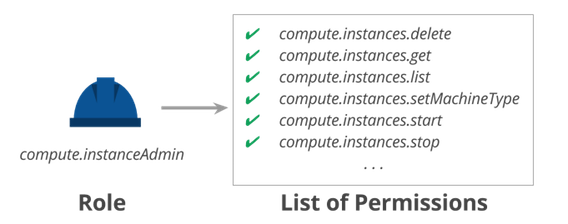
\includegraphics[width=0.4\textwidth]{./img/iamroles.png}
		%}%
		%\qquad
		%\subfloat[Cloud IAM policy management]{
		%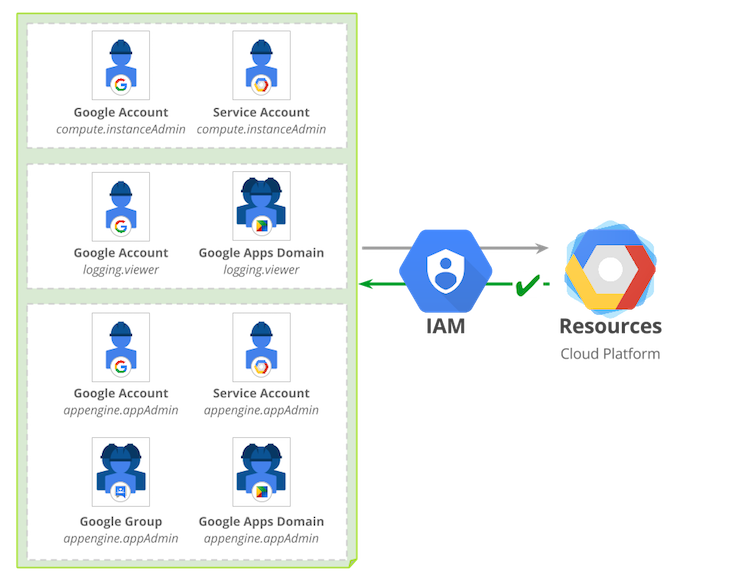
\includegraphics[width=0.5\textwidth]{./img/iampolicy.png} }%
		\subfloat[Cloud IAM Policy and Roles management]{
			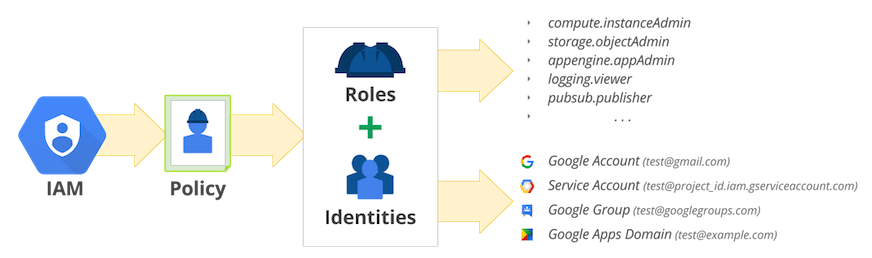
\includegraphics[width=0.8\textwidth]{./img/iam_overview.png} }%
		
		\subfloat[Policy hierarchy]{
			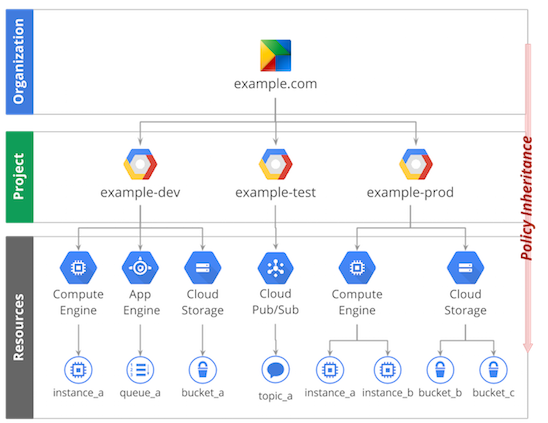
\includegraphics[width=0.7\textwidth]{./img/iampolicy-hierarchy.png} }%
		
		\caption[access]{Concepts of Cloud Identity and Access Management. Source: \url{https://cloud.google.com/iam/docs/overview} 
			\centering }
		\label{fig:iam}
	\end{figure}
	
	
	\subsection{Cloud Storage}
	\label{subsub:datastore}
	Google Cloud Storage represents service  with high level of availability and durability 
	over the world. Storage of data is highly persistent by replication data over
	Google 
	infrastructure. Service security protection is based 
	on model end-to-end, thus in-flight and at rest.  Several ways for controlling
	storage are available. Command 
	line interface \textit{gsutil} and programming API for build of 
	reliable and fast networking application. The pricing model consists of different
	tariffs 
	according to data durability, availability and performance of storage.
	
	
	\paragraph{Storage classes} are represented by three types of storages. The
	classification is derived from an characteristic of particular storage. \textit{Standard
		storage} with high availability and low 
	latency. The Standard storage suits well for frequent access such 
	as data of web services or mobile applications.
	Next class, \textit{Durable Reduced Availability} is characteristics with less
	availability than  \textit{Standard} one. 
	This class is suited for jobs, where less availability is accepted and for a
	cost-sensitive project as well. 
	Last class, \textit{Cloud Storage Nearline} fills the gap between mentioned
	classes. Attributes are of slightly lower availability and slightly higher 
	latency than Standard storage with lower cost. 
	Storage for data backup or archiving data are two explanation of use cases for
	last class.
	
	\paragraph{Buckets location} are configurable by three properties, specifically:
	global unique 
	name, storage class and geographical location where the bucket is stored.
	\begin{footnotesize}
		\begin{lstlisting}[style=mybash]
#creating two new buckets using command-line tool gsutil
$ gsutil mb -p my-project gs://mwdata gs://mwprocessed -c
durable_reduced_availability
		\end{lstlisting}
	\end{footnotesize}
	All buckets are covered under a single namespace. Thus, the name of bucket must
	be unique. 
	Google defined rules for naming buckets which are based on DNS naming
	conventions. Validator for process creation responds by error message in the wrong
	case. 
	
%%% ML: peace
%%% MK: OK
	\paragraph{Objects} holds data information placed in storage. Object has two
	components: 
	user data and metadata of quality. All \textit{objects} are immutable after
	creation. Thus, incremental changes are not available. However, an object 
	can be overwritten. Before the new version of an object is available, the old
	version is still 
	reachable for reading. Overwriting of a single object 
	can proceed up to one second. Otherwise \textit{503 Service Unavailable errors}
	is responded.
	
	\paragraph{Consistency} of data handles global Google network of data centres. 
	When success response is received, uploaded data are available from any location
	in 
	Google network. Google has designed and constructed a private network 
	for fast data transfer between their data centres around the word. Thus, data
	throughput 
	of Google backbone network is higher than the capability of the 
	internet-facing network. The latency for writing is slightly higher for
	replicated store 
	than non-replicated. Restriction of accessing metadata of object immediately
	after deletion object is good example of consistent behavior.
	It is handled by \textit{404 Not Found} status code.
	
	
	\subsubsection{Access control}
	The configuration of access control can be set using \textit{gsutil}
	command-line tool 
	or API. Cloud storage consists three different ways of buckets access
	management.
	\begin{itemize}
		\item\textbf{Access Control Lists (ACLs)} provide way to manage read or write
		access for specified Google accounts and groups.
		\item\textbf{Signed URLs (query string authentication)} provide a way to set time 
		limited read or write access to anyone who disposes of URL address. This way is
		a choice for users without Google account.   
		\item\textbf{Signed Policy Documents} allows specifying what can be uploaded to
		a bucket. 
		Size, content type and other specification can be set by policy handler. 
	\end{itemize}
	Additionally there is available access control on the Project level. For controlling 
	user's rules 
	to access bucket on the project level there is developed   \textit{Google Cloud
		Identity and Access Management} (IAM). This service is described on 
	the end of the section \ref{acl}.
	
	\paragraph{Permissions} is  divided to read and write control.
	For \textit{objects} there is available option to let user download \textit{object} 
	and modify metadata by owner.
	By default \textit{objects} are owned by original requester who 
	upload the \textit{object}. As \textit{object}, \textit{Buckets} are readable.
	In addition, list of user let them to create, overwrite and delete objects 
	in \textit{bucket}. Owner can let user to read and write permission on the
	bucket include metadata. By default, \textit{buckets} are owned by the project 
	owner group.
	
	\paragraph{Scopes}\label{par:scopes} of authentication consist of six methods for 
	specifying ACL such  Google Storage ID, Google account email address, Google 
	group email address, Google Apps domain, Special identifier for all Google 
	account holders and Special identifier for all users.
	
	\begin{footnotesize}
		\begin{lstlisting}[style=mybash]
#Identify an object that the user uploaded.
gsutil acl get gs://mwdata
		\end{lstlisting}\end{footnotesize}
	
	
	\paragraph{Access control list}\label{acl} is configurable by command line tools
	\textit{gsutil acl} or by API based on JSON or XML structures. The management of ACL is based on concentric permissions, which provide faster configuration. If user grant 
	write permission, automatically get also read permission. In case of grant of owner 
	permission, read and write is also reachable.\begin{footnotesize}
		\begin{lstlisting}[style=mybash]
#usage of a predefined ACL to an object during object upload
gsutil cp -a bucket-owner-full-control mwbck.zip gs://mwdata
		\end{lstlisting}
	\end{footnotesize}
	In addition, for quick settings of access
	restrictions such as project-private, list of predefined ACL is available:
	private, public-read, public-read-write, authenticated-read, 
	bucket-owner-read and bucket-owner-full-control.
	
	
	
	
	%\subsection{Networking}
	%https://cloud.google.com/compute/docs/networking#networks
	%https://cloud.google.com/compute/docs/vm-ip-addresses
	%%https://cloud.google.com/compute/docs/configure-instance-ip-addresses#internalstaticip
	%https://cloud.google.com/sdk/gcloud/reference/compute/firewall-rules/create
	%Rhttps://cloud.google.com/dataproc/cluster-web-interfaces
	
	
	%hive
	%https://cwiki.apache.org/confluence/display/Hive/Setting+Up+HiveServer2
	
	\subsection{Dataproc: Cluster Services}
	\label{subsub:dataproc}
	\textbf{Dataproc} is a package of tools for managing Hadoop \ref{sec:hadoop} 
	and Spark\footnote{Apache spark: \url{http://spark.apache.org/}}.
	The process of a deploying cluster is fully automatized using the default 
	configuration. Hadoop and Spark deployment are compatible with official
	releases. With default configuration, the configuration of automatic deployment is simple. 
	On the other hand in the most cases, it is 
	necessary to configure cluster manually to fulfill custom requirements. 
	Next to the standard command-line tool \textit{gcloud} there is 
	helper software \emph{bdutil}.  The tool  allows complex 
	configuration including the  
	definition of hardware configuration, combining services from wide Google cloud 
	portfolio and custom additional tasks for installation and configuration
	cluster. 
	This command-line utility are based on authentication provided by \textit{gcloud}
	interface.
	
	In the list of the main characteristic of \textit{Dataproc} solution is a 
	low cost, quick starting and integration with Google Cloud services. 
	The pricing is  \$0.01 per CPU for an hour (19.3.2016). Dataproc service can 
	include \textit{Preemptible instances} which offers pricing 
	per minutes (min 10 minutes). This choice is suitable for batch jobs and 
	fault-tolerant workloads. The time for starting cluster is up to 
	90 seconds in average. To compare e.g with Amazon cloud
	services(EMR) \cite{amazon_emr}, starting Google cluster is 3 times faster.
	
	\paragraph{Create and manage cluster} Deploying process can be handled by three
	main ways. The first one uses \textit{gcloud} command-line tool, the second by running
	\textit{bdutil} \ref{subsub:bdutil} script and the last option with using 
	\textit{Cloud Dataproc API} - \textit{cluster.create}. Google Cloud web
	interface offers framework for cluster deployment as well. On the other hand,
	the configuration and management is considerably limited. Command-line tool
	\textit{gcloud} consist of parameters: \textit{cluster} for managing and describing
	cluster, \textit{jobs} for submitting 	and managing jobs on cluster, finally parameter
	\textit{operation} for handling operation, like cancel or delete active 
	operation by \emph{operation\_id}. For more advanced cluster deployment there is	
	suited script tool \textit{bdutil} which is 
	package for custom configuration of cluster. The advantages is easy
	redeployment and	reproducibility custom	configuration of cluster. 
	
	
	
	\begin{footnotesize}
		\begin{lstlisting}[style=mybash]
#creation of cluster with default settings using command-line tool gcloud
$ gcloud dataproc clusters create <cluster-name>
		\end{lstlisting}
	\end{footnotesize}
	
	
	\paragraph{Cluster Properties} The configuration behind is not trivial but Google
	\textit{Dataproc} provides	semi-automatic deployment without big configuration investments.
	The configuration of open source software as Spark, Hadoop  and extensions as Hive	are based 
	on several XML files and plain text configuration files. For cluster deployment 
	using \textit{Dataproc}, the configuration is based on the same configuration	files. Some 
	properties are reserved by Google and cannot be overridden 
	to protect functionality of Cloud Dataproc. The crucial feature of cluster is
	immutable 	configuration after start. Thus, all configuration must be set 
	properly before daemons on cluster are started. For applying changes must be cluster
	restarted. 
	
	\paragraph{File system}
	Google Cloud Dataproc offers two different storages based on distributed
	filesystems. In chapter Hadoop \ref{subsec:hdfs} is described Hadoop Distributed File
	system (HDFS) which is default filesystem for Apache Hadoop framework and is as an optional in Google
	Services. As default filesystem for Hadoop and Spark deployment provided by Google Cloud is
	 \textit{Google Cloud storage}. 
	
%%% ML: Cloud ??? opakuje se na vice mistech...
%%% MK: jo to je blbe samozreme -OK
	Google Cloud Storage offers direct data access in available storage for the
	rest of Google 	services. In addition the interoperability provide access between Spark and
	Hadoop on Google. 	Next advantage is high data availability provided by Cloud
	Storages, with high availability and global replication without reduction of
	performance. The key feature is data access after cluster is shut down. 
	The pricing of cluster instance is based on time. Thus, to save costs, cluster
	should run only when is in use. With using HDFS as distributed filesystem, after 
	shutting down clusters VM instances, data are removed and lost as well. In contrast,
	data stored on 	Cloud Storage are available after cluster is stopped and 
	can be linked again in further cluster deployment.
	
	Interaction between Hadoop Distributed System and Dataproc cloud is limited to
	compare to default Google Storage. HDFS is scalable across VM’s, but doesn’t scale per instance as
	 well as Cloud Storage due to VM disk bandwidth limits. 
	
	\paragraph{Machine type} Google Cloud Datagram clusters are built on Google
	Compute Engine instances. \textit{Machine types} configuration defines the virtualized hardware
	 resources	available to an  virtual machine instance. Two ways how to define configuration are 
	 available: \textit{predefined instance} and \textit{custom machine types}.  
	
	\begin{footnotesize}
		\begin{lstlisting}[style=mybash]
# print list of predefined instances
$ gcloud compute machine-types list
NAME           ZONE           CPUS MEMORY_GB DEPRECATED
f1-micro       asia-east1-c   1     0.60
g1-small       asia-east1-c   1     1.70
n1-highcpu-16  asia-east1-c   16   14.40
...
		\end{lstlisting}
	\end{footnotesize}
	
	Customization of machines availability is suitable for project with workloads
	where the computing	engine requires high performance machine resources or just where predefined
	machines are not fit great to workloads. Once a custom machine template is 
	defined, the configuration is available for all connected services over Google
	Cloud portfolio.
	
	\subsubsection{bdutil: Spark and Hadoop on Google Cloud}\label{subsub:bdutil}
	As has been already mentioned, \textit{bdutil} is a command line script designed
	for	managing Hadoop instance on Google Compute Engine. It provides deployment,
	configuration	and shut-down of Hadoop instances in quickly and reproducible way, even for complex
	configuration. 	Script is based on Bash v3 or later which is available on VM of Google Compute
	Engine  and the most of Linux distributions. In addition, shell command-line tool
	\textit{gcloud dataproc}, \textit{bdutil} includes configurable scripts
	for deployment 	Spark and Hadoop. The default configuration is Hadoop 1.x with Cloud Storage as
	the storage system. Furthermore, \textit{bdutil} is designed to allow writing custom environment
	variable configuration 	files. For example: \emph{CONFIGBUCKET} - path to Google Storage, \emph{PROJECT}	
	- ID of Google Platform project or \emph{GCE\_MACHINE\_TYPE} - machine type of the Google Compute Engine.
	
	
	\section{Related Technologies Behind}
	\subsection{Geospatial Framework GRASS GIS}
	
	\textit{"\textbf{Geographic Resources Analysis Support System}, 
		commonly referred to as GRASS GIS, is a Geographic Information System (GIS) used
		for data management, image processing, graphics production, 
		spatial modelling, and visualization of many types of data. It is Free (Libre)
		Software/Open Source released under GNU General Public License 
		(GPL) $>=$ V2. GRASS GIS is an official project of the Open Source Geospatial
		Foundation."\footnote{Cited from:
			\url{https://grass.osgeo.org/documentation/general-overview/}}}
	
	\begin{figure}[!htbp]
		\centering
		
\includegraphics[width=0.2\textwidth]{./img/grasslogo.png}
		\caption[Logo GRASS]{\centering Logo of GRASS GIS.}
	\end{figure}   
%%% ML: number set of ?
	GRASS GIS vector map is a data layer which consists of feature sets in
	geographic space. These objects are represented by points, lines, areas, and volumes. Usually,
%%% ML: set of attribute and its values (zni divne) 
	each feature in the map is  connected with the set of attributes and its values.
	
	For manipulation of vector data in GRASS GIS database several drivers for interaction with different database backends are available. The main module for import and export of vectors datasets is
	v.in.ogr and v.out.ogr which is based on widely used GDAL library. In addition, new module for v.import is available. Its advantage is projection conversion on the fly during importing.
	In the current stable version of GRASS GIS is there implemented a driver for PostGIS
	support. PostGIS is an extension of object-rational PosgreSQL database which brings the support for
	geographic objects. In addition PostGIS extension consists of package of 
	location-based function for building a spatial query.  
	As PostGIS is a spatial extension for PostgreSQL, analogically ESRI Spatial
	Framework for Hadoop brings the support of spatial analysis for Hadoop and  Hive.
	
	The key feature for this project is the fact that GDAL supports reading and writing GeoJSON data
	format, which is suitable for storing and analysing data using MapReduce framework. On the other hand, there is no support for reading and writing to the unenclosed GeoJSON, and some edits of file format must be additionally done. 
	ESRI Spatial Frameworks for Hadoop allows exporting only to ESRI GeoJSON. The description of
	GeoJSON and its serialization is mandatory due to the design of MapReduce 
	for parallel computing. GeoJSON and its features are described in the second
	part of the thesis \ref{json}.
	
	
%TODO
%	\subsection{Apache Hive }
%	\textit{\footnote{Cited from: \url{https://hive.apache.org/}}"The Apache Hive ™
%		data warehouse software 
%		facilitates querying and managing large datasets residing in distributed
%		storage. Hive provides a mechanism 
%%		to project structure onto this data and query the data using an SQL-like
%		language called HiveQL. At the same
%		time, this language also allows traditional map/reduce programmers to plug in
%		their custom mappers and 
%		reducers when it is inconvenient or inefficient to express this logic in
%		HiveQL."}
	
	
	%%%%%%%%%%%%%%%%%%%%%%%%%%%%%%%%%%%%%%%%%%%%%%%%%%%%%%%%%%%%%%%%%%%%%%%%%%%%%%%%%%%%%%%%%%%%%%%%%%%%%%%%%%%%%%%%%%%%%%%%%%%
	%%%%%%%%%%%%%%%%%%%%%%%%%%%%%%%%%%%%%%%%%%%%%%%%%%%%%%%%%%%%%%%%%%%%%%%%%%%%%%%%%%%%%%%%%%%%%%%%%%%%%%%%%%%%%%%%%%%%%%%%%%%
	%%%%%%%%%%%%%%%%%%%%%%%%%%%%%%%%%%%%%%%%%%%%%%%%%%%%%%%%%%%%%%%%%%%%%%%%%%%%%%%%%%%%%%%%%%%%%%%%%%%%%%%%%%%%%%%%%%%%%%%%%%%
	%%%%%%%%%%%%%%%%%%%%%%%%%%%%%%%%%%%%%%%%%%%%%%%%%%%%%%%%%%%%%%%%%%%%%%%%%%%%%%%%%%%%%%%%%%%%%%%%%%%%%%%%%%%%%%%%%%%%%%%%%%%
	
	\newpage
	\chapter*{Experimental Framework}\stepcounter{chapter}\addcontentsline{toc}{chapter}{Practical
		framework}
	In first part of the thesis there has been introduced background of technologies which are 
	linked to further text, thus to the outputs  of this work. The text below points the 
	configuration of cluster, development of GRASS Hadoop Framework (GHF) and its usage.
	The configuration of network, cloud services and Hadoop together with case study of 
	GHF usage explain full workflow of processing spatial data using Hadoop within desktop GIS.
	
	In addition, within this work, side project focused on transformation of big data from SQL
	PostgreSQL to BigQuery is accomplished. Microwave data captured by cellular operator T-Mobile 
	stored in PostgreSQL server	consists 3 billions of rows which 
	restricts valuable interaction with database.
	
	
	\section{Setup working environment}\label{setup_w_e}
	As the main resource of data storage and computing engine for practical
	framework Google Cloud Platform has been used. Thus, all configuration of Hadoop 
	cluster, data storage, and networking is linked to cloud services. Additionally,
	development of GRASS client framework for Hadoop and consequential testing  as
	well.
	
	Google Cloud Platform offers free trial 60 days promotion for using their
	services. The offer is limited by two months or 300 \$ for whichever services
	of Google Cloud portfolio.
	
	\subsection{Set up project: gcloud}\label{setup_gcloud}
	Using Google Cloud Platform web interface has been created new project placed in
	App Engine location \textit{europe-west}. The project is characterized by Project name,
	Project ID and billing account.	On local computer has been installed Cloud SDK 
	which includes \textit{gcloud} 	and \textit{gsutil} tools for remote control Google Cloud services.
	Initialization of gcloud using command \emph{gcloud init}\footnote{To initialize
	project on remote computer 	without X Window System forwarding must be used flag 
	\emph{--console-only}.}	provide authentication process using web browser 
	and request of access to the project.
	
	Compute Engine uses a default zone and region based on information from the
	project metadata. In this case,	configuration is inherited from the Project 
	settings without an additional changes.
	
	
	\subsection{Data Management}\label{data_mgr}
	Google Data Store is used as the main data house for the project. Command
	line tool \textit{gsutil} is for  object operations over buckets of Google Storage. 
	For copying large	object is very suitable to use 	a function for slicing which allows parallel 
	downloading and uploading.
	
	For downloading object using HTTP request gsutil performs slicing of object on
	Google Storage  and preallocate space in the destination folder. 
	The final file is renamed after all slices are	processed. For downloading 
	is not required additional space on local disk. The performing of slices is configurable by parameter
	\textit{sliced\_object\_download\_threshold} which 	define a maximum number of slices. It can be 
	useful to protect the disk from overloading. For efficient uploading of large
	files is crcmod which required 	an installation  of CRC32C package. 
	
	\subsection{Networking}
	The essential network configuration is necessary  for accessing Hadoop cluster
	from outside of Google sub-network. The VM instances has internal IP and
	external IP. Both of them are dynamically attached during deployment of
	instance. Optionally it is possible to reserve external static IP and attach it to
	the VM.  For usage Hadoop for batch processing it is not necessary to configure
	user network but is necessary to configure firewall. 
	
	\begin{table}[!htbp]
		\centering
		\begin{scriptsize}
			\begin{tabular}{@{}|l|l|l|l|@{}}
				\toprule
				name                   & IP range     & allowed protocol & targets tag         
				\\ \midrule  \midrule
				default-allow-icmp     & 0.0.0.0/0    & icmp             & Apply to all targets
				\\ \midrule
				default-allow-internal & 10.128.0.0/9 & tcp:0-65535,icmp & Apply to all targets
				\\ \midrule
				default-allow-rdp      & 0.0.0.0/0    & tcp:3389         & Apply to all targets
				\\ \midrule
				default-allow-ssh      & 0.0.0.0/0    & tcp:22           & Apply to all targets
				\\ \bottomrule
			\end{tabular}
		\end{scriptsize}
%%% ML: Fix the caption
		\caption{Default configuration of firewall for accessing machines from external networks.}
		\label{my-label}
	\end{table}
	By default, incoming traffic from outside of your network is blocked. To allow
	incoming traffic a firewall rule must be set. Firewall rules regulate only incoming
	traffic to an instance. When a connection is established with an instance,
	traffic is permitted in both directions over that connection. On web of Google
	Cloud Platform there is a manager for defining of firewall rules. By default several
%%% ML: fix ref
	profiles are predefined, how was already mentioned in table \ref{firewall}.
	%https://dzone.com/articles/hadoop-rest-api-webhdfs
	
	\subsubsection{Network Configuration}\label{network_cfg}
	For  processing of data within desktop GIS to configure network is mandatory. 
	If we assume that the cluster is private and mainly for batch processing the 
	predefined network can be used. The network must be reconfigured to be accessible
	from outside of Google sub network. Configuration of two network characteristics is mandatory.
	\begin{itemize}
		\item Firewall profiles
		\item Local Hosts
	\end{itemize}
	
	\paragraph{Firewall} For using machine capacity and services on Google Cloud, 
	the installation process is described in section \textit{Setup working
		environment} \ref{setup_w_e}. The proper network configuration for connection to
	Hadoop cluster is necessary. There are several steps for basic configuration of
	Google network and local computer for batch processing. Firstly, in Google Cloud
	must be added configuration profile to firewall. Hadoop and Hive has several ports
	for their services. Java daemons have by default open ports for accessing it.
	Important ports for controlling Hadoop and Hive are 50700 for accessing NameNode, 50705 for DataNodes
	and for Hive 100000. In firewall there must be created a profile which allows access of
	these ports from outside of Google sub net\-work. To restrict access to the opens port,
	in firewall profile must be set IP address limitation. There are several option
	how to limit IP. The most common way is to define allowed IP address range. This
	configuration is suitable for single user usage. Second way is to define sub
	networks of Google Cloud. In addition is possible to allow tags of VM of Google
	Cloud. The last option is  0.0.0.0/0, thus any IP have access.
	
	\paragraph{Local Hosts}\label{hosts} For accessing HDFS from GRASS Hadoop Framework the driver must
	know all external IP addresses of master and workers of cluster. Each server has
	external IP address and local host name. The local host name is automatically generated
	during cluster deployment. In Hadoop configuration files are registered local host
	names of workers. After the client accesses HDFS daemon (port 50700) then it receives
	message with local host and port of workers instead of IP address. If the client is
	running from different machine than master, these IP addresses and local host names
	must be defined. In Linux systems the configuration of local hosts  are declared in
	file \textit{/etc/hosts}. 
	\begin{footnotesize}
		\begin{lstlisting}[style=python]
127.0.0.1       localhost
::1             localhost ip6-localhost ip6-loopback
ff02::1         ip6-allnodes
ff02::2         ip6-allrouters

10.132.0.2 cluster-2-m.c.hadoop-jakub.internal cluster-2-m  # Added by Google
		\end{lstlisting}
	\end{footnotesize}
	Master and workers, each of them has configuration similar to example of master
	machine in Google Cloud. Important is the  last line. This line must be append to local
	machine \textit{etc/hosts} file.	
	
\subsection{Hadoop Deployment}\label{hadoop_deployment}
	For deployment of Hadoop cluster there is used bdutil command line package builds from
	several bash scripts and XML configuration files of Hadoop and its extensions. 
	In the section below a essential configuration of Hadoop on Google Dataporoc 
	service is described. Mainly there is shown the important part which touches requirements for using
	ESRI Spatial Frameworks for Hadoop. The source of bdutil configuration  is in digital attachment of the work \ref{References}.
	
	Google Cloud Dataproc brings field automated deployment of Hadoop
	cluster to the cloud. To compare with manual configuration of Hadoop cluster, it allows fast and efficient
	deployment with wide options to interact with services of Google Cloud portfolio.
	
	The configuration files for \textit{'standard'} Hadoop are stored in
	\textbf{\$HADOOP\_HOME\\/conf/} and consist of primary xml files. Many of parameters values  
	are defined by default and they may be omitted in configuration files. 
	In addition, the default configuration folder includes shell file which specified environment variables of Hadoop Daemon. Default configuration folder lists:
	\begin{itemize}\label{conf_files}
		\item \textbf{hadoop-env.sh} The file specifies environment variables that
		affects JDK used by daemons. For example \textbf{\$JAVA\_HOME}, \textit{HADOOP\_HOME}.
		\item \textbf{core-site.sh}   This file informs Hadoop deamon where NameNode
		runs in the cluster. Furthermore, it  
		informs about port number used for Hadoop instance, memory limit for data
		size,  memory allocated for HDFS, and size of read and write buffers.
		\item \textbf{hdfs-site.sh}  This file contains the configuration settings for
		HDFS daemons, the Name Node, the Secondary Name Node, and the data nodes. 
		Usually the file configures block replication and permission checking on HDFS. 
		\item \textbf{mapred-site.sh}  This file contains the configuration settings for
		MapReduce daemons such the JobTracker and the TaskTracker.
	\end{itemize}
	
	In addition default configuration directory includes two text files:
	\textit{masters} and \textit{slaves}. Both includes hostname of slaves or master 
	where each line represents one host name address. 
	Master file informs about the Secondary NameNode location to Hadoop daemon. The
	\textit{masters} file at Master server contains an IP address of Secondary Name Node servers.
	The second one, \textit{slaves} on Slave server contains the IP address of the
	slave node. Notice that the \textit{slaves} file at Slave node contains only its
	own IP address and not of any other Data Nodes in the cluster.
	
	
	\paragraph{Hadoop modes} Hadoop can be deployed in several modes for different aim of usage. 
		\begin{itemize}
	    \item \textbf{Non-distributed mode} Hadoop running  as a single Java process. This mode  is suitable for MapReduce development and debugging.
	 	
		\item \textbf{Pseudo-Distributed mode}  configuration allows to run  Hadoop on
		single-node and behave
		like multi-node. It is provided by running Hadoop daemons in separate Java
		processes. To configure pseudo-distributed Hadoop must be modify
%%% ML: broken citation
		\textit{core-site.xml} and \textit{hdfs-site.xml} file \cite{hadoop_definitive}.  
		
		
		\begin{footnotesize}
			\begin{lstlisting}[style=python]
#etc/hadoop/core-site.xml:
-
<configuration>
<property>
<name>fs.defaultFS</name>
<value>hdfs://localhost:9000</value>
</property>
</configuration>


#etc/hadoop/hdfs-site.xml: 
-
<configuration>
<property>
<name>dfs.replication</name>
<value>1</value>
</property>
</configuration>
			\end{lstlisting}
		\end{footnotesize}
		
		\item \textbf{Fully distributed cluster} is an ideal approach for harnessing the
		potential of	parallel computations. The nodes are on virtualized machines with 
		assigned machine capability such a CPU, memory, and disk or deployed on physical machines. 
		The most efficient approach which is used in the production or in large clusters is an installation of Hadoop directly on the machine with Linux without virtualised environment. 
		This configuration is used for high performance spatial processing in case study of this work.
		
	\end{itemize}
	
	
	\subsubsection{Configuration - bdutil}
	In contrast to standard Hadoop deployment, a configuration in \textit{Dataproc}
	using bdutil is  extended by parameters and configuration files which handle automated deployment
	and interaction with other Google Cloud Services. 

	Tool bdutil comes with several bash scripts which set configuration
	of the cluster: type of framework- Hadoop or Spark, version of Hadoop, Hadoop
	extension (Hive, Pig) and connectors to other services of Google.
	

	\begin{table}[!htbp]
		\begin{scriptsize}
			\centering
			\begin{tabular}{@{}|l|l|@{}}
				\toprule
				Bash script                              & Description                          
				\\ \midrule  \midrule
				bdutil\_env.sh                           & \begin{tabular}[c]{@{}l@{}} The base of configuration. It is always run by bdutil.
					 \\ Must be modified \ref{bdutilenv}   \end{tabular} 	\\ \midrule
				single\_node\_env.sh                     & \begin{tabular}[c]{@{}l@{}}Deploys a
					pseudo-distributed cluster on a single VM. \\ This approach is suitable for
					testing clients etc.\end{tabular}       \\ \midrule
				hadoop2\_env.sh                          & \begin{tabular}[c]{@{}l@{}}Deploys a
					cluster with the latest stable version of  Hadoop 2.x  \\instead of the
					traditional Hadoop 1.x version.\end{tabular} \\ \midrule
				bigquery\_env.sh                         & \begin{tabular}[c]{@{}l@{}}Deploys a
					cluster with the BigQuery connector for  Hadoop installed.\\ Not compatible with
					hadoop2\_env.sh.\end{tabular}      \\ \midrule
				extensions/querytools/querytools\_env.sh & \begin{tabular}[c]{@{}l@{}}Deploys a
					cluster with Apache Pig and Apache Hive installed. \\ Not compatible with
					hadoop2\_env.sh.\end{tabular}             \\ \midrule
				extensions/spark/spark\_env.sh           & Deploys a cluster with Apache Spark
				installed.                                                                      
				\\ \bottomrule
			\end{tabular}
			\caption{Configuration of shell scripts in bdutil \cite{gc_hadoop}}
			\label{bdutil:configsh}
		\end{scriptsize}
	\end{table}
	
	
	
	\paragraph{bduitl\_env.sh}\label{bdutilenv}The main script called
	\textit{bdutil\_env.sh} consists of mandatory and free environmental variables for setting environment, hardware and configuration deployment.
	
	\begin{itemize}
		\item \textbf{Environment variables} provide the setting which refers to the id
		of the project and to 	the default bucket in GCS. The defined bucket holds SSH keys and configuration of the filesystem. In the case of usage GCS as a filesystem for Hadoop, the defined GCS is linked during cluster deployment and all files are natively accessible by standard Hadoop commands e.g copy file \textit{hadoop fs -cp  /data/* /tmp/}.
		
		\item \textbf{Hardware configuration}
		allows to specify name, shape, location and size of a cluster. Of the same importance has
		definition of machine type, with reflecting final performance of cluster and 
		pricing of service as well. In addition, the parameters 
		for a number of workers and size of the disk are also crucial.
		
		Hardware configuration allows setting of different disk sizes and type to
		master and workers. Furthermore, extra persistent disks (PDs) can be linked.
		Available virtual machines of service account can be attached to a further 
		cluster. For that case, the GCS connector must by allowed.
		
		\item \textbf{Deployment} section consists of parameters for customizing Hadoop
		installation on VMs workers and master. The configuration of GCS connector 
		allows to use it as a distributed filesystem \textit{GS} and \textit{BIGQUERRY}
		connector allows read/write access to Google BigQuery. File
		system of a cluster is set by default to GCS, the second 
		option is standard HDFS. This group consists of several paths of configuration for
		defining the destination of Hadoop installation and its related files. 
		Furthermore, it is essential to configure permission  of \textit{HDFS} data access.
		
		Parameter CORES\_PER\_MAP\_TASK and CORES\_PER\_REDUCE\_TASK must be defined as
		a decimal number which controls the number of maps and reduces slots on each node. 
		The number is computed as a ratio of the number of virtual cores on the node. 
		For example if the machine of specification \textit{ n1-standard-2} 
		is used (2 cores) and the parameter is set to 1 would have $\dfrac{2}{1} = 2$
		map/reduce slots.
	\end{itemize}
	
	\begin{table}[!htbp]
		\centering
		\begin{scriptsize}
			\begin{tabular}{@{}lll@{}}
				\toprule
				\multicolumn{1}{|l|}{File}                        & \multicolumn{1}{l|}{Name}   
				& \multicolumn{1}{l|}{Value}              \\ \midrule
				\midrule
				\multicolumn{1}{|l|}{\multirow{17}{*}{bdutil\_env.sh}} &
				\multicolumn{1}{l|}{CONFIGBUCKET}                 &
				\multicolumn{1}{l|}{mwdata\_export}     \\ \cmidrule(l){2-3} 
				\multicolumn{1}{|l|}{}                                 &
				\multicolumn{1}{l|}{PROJECT}                      &
				\multicolumn{1}{l|}{spatial-hadoop}     \\ \cmidrule(l){2-3} 
				\multicolumn{1}{|l|}{}                                 &
				\multicolumn{1}{l|}{GCE\_IMAGE}                   &
				\multicolumn{1}{l|}{debian-7-backports} \\ \cmidrule(l){2-3} 
				\multicolumn{1}{|l|}{}                                 &
				\multicolumn{1}{l|}{GCE\_MACHINE\_TYPE}           &
				\multicolumn{1}{l|}{n1-standard-2}      \\ \cmidrule(l){2-3} 
				\multicolumn{1}{|l|}{}                                 &
				\multicolumn{1}{l|}{GCE\_ZONE}                    &
				\multicolumn{1}{l|}{europe-west1-b}     \\ \cmidrule(l){2-3} 
				\multicolumn{1}{|l|}{}                                 &
				\multicolumn{1}{l|}{GCE\_NETWORK}                 & \multicolumn{1}{l|}{default}
				\\ \cmidrule(l){2-3} 
				\multicolumn{1}{|l|}{}                                 &
				\multicolumn{1}{l|}{GCE\_MASTER\_MACHINE\_TYPE}   &
				\multicolumn{1}{l|}{n1-standard-4}      \\ \cmidrule(l){2-3} 
				\multicolumn{1}{|l|}{}                                 &
				\multicolumn{1}{l|}{PREEMPTIBLE\_FRACTION}        & \multicolumn{1}{l|}{1.0}    
				\\ \cmidrule(l){2-3} 
				\multicolumn{1}{|l|}{}                                 &
				\multicolumn{1}{l|}{PREFIX}                       & \multicolumn{1}{l|}{hadoop} 
				\\ \cmidrule(l){2-3} 
				\multicolumn{1}{|l|}{}                                 &
				\multicolumn{1}{l|}{NUM\_WORKERS}                 & \multicolumn{1}{l|}{2}      
				\\ \cmidrule(l){2-3} 
				\multicolumn{1}{|l|}{}                                 &
				\multicolumn{1}{l|}{MASTER\_BOOT\_DISK\_SIZE\_GB} & \multicolumn{1}{l|}{200}    
				\\ \cmidrule(l){2-3} 
				\multicolumn{1}{|l|}{}                                 &
				\multicolumn{1}{l|}{DEFAULT\_FS}                  & \multicolumn{1}{l|}{gs}     
				\\ \cmidrule(l){2-3} 
				\multicolumn{1}{|l|}{}                                 &
				\multicolumn{1}{l|}{ENABLE\_HDFS}                 & \multicolumn{1}{l|}{false}  
				\\ \cmidrule(l){2-3} 
				\multicolumn{1}{|l|}{}                                 &
				\multicolumn{1}{l|}{ENABLE\_HDFS\_PERMISSIONS}    & \multicolumn{1}{l|}{false}  
				\\ \cmidrule(l){2-3} 
				\multicolumn{1}{|l|}{}                                 &
				\multicolumn{1}{l|}{INSTALL\_GCS\_CONNECTOR}      & \multicolumn{1}{l|}{true}   
				\\ \cmidrule(l){2-3} 
				\multicolumn{1}{|l|}{}                                 &
				\multicolumn{1}{l|}{CORES\_PER\_MAP\_TASK}        & \multicolumn{1}{l|}{1.0}    
				\\ \cmidrule(l){2-3} 
				\multicolumn{1}{|l|}{}                                 &
				\multicolumn{1}{l|}{CORES\_PER\_REDUCE\_TASK}     & \multicolumn{1}{l|}{1.0}    
				\\ \midrule
				\multicolumn{1}{|l|}{hdfs-template.xml}                &
				\multicolumn{1}{l|}{dfs.webhdfs.enabled}          & \multicolumn{1}{l|}{true}   
				\\ \midrule
				
			\end{tabular}
			\caption{Selected configuration parameters of bdutil tool}
			\label{bdutil:config.sh}
		\end{scriptsize}
	\end{table}
	\paragraph{Hadoop configuration} files  are stored in \textit{conf/hadoop1} for
	Hadoop version 1.x VM and 
	\textit{conf/hadoop2} for 2.x version both are placed within \textit{bdutil}
	base directory. In compassion to standard Hadoop configuration files, 
	these are extended by files for configuration Bigtable (Hadoop1.x), 
	BigQuery (Hadoop2.x) and GCS. Particular values of parameters are linked over
	environment variables to   the main script \textit{bdutil\_env.sh} and other
	bash files stored in directory \textit{libexec}.  The 
	example below show configuration of task tracker where the value is set by global variable 
	\textit{MAP\_SLOTS}. To call global variable must be used convention \textit{envVar name=""}.
	
	\begin{footnotesize}
		\begin{lstlisting}[style=XML]
<?xml version="1.0" encoding="UTF-8"?>
<?xml-stylesheet type="text/xsl" href="configuration.xsl"?>
<configuration>
<property>
<name>mapred.tasktracker.map.tasks.maximum</name>
<value><envVar name="MAP_SLOTS" /></value>
<description>The maximum number of map tasks that will 
be run simultaneously by a tasktracker.</description>
</property>
</configuration>
		\end{lstlisting}
	\end{footnotesize}
	
    Limitation of Hive/Pig and Hadoop initialized on the top of GS filesystem is that Pig and Hive 
    will tend to rely on multi-stage pipelines more heavily than plain Hadoop MapReduce, 
    thus they are vulnerable to eventual  consistency. There is not known straight solution.
    As workaround can be accepted transfer data from GS using explicit \textit{gs:// URIs } and likewise 
    to write the final output to GS, letting any intermediate cross-stage items get stored in 
    HDFS temporarily.
    
    As mentioned in Dataproc there are available two version of Hadoop. For two spatial
    frameworks from ESRI and HadoopGIS must be used version 1.x of Hadoop due to 
    dependency on Hive, which is in Google Dataproc and incompatible with versions Hadoop 2.x. 
    The main limitation of the versions 1.x is unsupported  YARN framework which is the 
    next generation of MapReduce framework also called MapReduce 2.0 (MRv2)\cite{yarn}.  
    The main difference between is in the architecture where JobTracker, resource management, 
    and job scheduling are split into separate daemons.
    
   
    
    \paragraph{Running cluster}\label{runcluster} is done by executing bdutil bash
    file with flags and parameters.  Flag \textit{--env\_var\_files} runs selected bash files from the 
    predefined group \ref{bdutil:configsh}. Besides predefined bash files it is possible to add a custom
    script which can be executed as well. The  order of files execution is according to the sort in the list. 
    The main script    \textit{bduitl\_env.sh} \ref{bdutilenv} is executed as the first one without presence 
    in the list. In example below there is in the list the script for downloading and compiling spatial frameworks for 
    Hadoop and their dependency. The spatial1.sh script is in digital attachment within bdutil.
	\begin{footnotesize}
		\begin{lstlisting}[style=python]
COMMAND_GROUPS+=(
'install_spatial:
spatial1.sh
'
)

COMMAND_STEPS+=(
'install_spatial'
)
		\end{lstlisting}
	\end{footnotesize}
	The script is defined by command group where is defined a path to the bash for execution.
	List of command steps is a global variable and its items appends to execution the list.
	%!!!!Staging binaries
	\begin{footnotesize}
		\begin{lstlisting}[style=python]
ROLE=$(/usr/share/google/get_metadata_value attributes/role)
if [[ "${ROLE}" == 'Master' ]]; then 
	do----
fi
		\end{lstlisting}
	\end{footnotesize}

The performance of cluster varies on particular task and user demands. 
Below there are described two cases of configuration cluster.
	
	\begin{itemize}
		\item \textbf{Case 1 - configuration for development }  This configuration of cluster
		suits well to developing  of Hadoop and Hive code or testing from client site. 
		Cluster is configured as pseudo mode.
		\begin{footnotesize}
			\begin{lstlisting}[style=python]
$ ./bdutil -P spatial-cluster --env_var_files \
extensions/querytools/querytools_env.sh,single_node_env.sh,spatial.sh deploy
			\end{lstlisting}
		\end{footnotesize}
		
		
		\item \textbf{Case 2 - configuration for computational }  To compare with configuration
		above, Case 2 is fully 	distributed deployment of cluster. For modifying  \textit{bdutil} setup configuration
		of hardware, storage etc. serves flags, which overwrite it.
		\begin{footnotesize}
\begin{lstlisting}[style=python]
$ ./bdutil -P spatial-cluster --num_workers 10 \
--machine_type n1-standard-6\
--env_var_files \
extensions/querytools/querytools_env.sh,spatial.sh deploy
			\end{lstlisting}
		\end{footnotesize}
	\end{itemize}
	
	
	
	
	\subsubsection{Configuration - gcloud dataproc}
    Second option for cluster deployment is command line tools \textit{gcloud
    	dataproc}. This tool is based on flags and parameters which define the specification
    of deployed cluster. In contrast to bdutil tools, gcloud dataproc is based on
    different system images which are releasing under versions. Currently, the latest
    version of image - 1.0 is built with Hadoop 2.x and Hive 1.2. Thus, this system image 
    supports version combination wich bdutil not. Tool bdutil has been tested with latest 
    versions of Hive and Hadoop and the GCS filesystem doesn’t work properly.  
	\begin{table}[!htbp]
		\centering
		\begin{scriptsize}
			\begin{tabular}{@{}|l|l|@{}}
				\toprule 
				file\_prefix & File            \\ \midrule \midrule
				core         & core-site.xml   \\ \midrule
				hdfs         & hdfs-site.xml   \\ \midrule
				mapred       & mapred-site.xml \\ \midrule
				yarn         & yarn-site.xml   \\ \midrule
				hive         & hive-site.xml   \\ \bottomrule
			\end{tabular}
		\end{scriptsize}
		\caption{Prefix for available configure files.}
		\label{config_table}
	\end{table}
	\paragraph{Properties} of configuration files mentioned above \ref{conf_files}
	and in table \ref{config_table} are set before deployment by parameter
	\textit{--properties} and its syntax. Below is shown example of deployment of cluster
	with two nodes. The last parameter configuring the file \textit{hive-site.xml}, 
	specifically defining the path for default source of *.jar libraries, which are
	automatically loaded to the Hive environment. \cite{gcloud_dataproc}
	\begin{footnotesize}
		\begin{lstlisting}[style=python]
gcloud dataproc clusters create cluster-2 
  --bucket mw_data --zone europe-west1-c
  --master-machine-type n1-standard-4 
  --master-boot-disk-size 500 
  --num-workers 2
  --worker-machine-type n1-standard-2 
  --worker-boot-disk-size 300 
  --image-version 1.0 
  --scopes 'https://www.googleapis.com/auth/cloud-platform' 
  --project spatial-hadoop
  --properties 'hive:'hive.aux.jars.path=file:///usr/local/spatial/<jar>'
		\end{lstlisting}
	\end{footnotesize}
    There are several notes and limitations  of the configuration, such as: 1)
    Google for protecting the functionality of Dataproc reserve same parameters and 2) the
    changes must be defined before daemons of Hadoop or its extensions start. For
    specifying more parameters it is possible to define several properties at once, by
    using a comma.

	\subsubsection{Additional Settings of Cluster}
	If the cluster is deployed using bdutil \ref{runcluster}  with parameter
	\textit{--env\_var\_files spatial.sh} this script on master server installs
	spatial packages, dependency and Java packages for serialization JSON. If the
	cluster runs by another way, the libraries must be compile manually. In attachment is described important configuration for packaging Java libraries\ref{att:java}



	\paragraph{Hive jar source} For using external libraries from Hive console it is necessary to add Java packages to Hadoop environment path or to Hive. Available are
	several ways:
	\begin{itemize}
		\item Add jar from console 
		\begin{footnotesize}
			\begin{lstlisting}[style=python]
$hive add jar ${env:HIVE_HOME}/lib/ESRI-geometry-api.jar;
			\end{lstlisting}
		\end{footnotesize}
		\item Add destination \textless path\textgreater~to Hadoop path; (works
		remotely)
		\item Add to \textit{hive-site.xml} parameter \textit{hd.hive.aux.jars.path} with
		value \textless path.jar\textgreater; (works remotely)
		\item Create in \$HIVE\_HOME directory auxlib and copy jar's there.
		\item As workaround is to export path-  export HIVE\_AUX\_JARS\_PATH= \textless
		path\textgreater; (works locally)
	\end{itemize}
	The third option is the most correct and for using GHF must be used. After
	change is applied, Hive and Hadoop daemons must be restarted. 
	%http://stackoverflow.com/questions/31802908/adding-hive-jars-permanently





    \section{GRASS Hadoop framework}
    \paragraph{Background}
    Desktop application GRASS GIS became as a powerful environment for analyzing
    spatial data, which can  reach characteristic of big data. In a box of GRASS GIS there are 
    hundreds of modules. The main motivation behind GRASS GIS framework for Hadoop is 
    a vision which allows user
    processing big vector dataset natively from desktop environment. In proprietary GIS field,
    ESRI comes with package \textit{Geoprocessing tools for Hadoop}\cite{ESRI_gtfp} 
    which has been implemented for ArcMap desktop application  as a native interface
    for interaction with  their Java library \textit{ESRI Spatial framework for Hadoop}. More
    specifically, the tools enable:
	
	\begin{itemize}
		\item exchange data between ArcGIS Geodatabase and a Hadoop system, and allows
		ArcGIS to run Hadoop workflow jobs,
		\item copy data files from ArcGIS to Hadoop, and copy files from Hadoop to
		ArcGIS, and 
		\item run an Oozie workflow in Hadoop, and to check the status of a submitted
		workflow.
	\end{itemize}
	
    Described features of ESRI approach are the source of inspiration for GRASS Hadoop framework, 
    which is developed within this work.
    
    In the first, the chapter \ref{summary_libs} of this work describes and
    summarizes features of three different frameworks for processing large-scale
    data. As the most suitable framework for this project became ESRI Framework, which
    can be deployed without extra customization, natively includes considerable
    package of spatial functions, furthermore, the documentation and examples of
    usage are the most comprehensive. The selected library is used for testing
    and for explanation of usage. Even other libraries have
    not been tested, the modular design of framework allows to partition each step
    of workflow which ensure easier future development. For example,
    user can generate GeoJSON from GRASS map and load it to HDFS using
%%% ML: doporucuji vsechny modulu pojmenovat stejnym prefixem, co tedy hd.*?
%%% ML: hd.vector.import
%%% MK:ok
    \textit{hd.hdfs.in.vector}, and after that create Hive table using
%%% ML: hd.hive.json.table+

    \textit{hd.hive.json.table} and load data. These steps are independent.
    Thus the interface for interaction between GRASS and
    Hive/Hadoop can be used as library for interaction with different Hadoop spatial library.
    Due the fact that HadoopGIS is based on Hive, the GHF supports it as well. 
    Within this work, the testing of HadoopGIS library is not provided.

	
	\begin{figure}[!htbp]
		\centering
		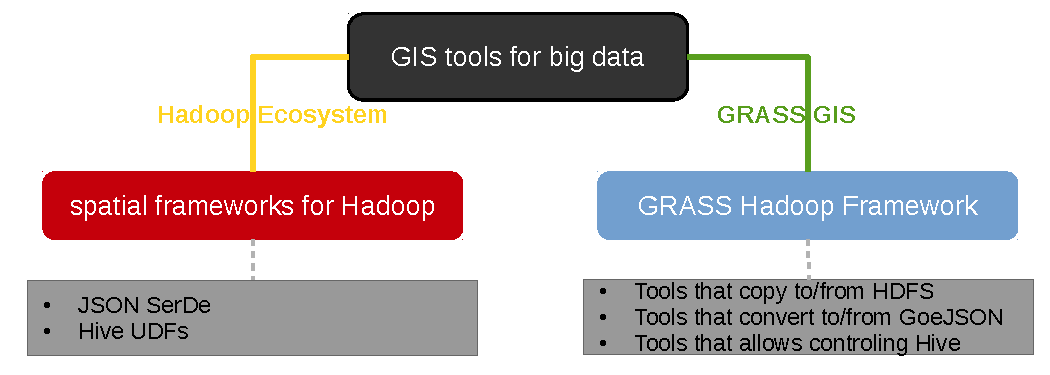
\includegraphics[width=1\textwidth]{./img/idea_schema.pdf}
		\caption[Resources]{\centering Resources for processing big data within
			desktop GIS}
	\end{figure} 
	
	
	\subsection{Functionality}
    The GRASS Hadoop Framework (GHF) is Add-ons package of modules
    for GRASS GIS. It provides interaction between GIS desktop environment and
    Hadoop/Hive. Although GHF can be used just for transferring data between filesystem
    and HDFS, the main purpose is to bring capability of Hadoop spatial
    frameworks  to the GIS desktop application. 
    
    Hadoop-based spatial libraries can be used externally from the
    command line console e.g. \textit{hiveserver2} or \textit{hadoop fs}
    command line tool. This way of usage can be more powerful for experienced users with
    administration access to the cluster and knowledge of scripting, especially in bash.
    If we assume that average user prefers friendly interface, than GHF is suitable
    choice. 
    
    The package includes several modules \ref{tbl:modules} for managing connections,
    exporting GRASS maps to customized GeoJSON (suitable for serialization), loading
    them to HDFS, creating tables in Hive, loading data into table and after
    processing, importing result back to GRASS.

%%% ML: v textu mluvis o hd.hdfs.vector.import, tady o hd.hdfs.in.vector, je potreba to sjednotit
%%% ML: k predchozi poznamce, prefix hd.hdfs. je za me taky OK i kdyz deslo
%%% ML: nazvy modulu v teto tabulce mi prijdou OK
%%% ML: sladil bycj je ale pod jednen prefix, co tedy 'hd', tj. hd.db.connect, hd.hd.hive.json.table a pod, kazdopadne by to mel byt jeden prefix!!!
%%% MK: ok
	\begin{table}[!htbp]
		\centering
		\begin{scriptsize}
			\begin{tabular}{@{}|l|l||l|l|@{}}
				\toprule
				hd.hdfs.* modules  & description                    & hd.hive.* modules  & description
				\\ \midrule \midrule
				hd.hdfs.db.connect & Management of connections      & hd.hive.json.table & Create
				table for GeoJSON  \\ \midrule
				hd.hdfs.in.fs      & Put data to HDFS from local       & hd.hive.csv.table  & Create
				table for csv data \\ \midrule
				hd.hdfs.in.vector  & Put GRASS vectors to HDFS      & hd.hive.execute    & Execute
				Hive command      \\ \midrule
				hd.hdfs.out.vector & Put vectors from HDFS to GRASS & hd.hive.select     & Execute
				Hive query        \\ \midrule
				hd.hdfs.info       & HDFS metadata                  & hd.hive.info       & Hive
				metadata             \\ \bottomrule
			\end{tabular}%
		\end{scriptsize}
		\caption{Modules of GRASS Hadoop Framework}
		\label{tbl:modules}
	\end{table}
	
	
	
    \subsubsection{Connection management} 
    The handler of connection drivers for Hadoop and Hive is covered under
    \textit{hd.hdfs.db.connect}. The module provides storing of connection profiles in
    default GRASS GIS database backend which is SQLite  by default. The usage of 
    the database manager is derived from current GRASS db.* modules.
    Thus, based on set up primary connection which is use for all involved modules.
    In contrast, database manager for HDFS allows setting
    connection id and its driver. So for each type of database (driver) can be
    stored several user connections distinctive by user defined id (\textit{conn\_ide}
    parameter) meanwhile  each driver can have only one primary connection.
	
	\begin{table}[!htbp]
		\begin{scriptsize}
			\centering
			\begin{tabular}{@{}|l|l||l|l|@{}}
				\toprule
				parameters    & description                                                     
				& flags & description                  
				\\ \midrule \midrule
				\midrule
				driver        & \begin{tabular}[c]{@{}l@{}}Type of database driver.\\ options:
					\\ hiveserver2, hdfs, webhdfs\end{tabular} & -c    & Print table of connection  
				\\ \midrule
				conn\_id      & identificator of connection                                     
				& -p    & Print active connection      
				\\ \midrule
				host          & connection host                                                 
				& -r    & Remove all connections       
				\\ \midrule
				port          & port of database                                                
				& -t    & Test connection by conn\_type
				\\ \midrule
				login         & user login                                                      
				& -a    &
				\begin{tabular}[c]{@{}l@{}}Set active connection\\  by conn\_id and
					driver\end{tabular} \\ \midrule
				passwd        & password to database                                            
				& --h   & Print usage summary          
				\\ \midrule
				schema        & set active schema in db.                                        
				& --v   & Verbose module output        
				\\ \midrule
				authmechanism & support PLAIN mechanism                                         
				& --q   & Quiet module output          
				\\ \midrule
				connectionuri & connection uri of database                                      
				& --ui  & Force launching GUI dialog   
				\\ \midrule
				rmi           & Remove connection by id                                         
				&       &                              
				\\ \bottomrule
			\end{tabular}
			\caption{Flags and parameters of \textit{hd.db.connection} module.}
			\label{tbl:connections}
		\end{scriptsize}
	\end{table}
    
    \paragraph{Defining connection} Parameter \textit{driver} and \textit{conn\_id}
    are mandatory for each connection profile. Parameter \textit{driver} defines the
    protocol for communication with database and  \textit{conn\_id} is a free
    unique string of connection profile. Other parameters as \textit{host},
    \textit{port}, \textit{login}, \textit{passwd}, \textit{schema},
    \textit{authmechanism} depends on a configuration of database server. After a new
    connection is added, the module automatically set the new one as active. 
    
    \paragraph{Connections management} Module offers several flags for handling
    management of connections. In table \ref{tbl:connections} there are described flags and
    theirs functions. In case of controlling several Hadoop clusters it is suitable 
    to define its connection profiles and switching between by flag -a with parameter
    \textit{conn\_id} and \textit{driver}.
    

    \subsubsection{GRASS HDFS interface}
    The modules starts with prefixes \textit{hd.hdfs.*}(exclude \textit{hd.db.connection})
    provide tools for transferring data between GRASS maps or filesystem and Hadoop
    distributed filesystem. In addition the module \textit{hd.hdfs.info} provide basic
    metadata of files stored in HDFS.
    
    \paragraph{HDFS metadata} Module \textit{hd.hdfs.info} currently supports several
    the basic operation for check if path exists, recursive listing of directories and
    creating HDFS directory.
    
    %TODO run cluster and show output
    
    \paragraph{GRASS Map to HDFS} Vector maps in native GRASS format are not
    suitable for serialization which is needed to exploit the potential of
    spatial frameworks for Hadoop. The effective way and in the most cases the only
    possible is to store spatial data in JSON, especially GeoJSON. This format suits well  
    for serialization and library for reading is available in 
    catalog of Hive. 
    
    Module \textit{hd.hdfs.in.vector} supports transformation of GRASS map to1
    GeoJSON format and transfer to HDFS. Behind the module there are two main steps. Firstly, the map is
    converted to GeoJSON using \textit{v.out.ogr} and edited to format which is
    suitable for parsing by widely used SerDe functions for Hive. After that,
    custom GeoJSON format is uploaded to the  destination on HDFS. By default, the
    HDFS path is set to \textit{hdfs://grass\_data\_hdfs/\textless LOCATION\_NAME
    	\textgreater/\textless MAPSET \textgreater /vector}.
    
    In addition, hd.hdfs.* package also includes module \textit{hd.hdfs.in.fs} which allows
    transfer of external files to HDFS. Usage of this module becomes important for
    uploading CSV or GeoJSON files outside of GRASS. For uploading external GoeJSON files to HDFS it is
%%% ML: neplatna reference
%%% MK: ok
    necessary to modify its standardized format. The serialization  for
    JSON has several formatting requirements. %TODO add ref
	
	\begin{itemize}
		\item Each vector feature must be on separated/new line.
		\item Brackets must be at the same line.
		\begin{footnotesize}
			\begin{lstlisting}[style=python]
// this will work
{ "key" : 10 }

// this will not work
{
"key" : 10 
}
			\end{lstlisting}
		\end{footnotesize}
		
		%{footnotesize}
		\item Header of GeoJSON must be erased. For GeoJSON exported by
		\textit{v.out.ogr} it means to remove first 5 lines and last 3.
		\begin{footnotesize}
			\begin{lstlisting}[style=python]
//GeoJSON format. Not possible to serialize
{
"type": "FeatureCollection",
"crs": { "type": "name", "properties": { "name": "urn:ogc:def...

"features": [
{ "type": "Feature", "properties": { "cat": 546 }, "geometry":...
{ "type": "Feature", "properties": { "cat": 539 }, "geometry":...
]
}

// possible to serialize
{ "type": "Feature", "properties": { "cat": 546 }, "geometry":...
{ "type": "Feature", "properties": { "cat": 539 }, "geometry":...
			\end{lstlisting}
		\end{footnotesize}
	\end{itemize}
	
	
	
    \paragraph{HDFS GeoJSON to GRASS map}
    Module \textit{hd.hdfs.out.vector} handles results to get back from HDFS.
    The module download de serializes GeoJSON file from HDFS and in the second step
    modifies file to standard GeoJSON format. The second step is important to make
    file consistent according to GeoJSON standard. In that time, format is readable
    by \textit{v.in.ogr} which is based on GDAL library and can be transformed
    to the native vector map format.
    \begin{figure}[!htbp]
    	\centering
    	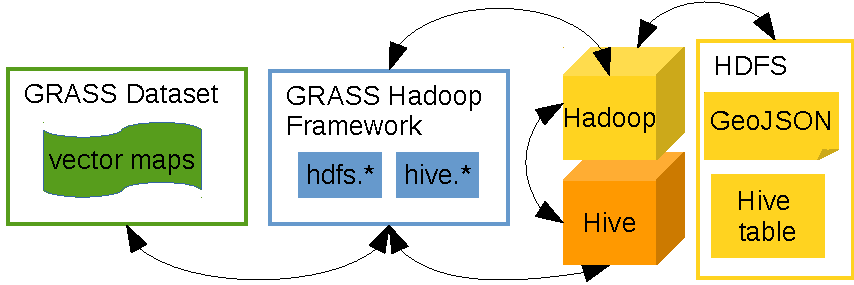
\includegraphics[width=1\textwidth]{./img/ghf_overview.pdf}
    	\caption[Components interaction]{\centering Components interaction}
    \end{figure} 
    \subsubsection{GRASS Hive interface}
    Two spatial frameworks, from ESRI and HadoopGIS use Hive as a top layer for
    usage MapReduce-based library in more expressive way. The GRASS Hadoop Framework
    consist several modules which start with prefix hd.hive.* analogically to mentioned
    hd.hdfs.* modules. Module for connection to Hive is covered by module
    \textit{hd.hdfs.db.connect} which is an exception in naming nomenclature. The
    "hive"~modules provide functions for creating tables and loading data into.
    Furthermore, module for select queries and execute commands is available. Main
    two modules \textit{hd.hive.csv.table} and \textit{hd.hive.json.table} support 
    user-friendly creation of tables and loading data into. The process of creation table
    and loading data can be split. The hd.hive.*.table modules support creation table
    without loading data. This step can be provided by module \textit{hd.hive.table.load} or
    simply by Hive command using \textit{hd.hive.execute}.
    

	
    \paragraph{Creation of table} Spatial Framework from ESRI supports reading  from
    several file format.  The Framework allows creating geometric data type from 
    WKB, JSON and GeoJSON. Table can be created from \textit{hiveserver2} command
    line or with using developed module  \textit{hd.hive.json.table} within GHF. 
    Defining feature of table is provided using parameters and flags of module. It helps
    to user make table with GeoJSON table without advanced knowledge of Hive
    syntax. In table \ref{hd.hive.json} there are described main features of each parameter.
    The examples of usage are shown in the next section \ref{sec:usage_spatial}.
    The second, slightly modified module, supports creation of table suited for loading
    CSV data. In hd.hive.* package there is also module for loading data to table. This
    module is optional because is built-in for hd.hdfs.*.table modules. 

	
	
	\begin{table}[!htbp]
		\begin{footnotesize}
			\centering
			\begin{tabular}{@{}|l|l||l|l|@{}}
				\toprule
				parameter  & description                                                        
				& flag & description     
				\\ \midrule  \midrule
				driver     & \begin{tabular}[c]{@{}l@{}}Type of database driver\\ options:\\
					hive\_cli,hiveserver2,\end{tabular}                        & -e   & create
				external table        \\ \midrule
				table      & name of table                                                      
				& -o   & overwrite data
				in table      \\ \midrule
				attributes & \begin{tabular}[c]{@{}l@{}}python dictionary\\
					\{attribute:datatype\}\end{tabular}                                         & -d
				& firstly drop table if exists \\ \midrule
				struct     & structure of json                                                  
				&      &                 
				\\ \midrule
				stored     & output format                                                      
				&      &                 
				\\ \midrule
				serde      & \begin{tabular}[c]{@{}l@{}}java class for serialization of json\\
					default: org.openx.data.jsonserde.JsonSerDe\end{tabular} &      &               
				\\ \midrule
				outformat  & java class for handling output format                              
				&      &                 
				\\ \midrule
				jsonpath   & hdfs path specifying input data                                    
				&      &                 
				\\ \bottomrule
			\end{tabular}
			\caption{Description of \textit{hd.hive.json.table} parameters and flags}
			\label{hd.hive.json}
		\end{footnotesize}
	\end{table}
	
    \paragraph{Select and execute} In the package there are two additional modules for
    advanced commands. The module \textit{hd.hive.select} is intended for building custom query
    and produce the result according to standard  output or to the file. The second one, module for
    execution can be used for any command. In contrast, that works properly only with
    non-optimised query type, when creating table, loading data, dropping databases
    etc.  Consequently, it queries without complex output.
	
		
	\subsection{Implementation}
	Package GRASS Hadoop Framework has been developed in Python language. The
	background of the choice of Python language is clear. GRASS GIS natively
	supports Python and GRASS libraries are fully covered by API. As GRASS GIS modular design, the
	user interface of package GRASS Hadoop Framework is modular as well. The user
	interface of GHF is provided by command line modules. 
	The design of framework is based on three layers: (1) the core library, (2) the middle
	interface and  (3)the top level interface. The core library of presented project represent
	wrappers for HDFS, Hive drivers and its management of connection. The middle
	interface consist of factories for the top level interface, thus modules accessible
	from GRASS GIS user interface.
	
	\begin{figure}[!htbp]
		\centering
		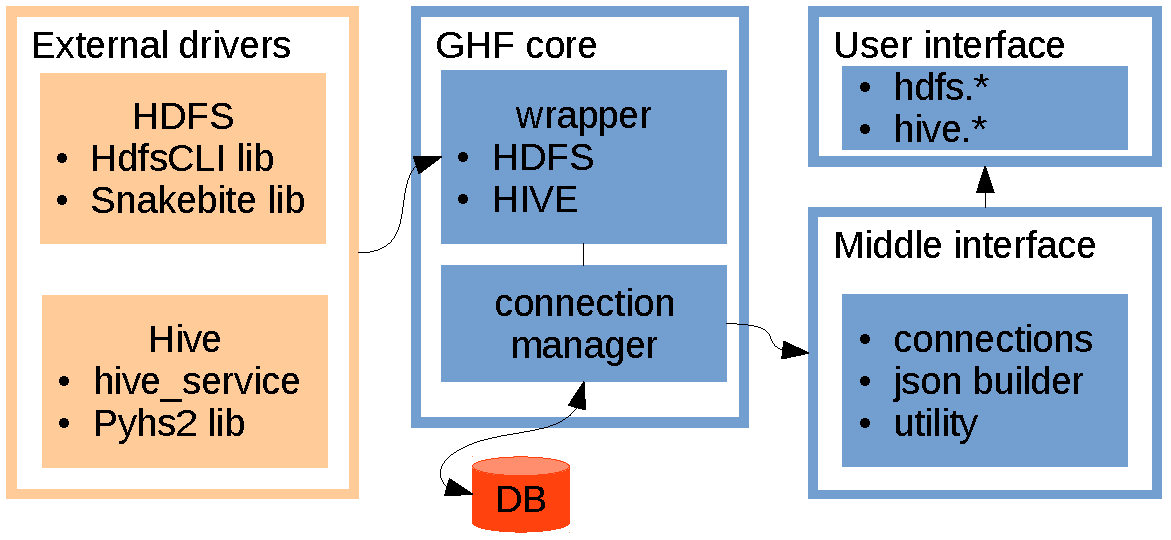
\includegraphics[width=1\textwidth]{./img/implementation.pdf}
		\caption[Architecture of GHF]{\centering Architecture of GRASS Hadoop
			Framework}
	\end{figure} 
	
	
	\subsubsection{External libraries (drivers)}
	In this section introduction to the external libraries for interaction with HDFS
	and Hive, which are used in GHF, is provided. 
	
	\paragraph{HDFS libraries}
	For communication with HDFS two libraries are used. The first one, wrapper of
	\textit{HdfsCLI} command line shell which is primary developed to make
	interaction with HDFS more intuitive than standard \textit{hadoop fs} command
%%% ML: ANSI formatting?
%%% MK: ok
	line shell. It has features as completion and command history.
%%% ML: tato veta zni divne (For this tool...)
%%% MK: ok
	The commandline  tools is wrapped by python library which is used within GHF. The controlling of
	remote HDFS is based on WebHDFS REST API and HttpFS supporting both secure and
	insecure clusters.
	
	The second library which has been developed within Spotify project is called
%%% ML: zni divne: This library is as well as first 
%%% MK: ok
	Snakebite. This library is shared under Apache licence, Version
	2.0. The library is written as pure HDFS client to eliminate expensive calling
	\textit{hadoop} from Python. The HDFS client instead of calling hadoop uses
	Protocol Buffers, which  are a language-neutral, platform-neutral extensible
	mechanism for serializing structured data.\cite{protobuf}. Snakebite relies on
	protobuf messages and implements the Hadoop RPC protocol description for talking
	to the NameNode.\cite{snakebite}
	
	\paragraph{Hive libraries}
	Similarly to HDFS interaction, Hive uses also two libraries. The first
	called \textit{pyhs2} is for interaction with \textit{hiveserver2}. It includes all
	required packages such as SASL and Thrift wrappers. The second used library is
	\textit{hive-thrift-py}. From this Thrift based library there is used only module for
	accessing meta-store of Hive.
	
	\subsubsection{GHF core}
	The core provides API for the middle interface and  consists of functions for
	interaction with HDFS and Hive database. More specifically, it allows to put/get
	data to/from HDFS and interacts with HDFS using essential filesystem commands.
	The part focused on Hive interaction allows to create specific table for
	loading CSV and JSON files, fetch metadata from meta store of Hive and execute
	non-optimized queries or fetch result of select query. In the core library there is
	used part of the code from \textit{Airflow} project, which is currently in
	incubator of Apache \cite{airflow_diff}. 
	The core library consists mainly from wrappers on
	the mentioned external libraries. The classes of core library can be parted to
	the  wrappers (hooks) and to the connection manager. 
	
	\begin{figure}[!htbp]
		\centering
		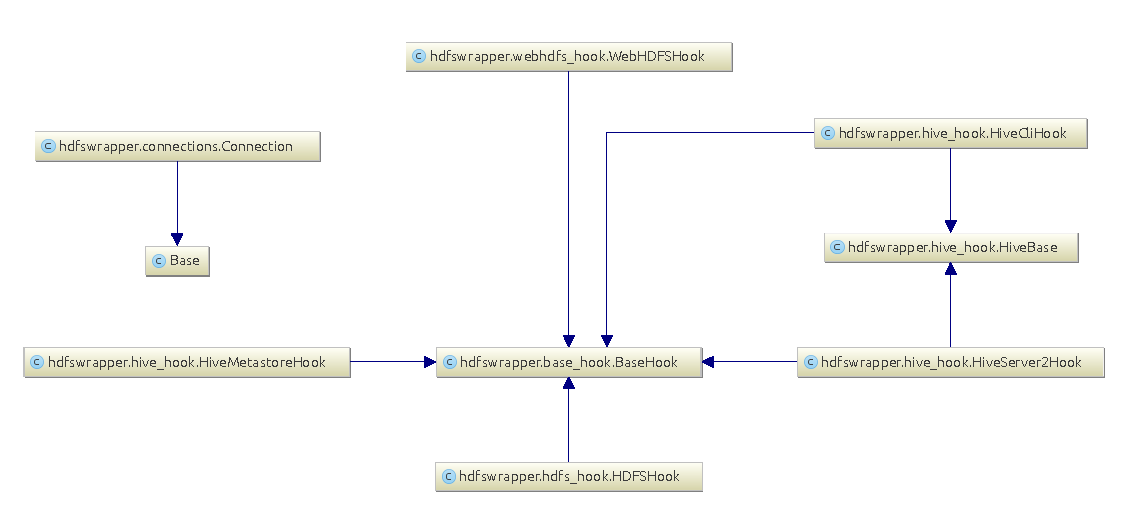
\includegraphics[width=1\textwidth]{./img/diag1_small.pdf}
		\caption[Core diagram]{\centering Design of the core library }
	\end{figure} 
	
	\paragraph{Connection} management on the  lower level is handled by  class
	\textit{Connection}. The class is a place holder to store information about
	different database instances. The class inherits the base class for declarative
	class definitions of SQLAlchemy library. 
	It allows to use ORM SQL in expressive/programmatically way.  
	\begin{footnotesize}
		\begin{lstlisting}[style=python]
from sqlalchemy.ext.declarative import declarative_base
Base = declarative_base()

class Connection(Base):
__tablename__ = "connection"
id = Column(Integer(), primary_key=True)
conn_id = Column(String(ID_LEN),unique=True)
conn_type = Column(String(500))
		\end{lstlisting}
	\end{footnotesize}
	The class ensures integrity of initialization of \textit{connection} table in
	database and the main access point for getting hooks of each connection type,
	such a hdfs hook, hive hook etc. 
	\begin{footnotesize}
		\begin{lstlisting}[style=python]
def get_hook(self):
"""End point for accessing hooks"""
if self.conn_type == 'hiveserver2':
return hive_hook.HiveServer2Hook(HiveServer2Hook=self.conn_id)
elif self.conn_type == 'webhdfs':
return webhdfs_hook.WebHDFSHook(webhdfs_conn_id=self.conn_id)
		\end{lstlisting}
	\end{footnotesize}
	After initialization of instance for the \textit{Connection} class method
	\textit{get\_hook} returns connection hook according class variable
	\textit{conn\_id}, which is an unique identifier for each group of connection
	type, such as \textit{hiveserver2}, \textit{webhdfs} etc.
	
	\paragraph{Connection hooks}
	Python modules called \textit{*\_hook.py} consist of classes which inherits from
	the class \textit{BaseHook} stored in module \textit{base\_hook.py}.
	\textit{BaseHook} is an abstract class for hooks and return of object that can
	handle the connection and interaction to specific instances of these systems
	and expose consistent methods to interact with them.
	
	Modules \textit{*\_hook.py} and their hook classes provide wrappers on the
	external libraries. Module \textit{hdfs\_hook.py} and \textit{webhdfs\_hook.py}
	provide essential functions as put data to HDFS, get data from HDFS, make
	directory, check if path exists etc. 
	The module \textit{ hive\_hook.py} consist three classes. The class
	\textit{HiveServer2Hook} allows to interact with \textit{hiveserver2} CLI. The
	second class is a simple wrapper around the hive CLI. It also supports beeline
	Hive CLI, which is lighter due to independence on JDBC. Third class of this
	module -  \textit{HiveMetastoreHook} provide access to meta store of Hive. 
	
	\subsubsection{Middle Interface and GHF Modules}
%%% ML: veta "The Main ... " zni divne
%%% MK: ok
	The middle interface consists of two Python modules. The first one, called
	\textit{hdfs\_grass\_lib.py}, which includes classes for Connection management
	and GeoJSON conversion.  The second module called \textit{hdfs\_grass\_util.py}
%%% ML: their ?
%%% MK: ok :)

	is its helper. This interface allows to developed command lines
	modules. These modules mainly call API according to parsed parameters and flags.  
	
	Class \textit{JSONBuilder} and class \textit{GrassMapBuilder} are API for
	conversion between GRASS native vector map and GeoJSON.  \textit{JSONBuilder}
	convert GRASS map to GeoJSON and modify the text file to the form, which is
	suitable for serialization. In contrast, the class \textit{GrassMapBuilder}
	convert exported map from HDFS to the format, witch is readable by
	\textit{v.in.ogr} module. It means transformation of the result from processed analysis back
	to the GRASS native format.
	
	\paragraph{GHF modules}
	Already introduced modules hd.hdfs.* and hd.hive.* as a user interface and endpoint
	for accessing GHF from GRASS GIS user environment are developed accordingly to
	GRASS "standard", where the GRASS parser read input flags and parameters. GRASS
	parser is a function, which parse the header of Python module.  Rules of syntax
	allow to comfortably interact with GRASS environment variables. Moreover, GRASS
	parser works with any programming language. In addition, \textit{g.parser} can display
	an auto-generated GUI interface, help page template, and command line option
	checking. 
	Below is a part of parsed lines from the module \textit{hd.hive.json.table}.
	\begin{footnotesize}
		\begin{lstlisting}[style=python]
# %option
# % key: driver
# % type: string
# % required: yes
# % answer: hiveserver2
# % description: Type of database driver
# % options: hiveserver2
# %end
# %flag
# % key: d
# % description: Firstly drop table if exists
# % guisection: table
# %end
		\end{lstlisting}
	\end{footnotesize}
	The first option is a parameter for defining values of driver. This parameter is
	mandatory and currently has only one possible value. The second is a flag for
	dropping table, before creation the new on. This flag is in the
	\textit{guisection} table, which is after generating GUI form the notebook
	page. Below there is example of initialization and usage of \textit{g.parser}.
	\begin{footnotesize}
		\begin{lstlisting}[style=python]
import grass.script as grass

def main():
grass.message(options['driver'])
grass.message(flags['-d'])

if __name__ == "__main__":
options, flags = grass.parser()
main()
		\end{lstlisting}
	\end{footnotesize}
	See below the executed script from GRASS environment.
	\begin{footnotesize}
		\begin{lstlisting}[style=python]
$ hd.hive.json.table hiveserver2 -d
out> 
hiveserver2
true
		\end{lstlisting}
	\end{footnotesize}
	
%%% ML: co pridat screenshot vygenerovaneho GUI na ukazku??

%%% ML: predpokladam, ze nahrajeme behem tohoto tydne (utery, streda)
	\paragraph{GRASS Add-ons package} The GHF has been published to GRASS Add-ons
	repository. GRASS module \textit{g.extension} allows to fetch and deploy packages
	from Add-ons to the GRASS environment. Each package in Add-ons must include HTML
	manual site and Makefile for proper deploy. 
	
	
	
%%% ML: tohle patri spis do prilohy (minimalne instalace) nez do textu!!!
%%% MK predelano
	\section{Usage: Process Workflow}\label{sec:usage_spatial}
	This section shows  developed GRASS Hadoop Framework in use. Two main groups of particular tasks covers the full spatial processing workflow.
	\begin{enumerate}
	\item Setup working environment: cluster and client computer\ref{prereq}
	\item Spatial analysis: processing spatial data using Hadoop within GRASS GIS\ref{spatial_anal_usage}
	\end{enumerate}
	The second group is partly focused on description of
	Hive usage, such as serialization/deserialization of GeoJSON
	and its limitation with different libraries.
	
	\subsection{Prerequisites}\label{prereq}
	To fulfil prerequisites for usage of computational power of Google Cloud for spatial analysis several steps must be done.
	

	\begin{enumerate}
	\item Set up project\ref{setup_gcloud} in Google Cloud and configure storage\ref{data_mgr};
	\item Configure networking\ref{network_cfg};
	\item Configure and deploy Hadoop cluster with Hive\ref{hadoop_deployment};
	\item Install all prerequisites on cluster\ref{att:java};
	\item Install all prerequisites on client computer\ref{grass_install};
	\item Configure hosts on local computer\ref{hosts}
	\end{enumerate}


	After finalising of each particular step the status should be: Hadoop cluster is configured and running on Google Cloud, all dependencies on cluster are installed, Goggle network allows to connect on Hadoop from local computer and GRASS GIS and GRASS Hadoop Framework is installed. If all works well the processing of data can start. 
		\begin{figure}[!htbp]
			\centering
			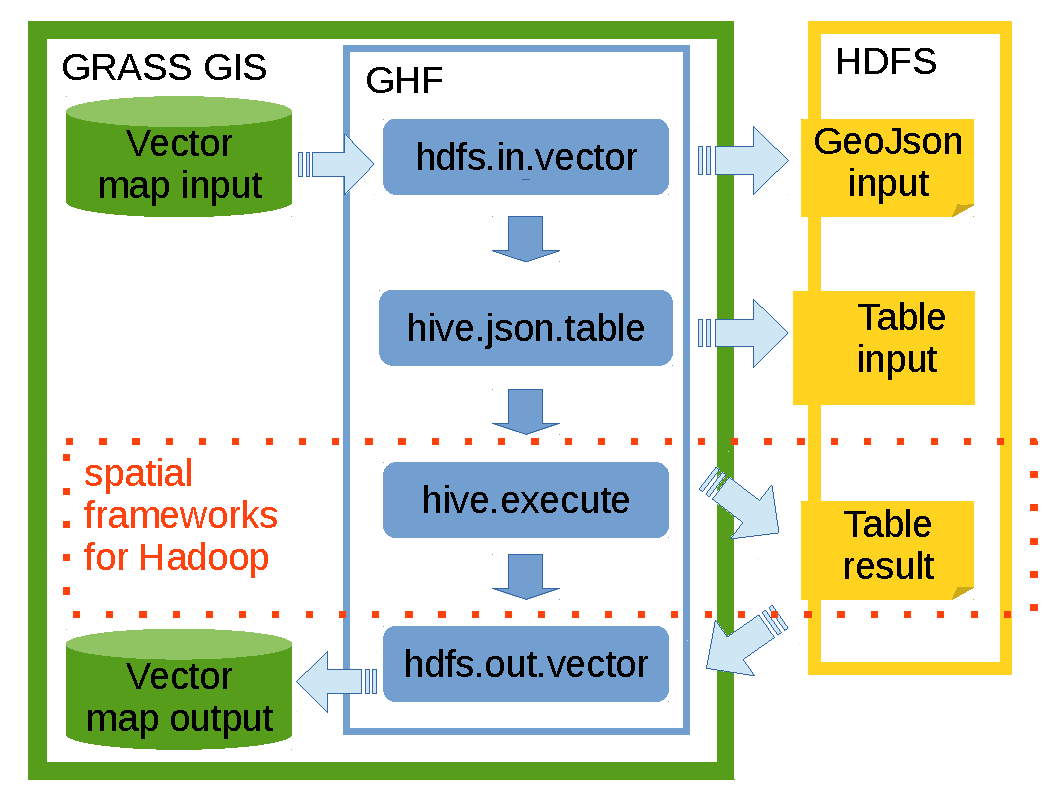
\includegraphics[width=0.8\textwidth]{./img/modules_schema.pdf}
			\caption[GHF workflow]{\centering Process workflow of GRASS Hadoop Framework 
			}
			\label{wokrflow}
		\end{figure} 
		
	
	\subsection{Test case: Spatial Binning}\label{spatial_anal_usage}
	The section Spatial Analysis shows GRASS Hadoop framework in use, especially 
	the interaction with ESRI Spatial library for Hadoop. 
	At the first part introduction of work aims on service management that allows 
	the second of part of workflow to start and proceed. This part includes preparation of data
	and querying Hive database. In addition it includes usage of functions from ESRI
	Spatial Framework for Hadoop.
	
	The main goal suppose to create time series dataset, which show partial contribution to Open
	Street Map for each year. The motivation behind this task is to recognize which areas of
	Europe are more touched by contributions and which year open street map
	project registered boom. Europe data extraction of Planet dataset from
	Open Street Map repository covers area of Europe\footnote{source of dataset
	\url{http://osm.personalwerk.de/full-history-extracts/latest/continents/}} 
	and includes all history of changes  within the project. The size of compressed
	dataset(pbf compression) of 
	Europe is 23 Gb and consists approximately 1,3 billions of points.
	The goal of this case study is to create density map of partial contributions in time
	resolution of one year. For this kind of analyses it is suitable to use spatial
	binning. Data binning is a data pre-processing technique used to reduce the
	effects of minor observation errors\ref{bining}. The original data values which
	fall in a given small interval, a bin, are replaced by a value representative of
	that interval or just add to. It is a form of aggregation used for
	generalization and for creation of density maps.
	
	
\subsubsection{Preparation of data}
\paragraph{Data to HDFS}
	 The tool Osmconvert\footnote{Osmcomverter web
	page\url{http://wiki.openstreetmap.org/wiki/Osmconvert}} allows to transform
	binary file to csv,  where each 	\textit{@} after \textit{--csv} parameter
	defines column of data.
	\begin{footnotesize}
		\begin{lstlisting}[style=python]
$ osmconvert italy.osh.pbf  -o=europe.csv --csv-separator=, \
                            --csv="@id  @lon  @lat  @timestamp"
		\end{lstlisting}
	\end{footnotesize}
	 After conversion, the size of file is 116Gb. Without writing special Hive
	UDF(User Defined Function) the timestamps of exported file must edited to proper
	\textit{datetime} format. Using \textit{sed} command line tool it is easy even
	for big data.
	\begin{footnotesize}
		\begin{lstlisting}[style=python]
$ sed "s/T/ /g"
		\end{lstlisting}
	\end{footnotesize}
	 	Available are two ways how to put file to distributed filesystem . If GS
	filesystem is used and cluster is deployed using bdutil, than the best way to
	load data is to bucket which cluster is used. 
	In more common way, using Hadoop and
	its \textit{hadoop fs} tool can be used to put data to HDFS.
\begin{enumerate}
\item HDFS  - loading data to the default distributed filesystem of Hadoop.
	\begin{footnotesize}
		\begin{lstlisting}[style=python]
$ hadoop fs -put europe_latest_fix.csv /data/
		\end{lstlisting}
	\end{footnotesize}
\item Google Storage - loading data to bucket of GS, below is shown used slicing of
file which speed up uploading process.
	\begin{footnotesize}
		\begin{lstlisting}[style=python]
$ gsutil -m -o GSUtil:parallel_composite_upload_threshold=150M cp /
		 europe_latest_fix.csv gs://data/
		\end{lstlisting}
	\end{footnotesize}
\end{enumerate}
	This ensures that file is distributed over cluster to blocks. In addition
	according  configured number of replication, data is replicated over DataNodes.
	By default replication is set to 2.
	Above is shown approach where data are downloaded directly to the server.
	However, in some cases user cannot control the cluster directly, only over
	WebHDFS access. For this case it is suitable to use module \textit{hd.hdfs.in.fs}
	which support that.
	\begin{footnotesize}
		\begin{lstlisting}[style=python]
# copy local file to HDFS on server
$ hd.hdfs.in.fs  driver=webhdfs hdfs=/data local=europe_latest_fix.csv
		\end{lstlisting}
	\end{footnotesize}
	The HDFS folders and files can be check by module \textit{hd.hdfs.info}
	\begin{footnotesize}
		\begin{lstlisting}[style=python]
# print path recursively
$ hd.hdfs.info  driver=webhdfs path=/data -r
		\end{lstlisting}
	\end{footnotesize}
	
	Below continue analyses focused on visualization of Europe contribution to Open Street Map. 
	In attachment\ref{hdfs2grass} is shown several steps which make further binning only for Czech
	Republic area. Usage of \textit{ST\_Contain} is shown. 
	

\subsubsection{Loading data to Hive}
	Below, in next section is described usage of Hive data warehouse. Mainly
	creating tables and inserting data into. In examples are shown HQL query
	together with examples of GHF equivalents.
	
	Similarly to process of establishing connection to HDFS,
	 the connection must be set connection for Hive.
\begin{footnotesize}
	\begin{lstlisting}[style=python]
#connection using wrapper around hiveserver2
$ hd.db.connect driver=hiveserver2 \
		conn_id=hiveserver2_id \
		host=cluster-4-m.c.hadoop-jakub.internal \
		port=10000 \
		login=matt \
		schema=default 
	 		
...
      Test connection (show databases;) 
              [['default']]
		\end{lstlisting}
	\end{footnotesize}
	By executing query \textit{'show databases;'} module tests if the connection
	passed. If the test fails, it returns connection error message.
	
	
		Module \textit{df.hive.json.table} allows to load exported GeoJSON data to
	table. ESRI implements Java libraries for serialization ESRI GeoJSON which is
	supported by GDAL only for reading. Thus for serialization of GeoJSON another library must be
	used. There are several libraries available. The most widely used is
	from onix. In attachment \ref{serde} several notes is added about serialization
	JSON.

\paragraph{Table europe}
		The 116 Gb csv file which consists all points over the history of Open Street
	Map on the area covered by Europe is separated by comma and without header. For this csv
	format without extra features it is possible to use built-in function for
	serialization which is initialized by \textit{ROW FORMAT DELIMITED FIELDS
	TERMINATED BY ',';} expression.
		
	Some benchmarks discussed on web site of
	\textit{HortonWorks}\footnote{\url{http://tinyurl.com/hvvr5nt}} point that the fastest serialization of csv is reached using native approach. Benchmark shows
	that library \textit{org.apache.hadoop.hive.serde2.OpenCSVSerde} is 3x slower
	than native csv reader. On the other hand, OpenCSVSerde allows to pares CSV with
	strange delimiters, such blanks.
		
		
	Table \textit{euro}pe according to CSV of Open Street Map data has columns: \textit{id, lat, lon
and time.}
\begin{footnotesize}
	\begin{lstlisting}[style=python]
#cretion of table for Europe dataset withinhive command-line
CREATE EXTERNAL TABLE europe(id BIGINT,
                            lat DOUBLE,lon DOUBLE,
                            time TIMESTAMP)
			    ROW FORMAT DELIMITED FIELDS TERMINATED BY ',';
		\end{lstlisting}
	\end{footnotesize}
	Pure HQL command is shown above. Similarly, creation of table can by done using GHFs
	module \textit{hd.hive.csv.table}. Additional options as serialization,
	inserting data etc. are described in section
	\textit{Functionality}\ref{hive:tables}. 
\begin{footnotesize}
	\begin{lstlisting}[style=python]
#cretion of table for Europe dataset
$ hd.hive.csv.table driver=hiveserver2 table=europe \
                    attributes="id BIGINT, lat DOUBLE, lon DOUBLE, time
TIMESTAMP" \
                   -e -d
		\end{lstlisting}
	\end{footnotesize}
	This command of GHFs module analogically to HQL example creates external table
	\textit{europe}. In addition flag \textit{-d} firstly drops table if exists.
	Furthermore, the module allows to load data directly to table. In this case the
	command parameter is \textit{csvpath} e.g.
	\textit{csvpath=/data/europe\_latest\_fix.csv}.
	
    Module \textit{hd.hive.load} provides another option to load data to the table.
	Availability of this module ensures more space within building of the workflow
	especially using scripting or GUI modeller of
	GRASS\footnote{\url{https://grass.osgeo.org/grass70/manuals/wxGUI.gmodeler.html}}.
	
	The loading data into prepared table within command line tool of Hive is by means:
\begin{footnotesize}
	\begin{lstlisting}[style=python]
# Loading data stored in HDFS to the table
LOAD DATA INPATH '/data/europe_latest_fix.csv' OVERWRITE INTO TABLE  europe;
		\end{lstlisting}
	\end{footnotesize}
 	After that command is executed and data are not any more stored in
	location\textit{ /data/europe\_latest\_fix.csv} but moved to the Hive  data
	warehouse which is by default \textit{/user/hive/warehouse/}.




\subsubsection{Initialization of Hive UDFs}
	Hive supports user defined functions. Function can be defined permanently or
	temporary. Thus, to avoid repetition of defining functions for each hive session it
	is possible to create them permanently. In addition, for executing Hive
	commands/queries within GHF is that step mandatory.  
	
	Within described configuration of cluster has been defined directory where Java
	libraries are stored. If configuration is different, the path to jar is
	initialized by execution:
\begin{footnotesize}
	\begin{lstlisting}[style=python]
# Initialize path to libraries for using its UDF's
add jar ${env:HIVE_HOME}/lib/ESRI-geometry-api.jar;
add jar ${env:HIVE_HOME}/lib/spatial-sdk-hadoop.jar;
add jar ${env:HIVE_HOME}/lib/json-serde-1.3.8-SNAPSHOT-jar-with-dependencies.jar;
		\end{lstlisting}
	\end{footnotesize}
	However, this step can be skipped due to configuration of the cluster.
	
	User defined functions(UDF) serves for access of the libraries within Hive like-SQL.
	As already mentioned initialisation of UDF function is expressed by:
\begin{footnotesize}
	\begin{lstlisting}[style=python]
# Cration of UDF functions
create function ST_Bin as 'com.ESRI.hadoop.hive.ST_Bin';
create function ST_Point as 'com.ESRI.hadoop.hive.ST_Point';
create function ST_BinEnvelope as 'com.ESRI.hadoop.hive.ST_BinEnvelope';

# Temporary funciotns 
create temporary function ST_Bin as 'com.ESRI.hadoop.hive.ST_Bin';
create temporary function ST_Point as 'com.ESRI.hadoop.hive.ST_Point';
create temporary function ST_BinEnvelope as 'com.ESRI.hadoop.hive.ST_BinEnvelope';
		\end{lstlisting}
	\end{footnotesize}
	For usage of GHF it is mandatory  to create permanent functions. The execution of
	commands can be done using GHF's module \textit{hd.hive.execute}.
	
	In example below three function for spatial operation have been added. The
	constructor of bin - \textit{ST\_Bin} and constructor of point
	\textit{ST\_Point} and \textit{ST\_BinEnvelope} for returning bin envelope for
	given point.

\subsubsection{Spatial Query}
		If all prerequisites for spatial query are satisfied next step is to create
	table where results of analyses will be stored. 
	

\begin{figure}[!htbp]
	\centering
	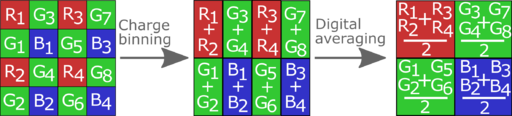
\includegraphics[width=0.6\textwidth]{./img/binning.png}
	\caption[GHF workflow]{\centering Use case of spatial binning for
	generalisation of raster.
	Source: \textless\url{https://web.stanford.edu}}
	\label{map_cz}
\end{figure} 
\paragraph{Spatial binning}
	 Spatial aggregation is  useful in summarizing big data to gain a meaningful
	view on map patterns. Spatial aggregation works by creating square bins of a
	user specified size.


	From shown\ref{map_eu} visualisation of Open Street Map it is hard to recognize any specific
		information. For classification  and visualisation this amount of data no
		desktop GIS tools is available. The possible approach use aggregation of data into bins, and
		visualises map of reasonable amount of data using desktop GIS.
		\begin{figure}[!htbp]
			\centering
			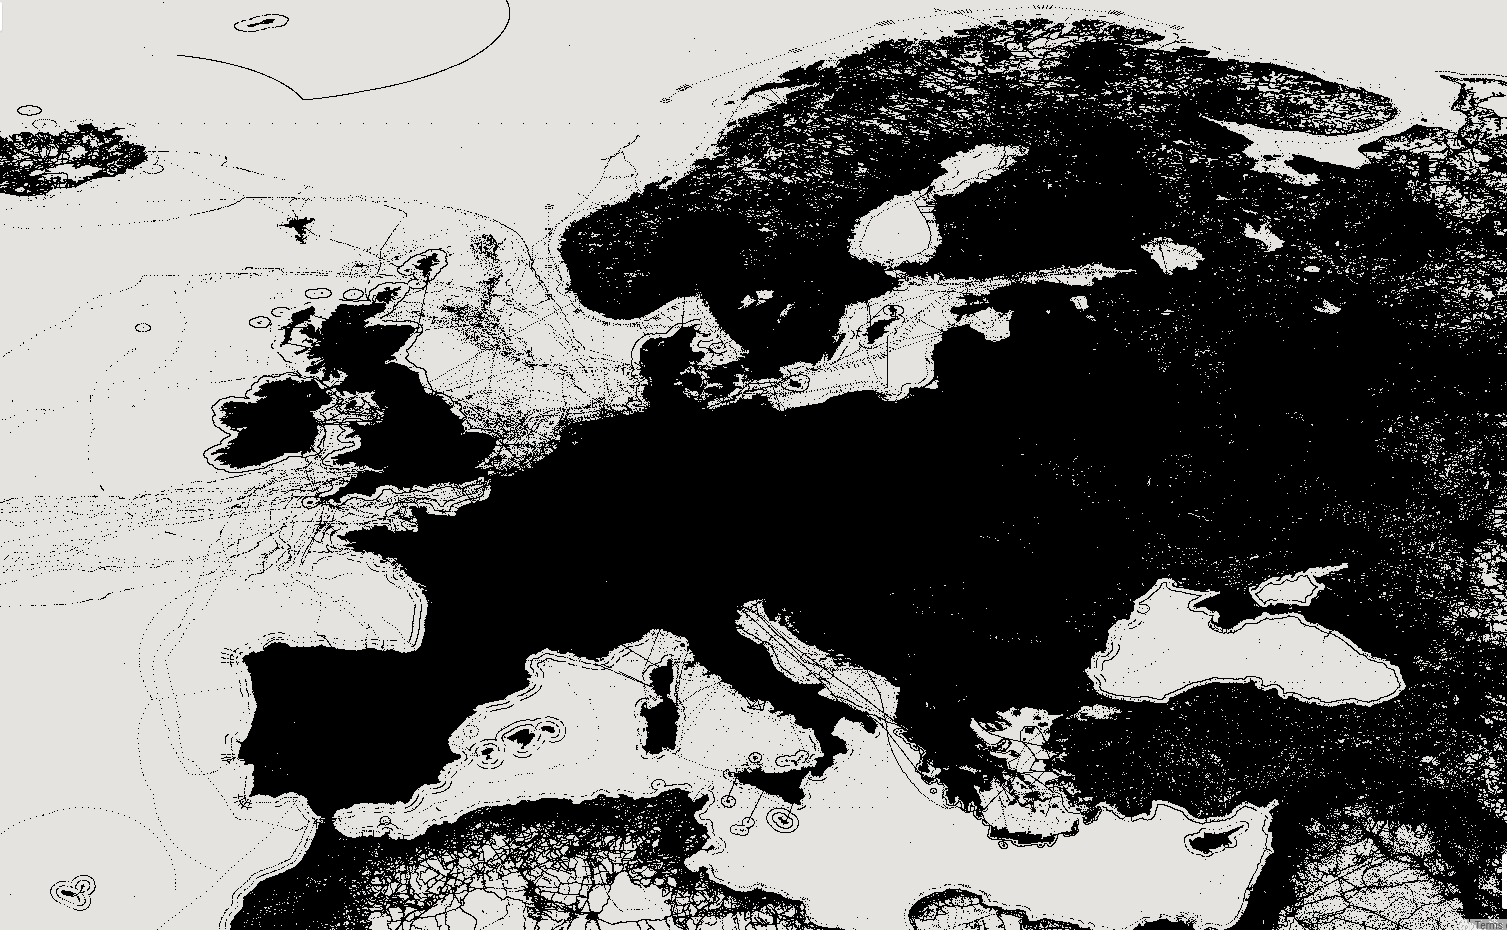
\includegraphics[width=0.8\textwidth]{./img/eu_all.png}
			\caption[GHF workflow]{\centering Snap shot of 1.3 billions of points from
			Open Street Map Planet dataset \newline
			Source: \textless\url{http://spatialhadoop.cs.umn.edu/datasets/osm2/all_nodes.pyramid/}}
			\label{map_eu}
		\end{figure}
	
Let's create table for output of spatial binning. Notice, that for serialization of data is used library of ESRI framework. 
	The last line consists from class for replacing key by null before feeding the writer of output format.
\begin{footnotesize}
	\begin{lstlisting}[style=python]
# Creation of table for results of binning
CREATE TABLE europe_agg2014(area BINARY, count DOUBLE, bin_id BIGINT)
ROW FORMAT SERDE 'com.esri.hadoop.hive.serde.JsonSerde'              
STORED AS INPUTFORMAT 'com.seri.json.hadoop.UnenclosedJsonInputFormat'
OUTPUTFORMAT 'org.apache.hadoop.hive.ql.io.HiveIgnoreKeyTextOutputFormat';
		\end{lstlisting}
	\end{footnotesize}
	
	In table named europe\_agg2011 there will be stored result of spatial binning of points contribution between June 2010 and June 2011.
	Analogically creation of table within GHF is developed module \textit{hd.hive.json.table}
\begin{footnotesize}
	\begin{lstlisting}[style=python]
# Creation of table using  GHF
hive.json.table driver=hiveserver2
                   table=europe_agg2014
                   attributes="area BINARY, count DOUBLE, bin_id BIGINT"
                   serde=com.ESRI.hadoop.hive.serde.JsonSerde
                   outformat=org.apache.hadoop.hive.ql.io.HiveIgnoreKeyTextOutputFormat
                   stored=com.ESRI.json.hadoop.UnenclosedJsonInputFormat
                   -e -d
	\end{lstlisting}
\end{footnotesize}
	As has been created table for results, similarly have been created tables for each year between 
	the beginning of project till 2014, so 2006,2007.. 2014. 
	
	
	The next and last stem is execution of spatial query for binning. The command firstly create bin(ST\_Bin) for each point. Bin is not special datatype but is represented as polygon simple feature which is in ESRI word called ring or \textit{esriGeometryRing}. Than, function \textit{ST\_BinEnvelope} create uniform  cells-based polygon of defined size. Actually, the function returning bin envelope for given bin ID or point. The \textit{GROUP BY} statements provide aggregation.
\begin{footnotesize}
	\begin{lstlisting}[style=python]
#Spatial binning for given time interval
FROM (SELECT ST_Bin(0.2, ST_Point(lon,lat)) bin_id, time 
FROM europe 
WHERE time > '2013-06-00 00:00:00' AND time < '2014-06-00 00:00:00') bins
INSERT OVERWRITE TABLE europe_agg2014
SELECT ST_BinEnvelope(0.2, bin_id) shape, COUNT(*) count, bin_id 
GROUP BY bin_id;
	\end{lstlisting}
\end{footnotesize}
	Firstly, are created bins which are within the time interval and than are aggregate.
	The size of bin was defined as 0.2 degrees which is approximately 22km.
	
	The execution of query can be made from \textit{hiveserver2} command line or using \textit{hd.hive.execute}. 
	
	\paragraph{Transfer data to GRASS}
	If Map and Reduce processing finish. Data are stored in table \textit{europe\_agg2014}, 
	which is located in hdfs://user/hive/warehouse/europe\_agg2014. The folder consists several
	files with 000000\_0, 000001\_0 etc. Each file represents data block of HDFS.  

\begin{footnotesize}
	\begin{lstlisting}[style=python]
#Spatial binning for given time interval
hd.hdfs.out.vector.py driver=webhdfs
                      out=europe_agg2013 
                      attributes='count int,bin_id int' 
                      table=europe_agg2013
	\end{lstlisting}
\end{footnotesize}
	Using module \textit{hd.hdfs.to.vector} is provided transfer of data from DataNodes to local system. Data are temporary stored in temporal directory of GRASS. After transfer of data, each 
	map block is converted to ESRI GeoJSON and exported as native GRASS vector map. In addition is build and printed GRASS command for merging split blocks to a contiguous map. This task is not automatic due to size block variability  and further processing variation. Module allows two
	 ways how locate data on HDFS. For automate way is parameter \textit{table}. For this approach, user
	 define name of table and hive driver\footnote{using hd.connect must be set connection to Hive} using Hql query 'describe formatted' recognize location of table in HDFS.
	 Second way is to define HDFS path manually using parameter \textit{hdfs}
	
	Now, the spatial analyses using GHF and ESRI Spatial Framework for Hadoop is done and result can be processed within GRASS GIS. In figures\ref{fig:outmap},\ref{fig:outmap1} is shown visualization aggregated points into bins.
	
	 In addition, using the same precess patter was aggregate all points for whole history of Open Street Map project on the area of Europe. Thus, approximately 1.3 billions  of points  to bin  resolution 0.1 degree. The map us in attachment\ref{open_street_agg_all}. 
	
	
	
	\paragraph{Summary of usage GHF}
	GRASS Hadoop framework
		
		
		
		
		\begin{figure}[htp]
		  \centering
	
	  \subfloat[2006-2007]{\label{figur:1}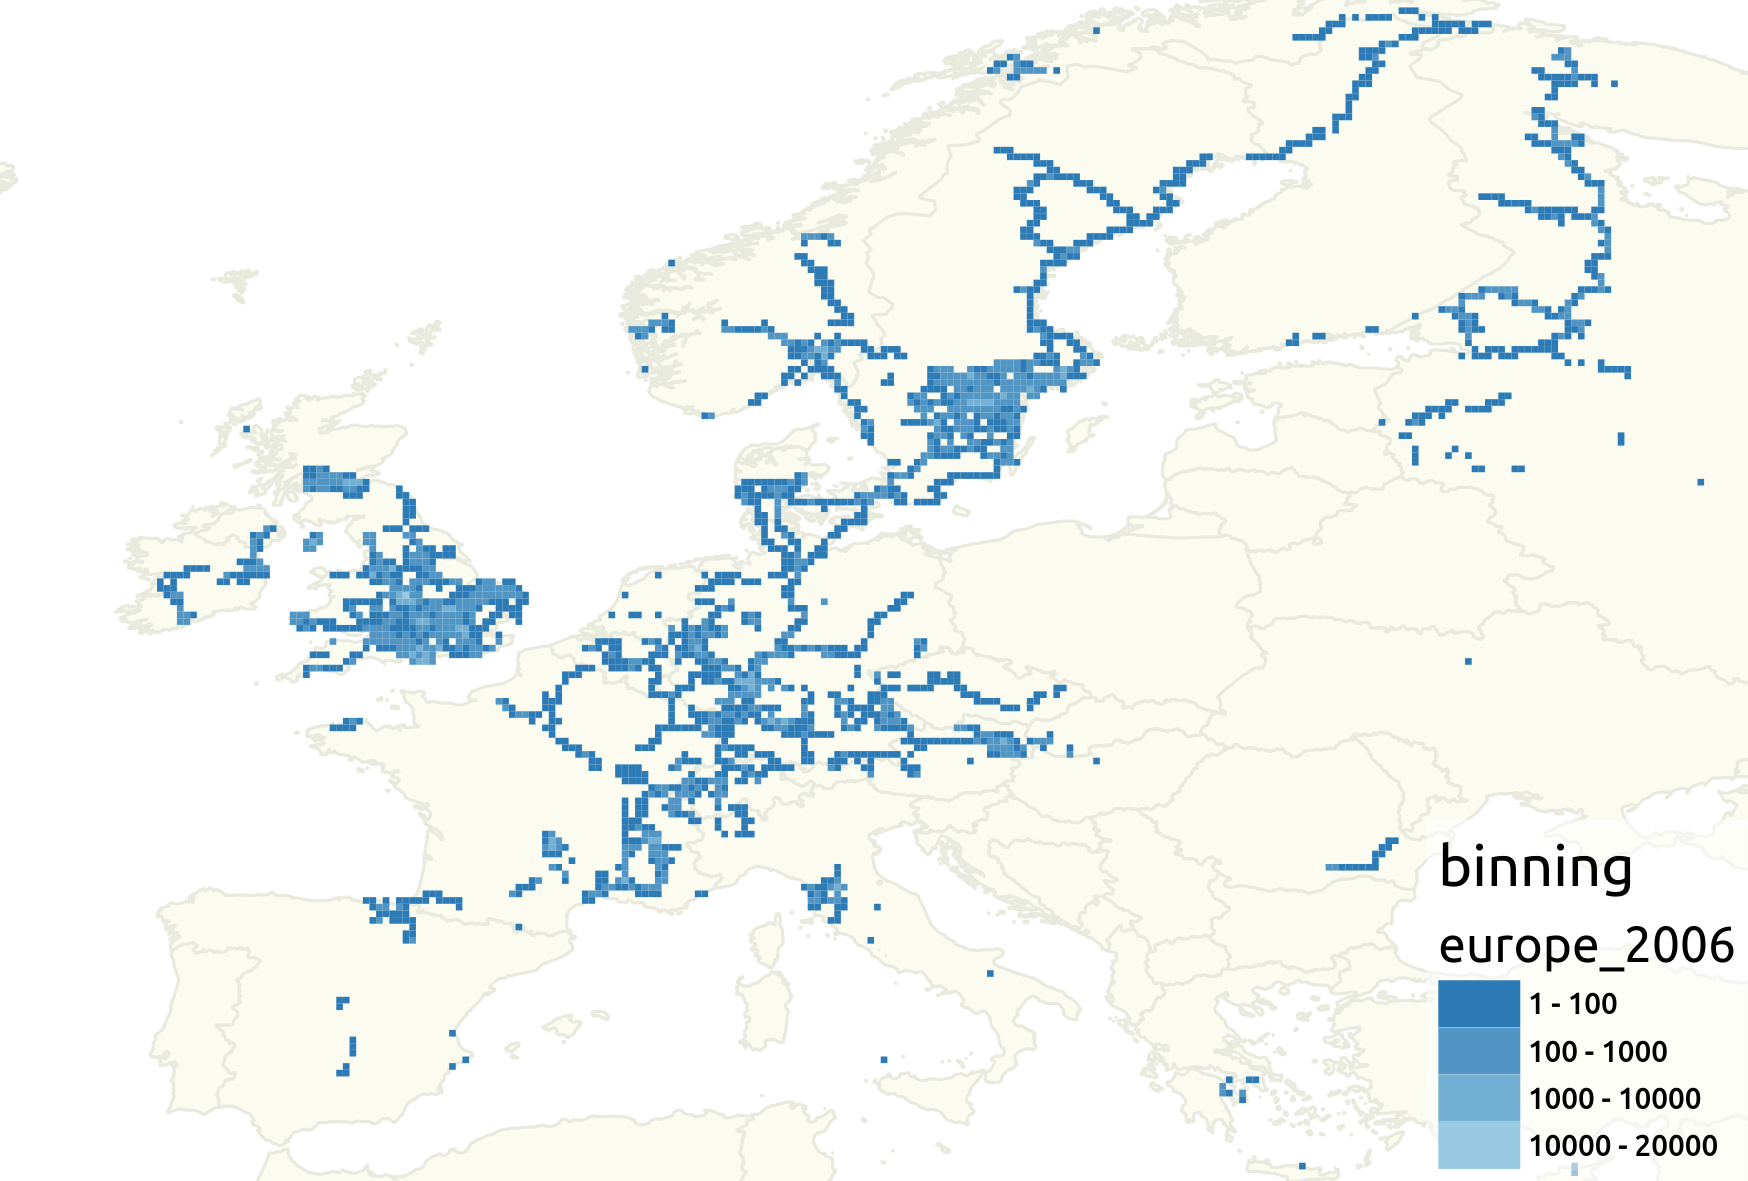
\includegraphics[width=0.5\textwidth]{./img/osm/2006.png}}
		  \subfloat[2007-2008]{\label{figur:2}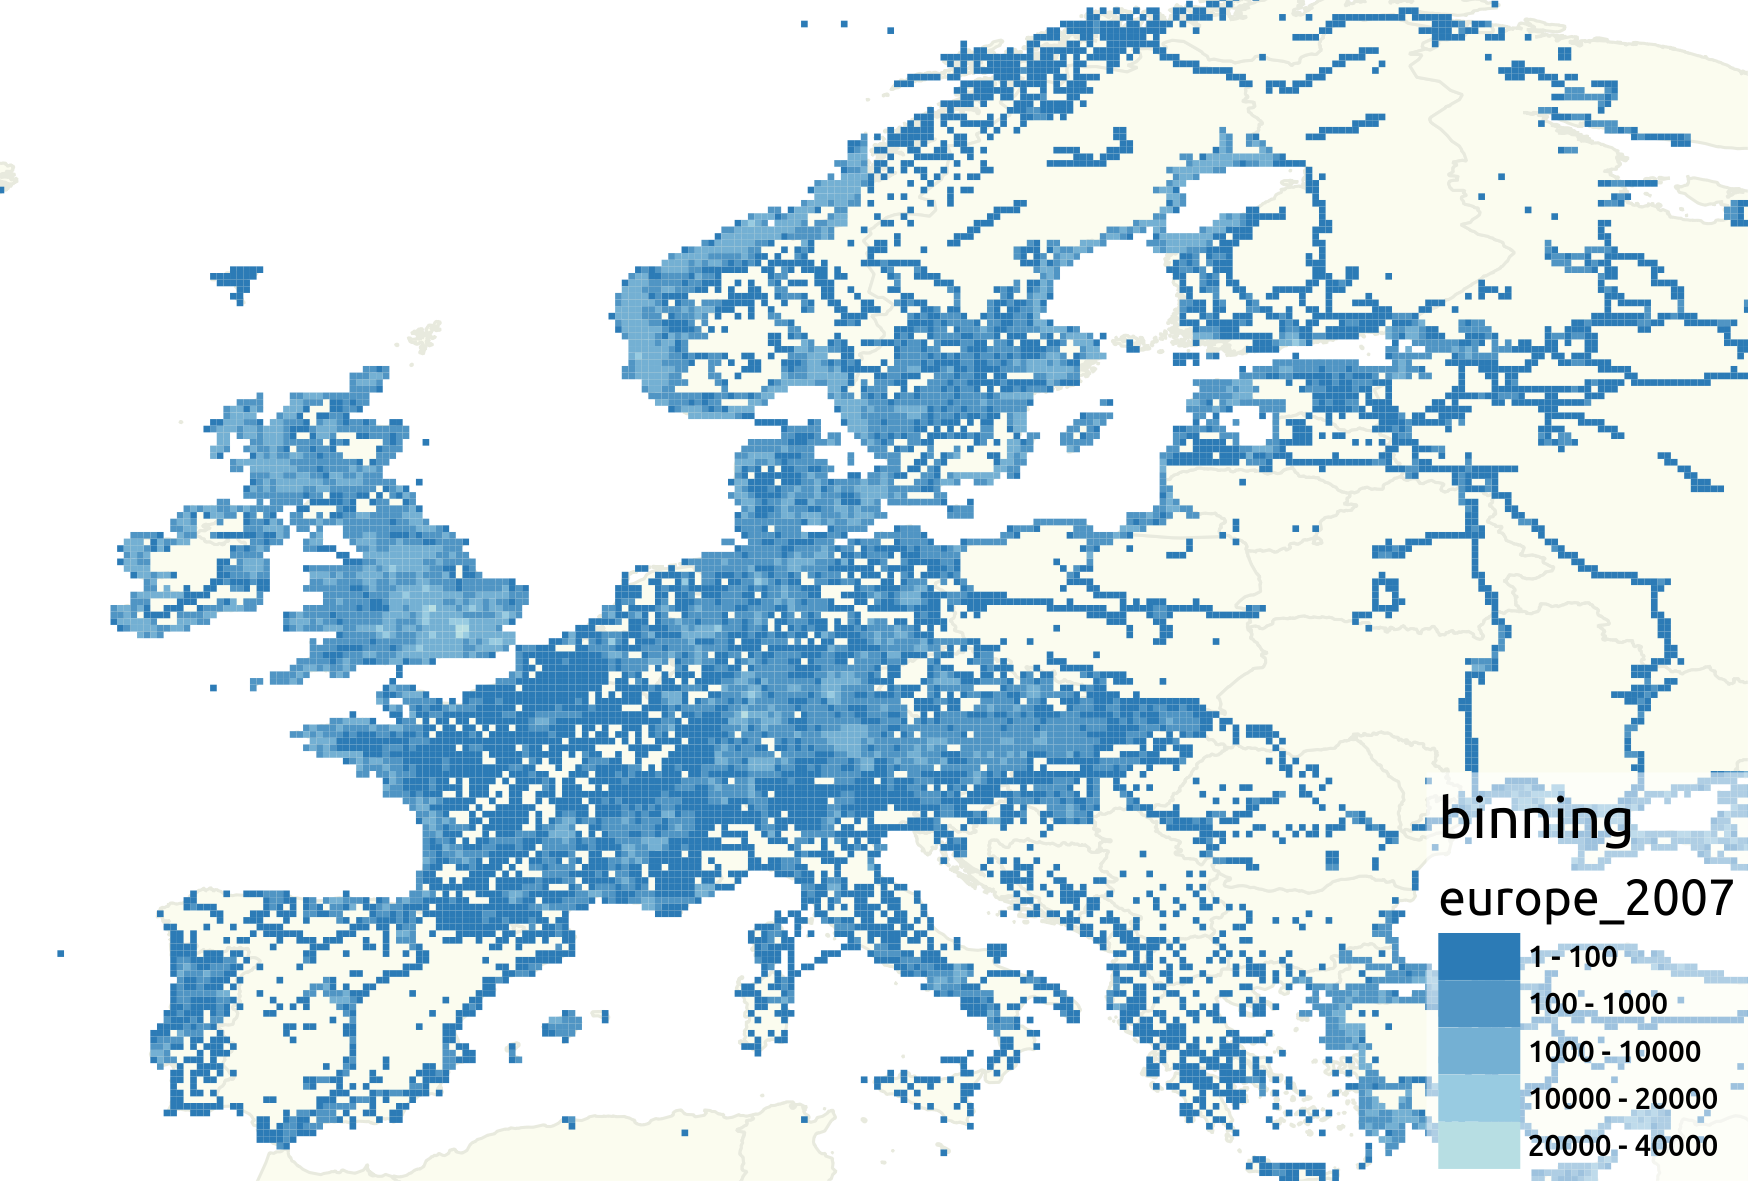
\includegraphics[width=0.5\textwidth]{./img/osm/2007.png}}
		  \\
			\label{figur}\caption{Aggregation of OSM points for particulars 1 year interval. 
			The resolution of spatial binning is 0.2 degree (approx 20km). The source OSM map consists of 1.3 billions of points.
			}
			\label{fig:outmap}
		\end{figure}
	
	\begin{figure}[htp]
	  \centering
	  \subfloat[2009-2009]{\label{figur:3}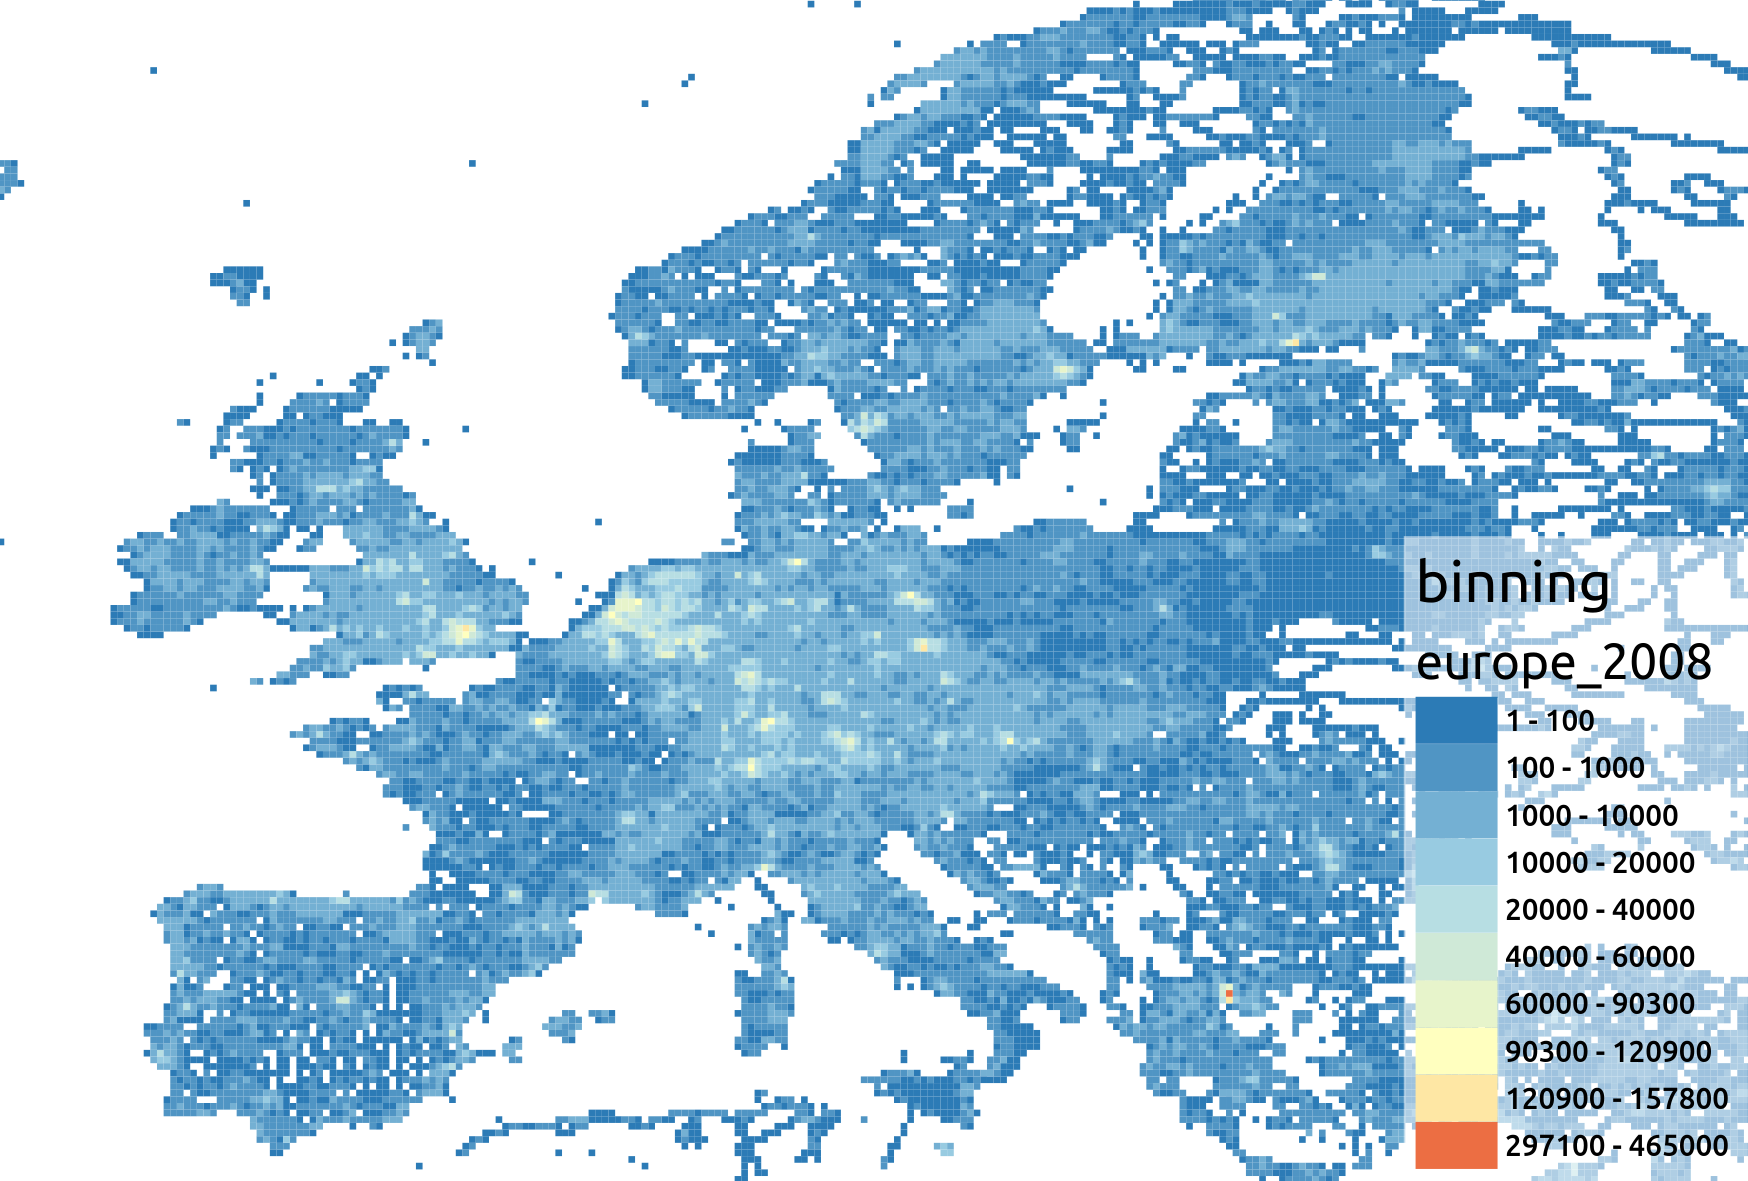
\includegraphics[width=0.5\textwidth]{./img/osm/2008.png}}
	   \subfloat[2009-2010]{\label{figur:4}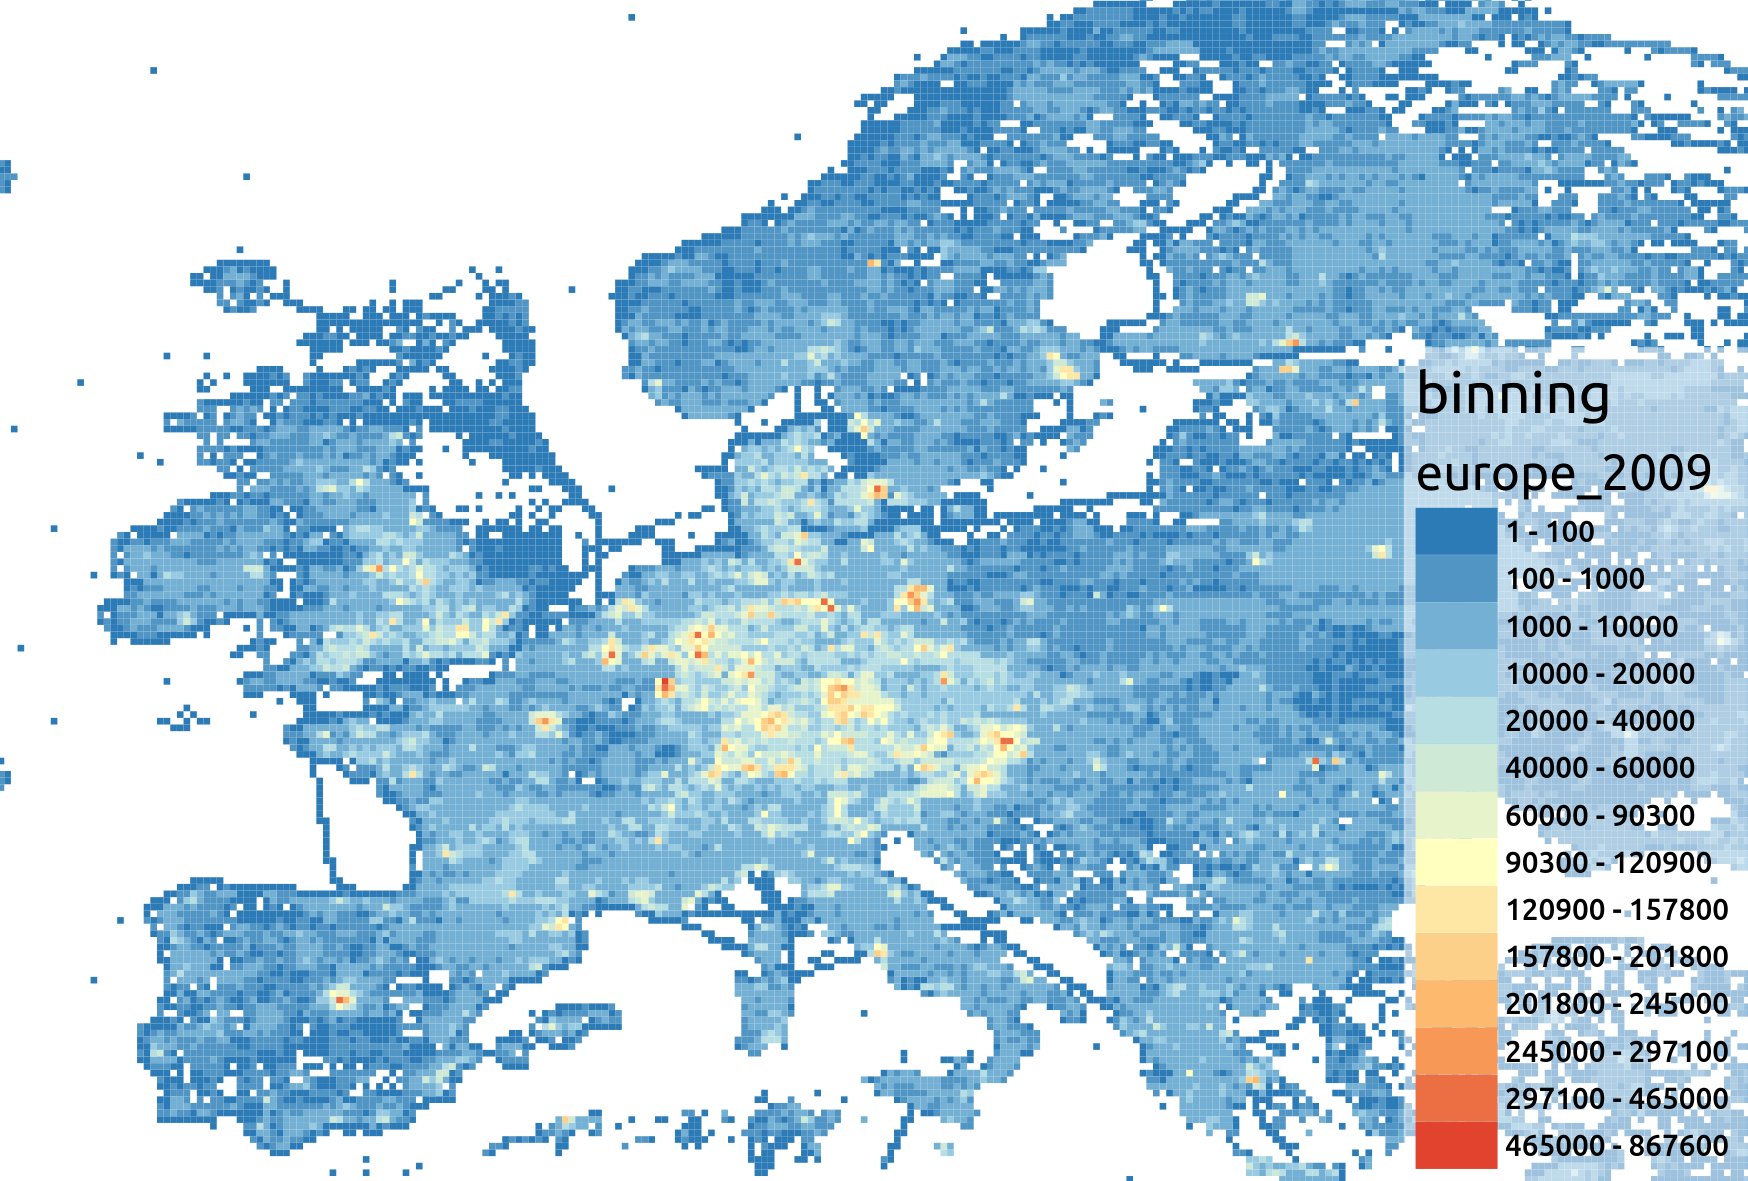
\includegraphics[width=0.5\textwidth]{./img/osm/2009.png}}
	   \\
	  \subfloat[2010-2011]{\label{figur:5}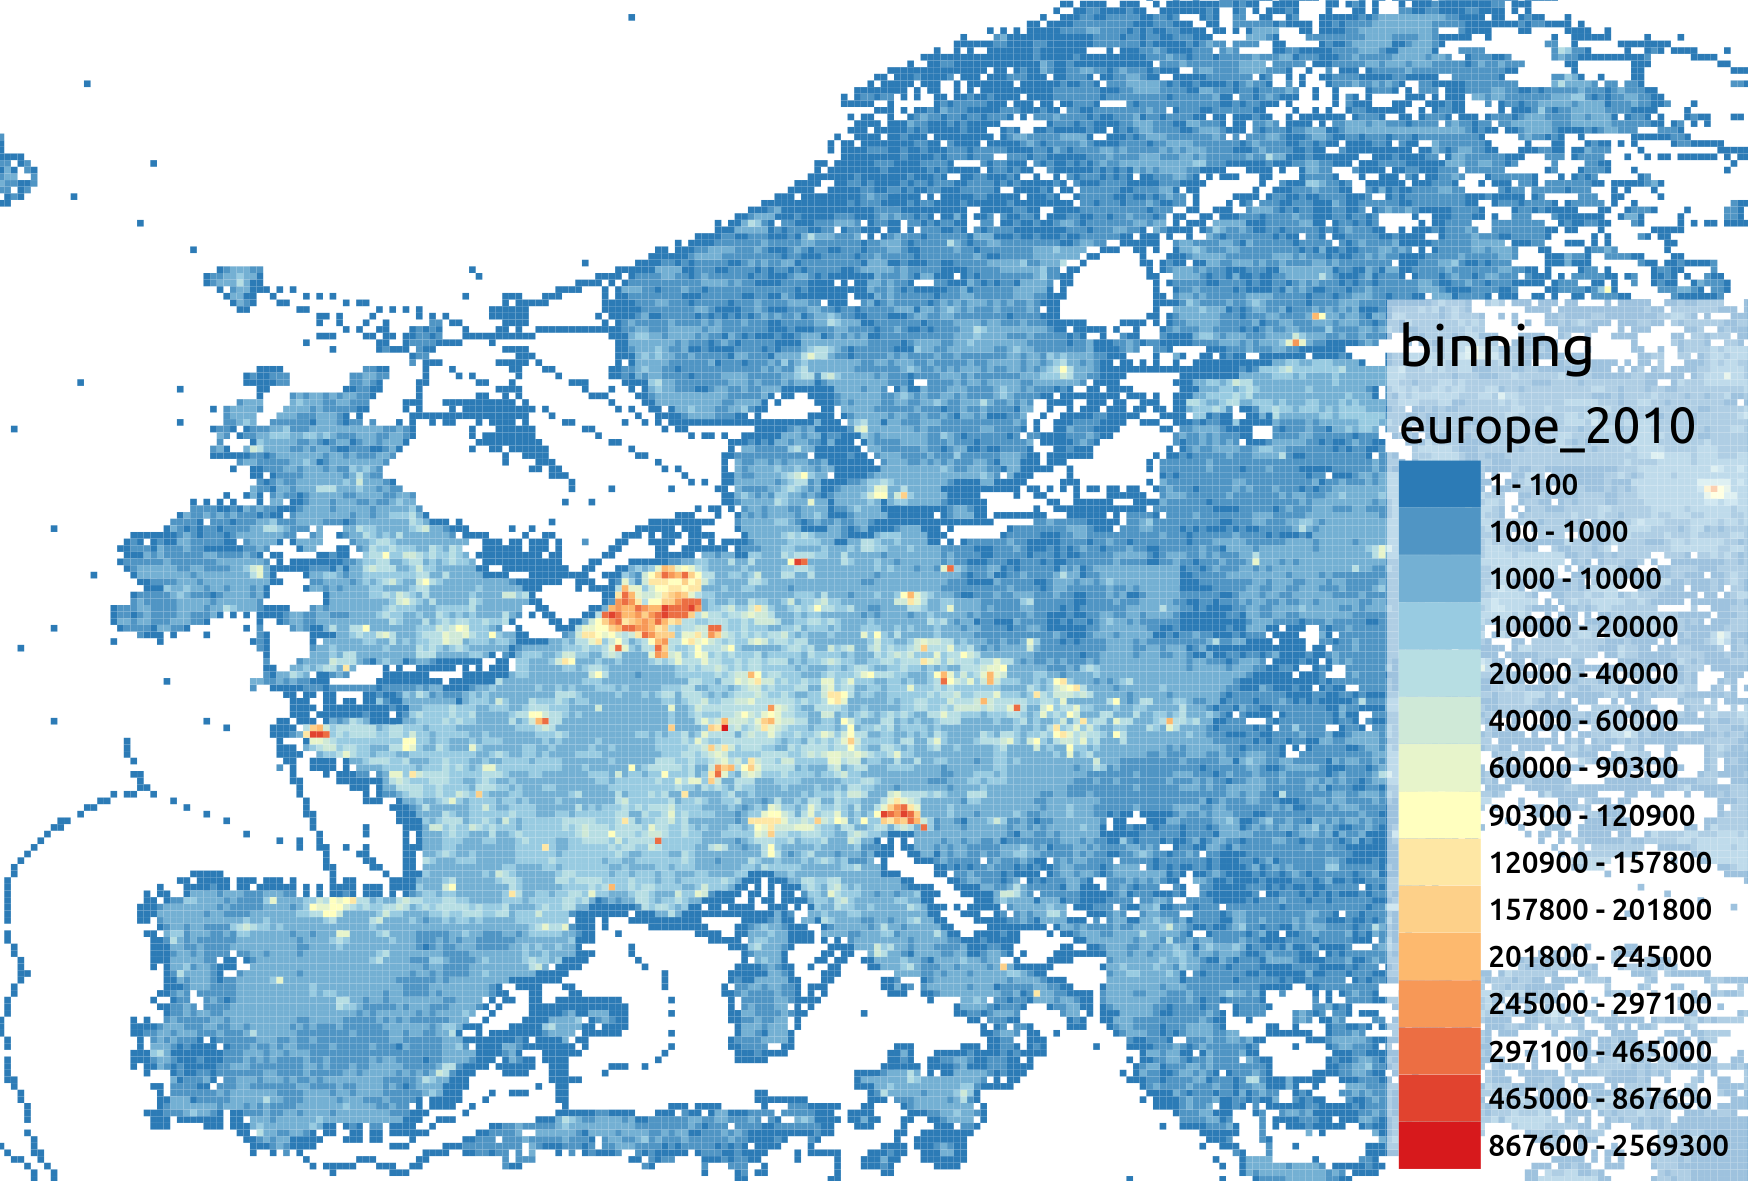
\includegraphics[width=0.5\textwidth]{./img/osm/2010.png}}
	   \subfloat[2011-2012]{\label{figur:6}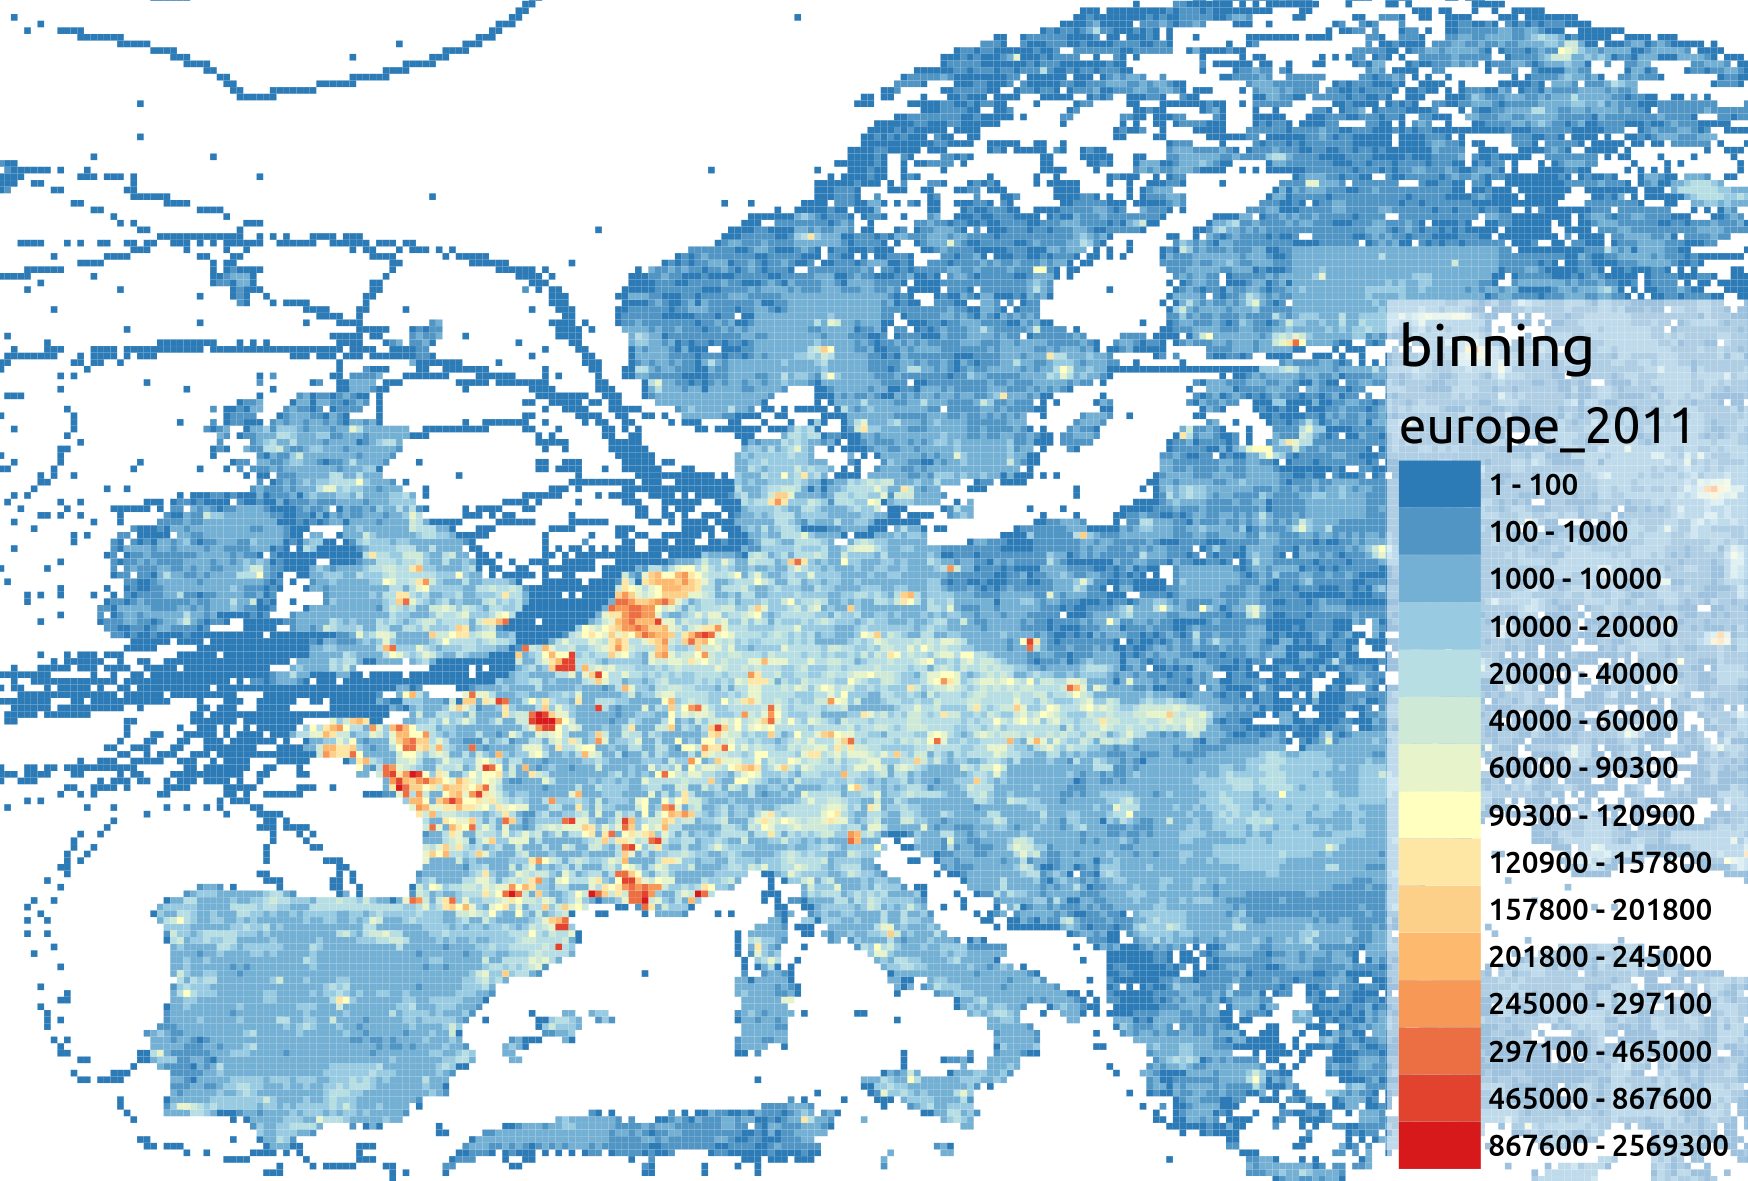
\includegraphics[width=0.5\textwidth]{./img/osm/2011.png}}
	   
	   	  \subfloat[2012-2013]{\label{figur:1}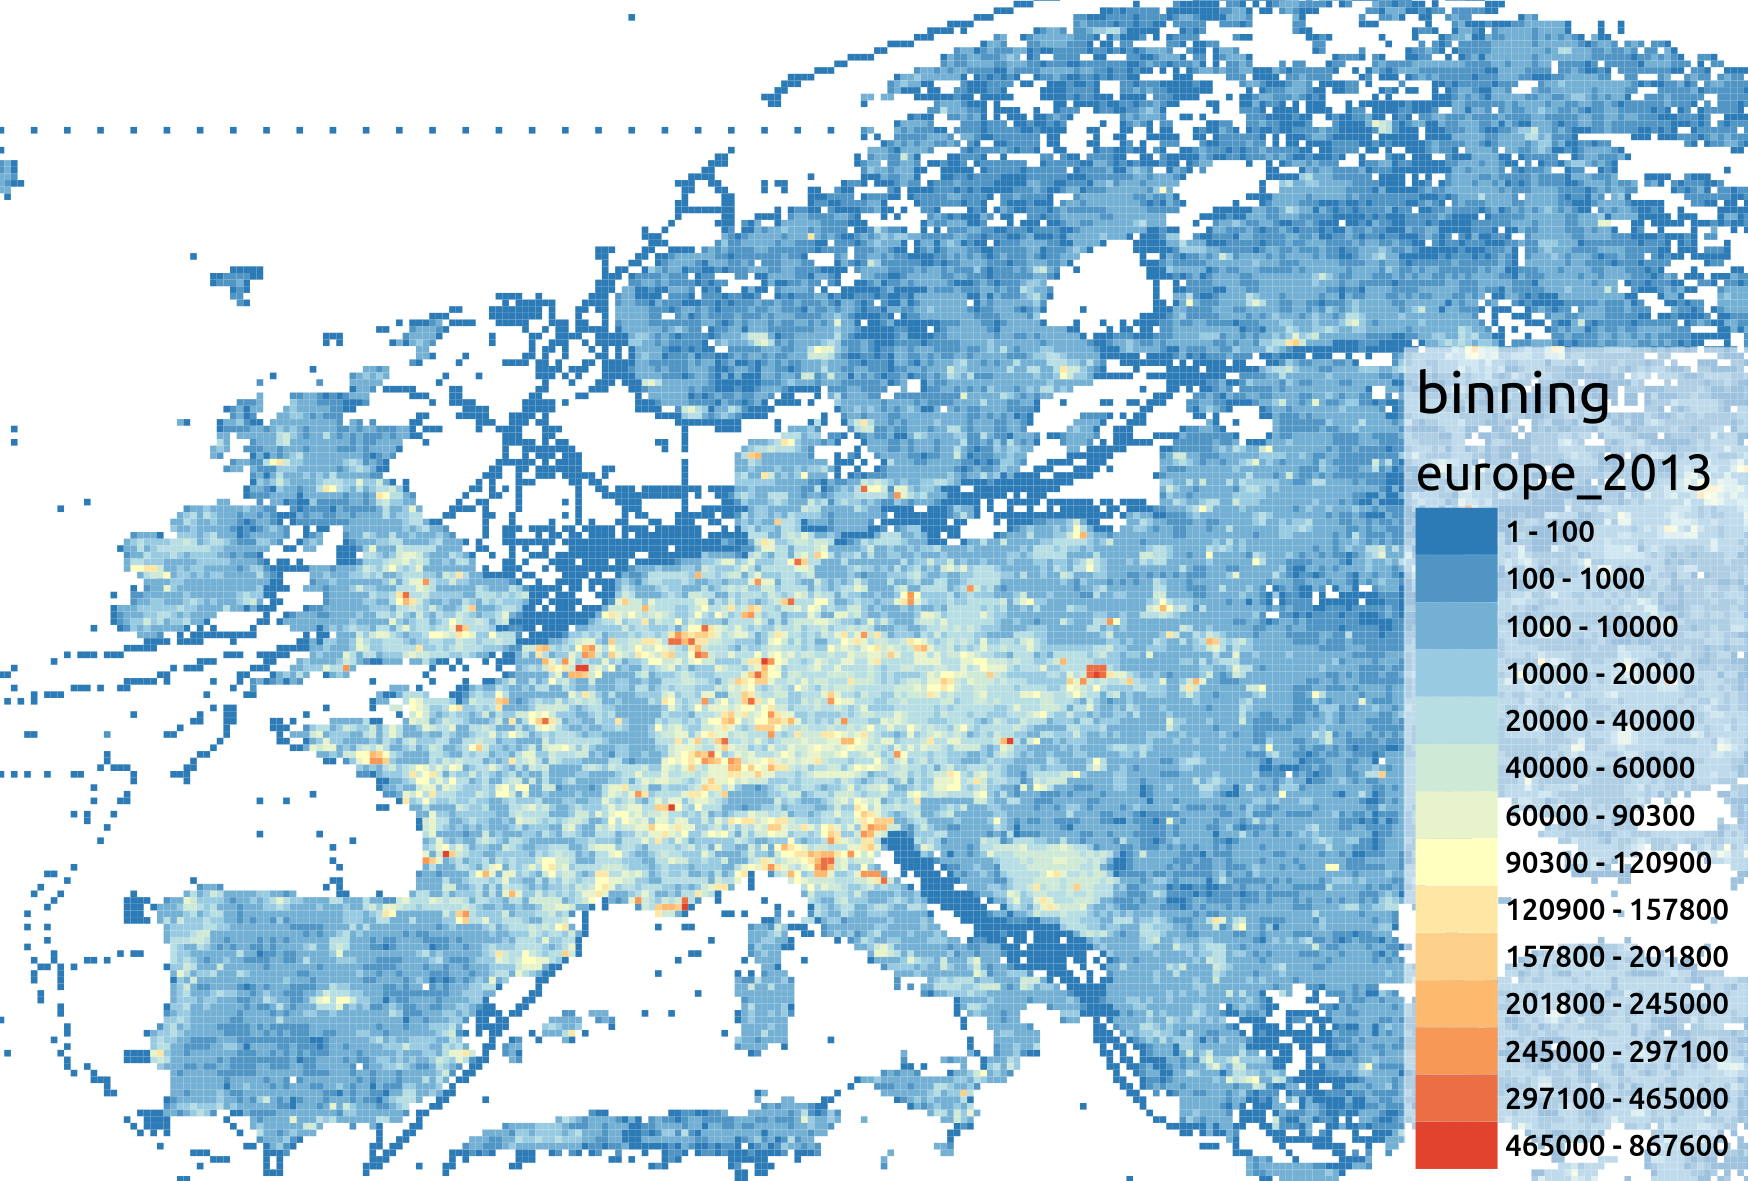
\includegraphics[width=0.5\textwidth]{./img/osm/2013.png}}
	   	  \subfloat[2013-2014]{\label{figur:2}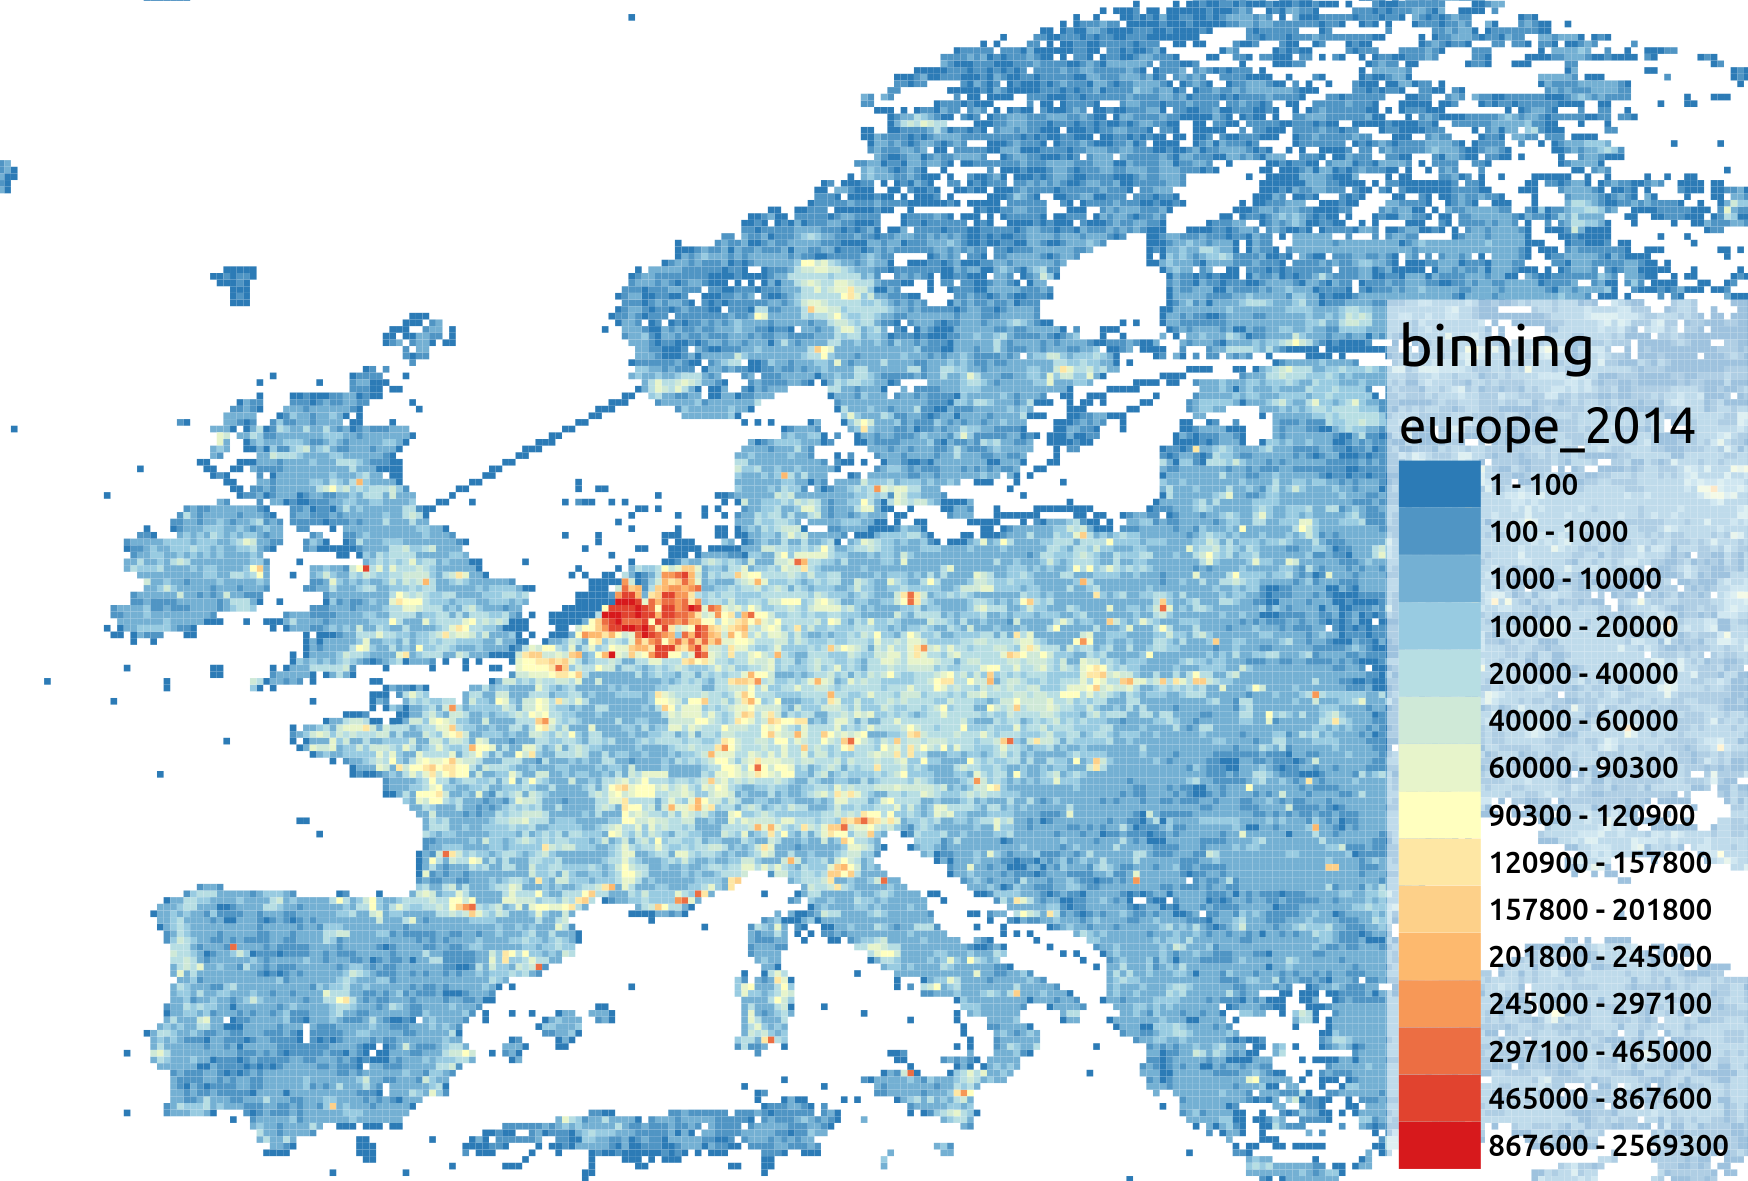
\includegraphics[width=0.5\textwidth]{./img/osm/2014.png}}
		\label{figur}\caption{Aggregation of OSM points for particulars 1 year interval. 
		The resolution of spatial binning is 0.2 degree (approx 20km). The source OSM map consists of 1.3 billions of points.
		}
		\label{fig:outmap1}
	\end{figure}
	

	
	\newpage
	\section{Conclusion}
	
	The first part of work introduced essentials and features of Hadoop design and its
	components. The following discussion aims on problems of spatial libraries coupled with Hadoop. 
	The second chapter expands the theoretical principles by the application in practice and describes 
	functionality, implementation and usage of developed GRASS Hadoop framework in detail.
	First chapter briefly introduced Hadoop ecosystem and its main components: distributed filesystem, layer for parallel processing - MapReduce and architecture of Hadoop server components. Thereafter, detailed analysis of the
	functionality and implementation strategy of spatial libraries for Hadoop is
	done. Following discussion deals with the challenges connected to spatial
	processing using MapReduce/HDFS and walk through particulars solutions for each
	library. The rest of the first part overviews Google Cloud Platform, 
	especially services for cluster hosting.
	
	Experiment framework consists processing workflow with included description of 
	implemented tools in detail. As the first step in the workflow tasks nascent 
	within the setup of working environment and Hadoop configuration are described. Thus, 
	set up environment for developing Hadoop/Hive client application. In addition, 
	the configuration of  cluster for performance of spatial processing is also described.
	The next section introduces functionality of developed framework for GRASS and overview 
	implementation design.  
	
	\subsection*{Contribution}
	The main goal of the work was design and implement processing workflow for
	interaction  between  Hadoop and GRASS GIS. Especially brings native access to
	distributed filesystem and data warehouse Hive within GRASS. This combination
	allows to use external libraries for parallel spatial processing. 
	
	As experiment within work GRASS Hadoop framework(GHF) has been developed.
	The package includes several GRASS command line modules for interaction between
	Hadoop and Hive. The full pack of modules simplified and automated the
	processing workflow. Therefore conversion data to serialized format, provides
	transaction of data to distributed filesystem and load data to Hive data
	warehouse which supports two spatial libraries. The result of highly demanding 
	performance of spatial analysis by the GRASS Hadoop Framework provides transfer of
	results to local filesystem and conversion to the native GRASS vector map. 
	
	The use case shown GRASS Hadoop Framework in use. The Europe extraction of OSM Planet dataset consisting 1.3 billions of point
	 has been processed on Hadoop using GRASS native interface. The developed framework
	 met expectations to be user friendly and effective tool.
	
	\subsection*{Further work}
	Package GRASS Hadoop Framework to compare with ESRI Hadoop GP Toolbox
	provide in many ways same functionality, even more, like Hive support or manager for connections. On the other hand, ESRI supports executing Apache Oozie workflow for Hadoop even  it is with several limitation. The further enhancement of GHF is supposed to be implementation of Oozie workflow support.
	
	The design of GHF respecting design layers based on interfaces hierarchy. The fact that core API is implemented independently on GRASS  and middle interface is dependent only partly is allowed to bring developed code into another GIS project. In field of open source free GIS open room for developing similar framework for Quantum GIS(QGis). Due to design, this task will consists only implementation of GUI interface(QtGUI) and minor refracting of part of code which is connected to GRASS map conversion tools.

	 	\pagenumbering{gobble}
	
	
	\chapter*{}\stepcounter{chapter}\addcontentsline{toc}{chapter}{}
	
		\listoffigures
		 
		\listoftables
	
	

	\newpage
	\necislovana{Acronyms}
	\begin{acronym}
		\setlength{\parskip}{0ex}
		\setlength{\itemsep}{1ex}
		\acro{ACLs}{Access Control Lists}
		\acro{API}{Application Programming Interface}
		\acro{bdutil}{Command line script designed for managing}
		\acro{BOS}{Boundary optimized strip partitioning}
		\acro{BSP}{Binary split partitioning}
		\acro{IAM}{Identity and Access Management}
		\acro{CPU}{Central processing unit}
		\acro{CRC32C}{Cyclic redundancy check}
		\acro{CSV}{Comma-separated values}
		\acro{DNS}{Domain Name System}
		\acro{EMR}{Elastic Map Reduce}
		\acro{FG}{Fixed grid partitioning}
		\acro{GRASS}{Geographical Resources Analysis Support System}
		\acro{GCS}{Google Cloud Storage}
		\acro{GNU GPL}{GNU General Public License } 
		\acro{GHF}{GRASS Hadoop Framework}
		\acro{GIS}{Geographic information system}
		\acro{GIT}{Version control system that is widely used software development}
		\acro{GPL}{General Public License}
		\acro{GUI}{Graphical user interface}
		\acro{HC}{Hilbert curve partitioning}
		\acro{HDFS}{Hadoop Distributed File system}
		\acro{CLI}{Comand line interface}
		\acro{HttpFS}{HttpFS is a server that provides a REST HTTP gateway}
		\acro{IAM}{Identity and Access Management}
		\acro{IP}{Internet Protocol address}
		\acro{JDBC}{Java Database Connectivity}
		\acro{JSON}{JavaScript Object Notation}
		\acro{LISP}{Locator/Identifier Separation Protocol}
		\acro{MBB}{Minimal Bounding Box}
		\acro{MBR}{Minimal Bounding Rectangle}
		\acro{MPI}{Message Passing Interface}
		\acro{MWL}{Microwave links}
		\acro{NoSQL}{COM Structured Storage}
		\acro{OGC}{Open Geospatial Consorcium}
		\acro{ORM}{SQL	Object-relational mapping}
		\acro{PD}{Extra persistent disk}
		\acro{pip}{Python Package Index}
		\acro{POSIX}{Portable Operating System Interface}
		\acro{RDBMS}{Relational database management system}
		\acro{REST API}{Representational state transfer  Application Programming Interface}
		\acro{SerDe}{Serializer and Deserializer}
		\acro{SLC}{Strip partitioning}
		\acro{SQL}{Structured Query Language}
		\acro{SSH}{Secure Shell}
		\acro{STR}{Sort-tile-recursive partitioning}
		\acro{TBB}{Threading Building Blocks}
		\acro{UDF}{Universal Disk Format}
		\acro{URI}{Uniform Resource Identifier }
		\acro{URL}{Uniform Resource Locator}
		\acro{VM}{Virtual machine}
		\acro{WKB}{Well known binary}
		\acro{XML}{Extensible Markup Language}
		\acro{YARN}{yet another resource negotiator}
	\end{acronym}
	
	
	
	
	\newpage
	\renewcommand\baselinestretch{1.2}
	\selectfont
	\renewcommand{\refname}{References}
	\phantomsection
	\addcontentsline{toc}{section}{ \refname}
	
	\begin{thebibliography}{99}
		\label{References}
		
		\bibitem{digit_universe}
		John Gantz, David Reinsel. \textit{THE DIGITAL UNIVERSE IN 2020: Big Data,
		Bigger Digital Shadow and Biggest Growth in
		the Far East}, December 2012
\textless\url{http://www.emc.com/collateral/analyst-reports/idc-the-digital-universe-in-2020.pdf}
		
		\bibitem{hadoop_definitive}
		WHITE, Tom. \textit{Hadoop: the definitive guide. Fourth edition.} Beijing:
		O'Reilly, 2015. ISBN 14-919-0163-2.
		
		\bibitem{kerberos}
		NEUMAN, B.C. a T. TS'O. \textit{Kerberos. IEEE Communications Magazine}. 1994,
		32(9). DOI: 10.1109/35.312841. ISSN 0163-6804.  URL:
\textless\url{http://ieeexplore.ieee.org/lpdocs/epic03/wrapper.htm?arnumber=312841}

		\bibitem{spatial_join}
		JACOX, Edwin H. a Hanan SAMET. \textit{Spatial join techniques}. ACM
		Transactions on Database Systems. 2007, 32(1), 1-5. DOI:
		10.1145/1206049.1206056. ISSN 03625915. URL:
		\textless\url{http://portal.acm.org/citation.cfm?doid=1206049.1206056}
		
		\bibitem{partitioning}
		Ablimit Aji, Vo Hoang, Fusheng Wang \textit{Effective Spatial Data
		Partitioning
			for Scalable Query Processing} 2015/9/3,
		Journal: arXiv preprint arXiv:1509.00910
		\textless\url{http://arxiv.org/pdf/1509.00910}
		
		\bibitem{spatial_skew}
		Ray, Suprio, et al. \textit{Skew-resistant parallel in-memory spatial join.}
		Proceedings of the 26th International Conference on Scientific and Statistical
		Database Management. ACM, 2014.
		
		\bibitem{spatial_join2}
		YOU, Simin, Jianting ZHANG a Le GRUENWALD. \textit{Large-scale spatial join
			query processing in Cloud.} 2015 31st IEEE International Conference on Data
		Engineering Workshops. IEEE, 2015, , 34-41. DOI: 10.1109/ICDEW.2015.7129541.
		ISBN 978-1-4799-8442-8. URL:
\textless\url{http://ieeexplore.ieee.org/lpdocs/epic03/wrapper.htm?arnumber=7129541}
		
		\bibitem{covex_hull}
		GOMES, Abel J.P. A \textit{Total Order Heuristic-Based Convex Hull Algorithm
for
			Points in the Plane. Computer-Aided Design.} 2016, 70, 153-160. DOI:
		10.1016/j.cad.2015.07.013. ISSN 00104485.  URL:
		\textless\url{http://linkinghub.elsevier.com/retrieve/pii/S001044851500113X}
		
		\bibitem{omp}
		Wirz, Alexander, Björn Knafla, and Claudia Leopold. \textit{Comparison of
			Spatial Data Structures in OpenMP-Parallelized Steering.} HIGH PERFORMANCE
		COMPUTING  SIMULATION (HPCS 2008) (2008): 31.
		
		\bibitem{multi_cpu}
		ZHANG, Jianting, Simin YOU a Le GRUENWALD. \textit{Parallel online spatial and
			temporal aggregations on multi-core CPUs and many-core GPUs.} Information
		Systems. 2014, 44, 134-154. DOI: 10.1016/j.is.2014.01.005. ISSN 03064379.URL: 
		\textless\url{http://linkinghub.elsevier.com/retrieve/pii/S0306437914000234}
		
		
		\bibitem{hadoopGIS}
		AJI, Ablimit, Fusheng WANG, Hoang VO, Rubao LEE, Qiaoling LIU, Xiaodong ZHANG
a
		Joel SALTZ. \textit{Hadoop GIS:A High Performance Spatial Data Warehousing
			System over MapReduce.} 2013, 6(11), 1009-1020. DOI:
10.14778/2536222.2536227.
		ISSN 21508097.  URL: 
		\textless\url{http://dl.acm.org/citation.cfm?doid=2536222.2536227}
		
		\bibitem{spatialhadoop}
		ELDAWY, Ahmed a Mohamed F. MOKBEL. \textit{SpatialHadoop: A MapReduce
framework
			for spatial data.} DOI: 10.1109/ICDE.2015.7113382. ISBN
		10.1109/ICDE.2015.7113382. URL: 
\textless\url{http://ieeexplore.ieee.org/lpdocs/epic03/wrapper.htm?arnumber=7113382}
		
		\bibitem{ESRI_indexing}
		WHITMAN, Randall T., Michael B. PARK, Sarah M. AMBROSE a Erik G. HOEL.
		\textit{Spatial indexing and analytics on Hadoop.} Proceedings of the 22nd ACM
		SIGSPATIAL International Conference on Advances in Geographic Information
		Systems - SIGSPATIAL '14. New York, New York, USA: ACM Press, 2014, , 73-82.
		DOI: 10.1145/2666310.2666387. ISBN 9781450331319. URL: 
		\textless\url{http://dl.acm.org/citation.cfm?doid=2666310.2666387}
		
		\bibitem{spatial_indexing}
		FOX, Anthony, Chris EICHELBERGER, James HUGHES a Skylar LYON.
		\textit{Spatio-temporal indexing in non-relational distributed databases.}
2013
		IEEE International Conference on Big Data. IEEE, 2013, , 291-299. DOI:
		10.1109/BigData.2013.6691586. ISBN 978-1-4799-1293-3. URL: 
	
\textless\url{http://ieeexplore.ieee.org/lpdocs/epic03/wrapper.htm?arnumber=6691586}
		
		\bibitem{google_fs}
		GHEMAWAT, Sanjay, Howard GOBIOFF a Shun-Tak LEUNG. \textit{The Google file
			system. ACM SIGOPS Operating Systems Review.} 2003, 37(5), 29-. DOI:
		10.1145/1165389.945450. ISSN 01635980.  URL: 
		\textless\url{http://portal.acm.org/citation.cfm?doid=1165389.945450}
		
		\bibitem{lisp}
		DEAN, Jeffrey a Sanjay GHEMAWAT. \textit{MapReduce: Simplified Data Processing
			on Large Clusters}  2008, 51(1), 107-. DOI: 10.1145/1327452.1327492. ISSN
		00010782. URL: 
	
\textless\url{http://static.googleusercontent.com/media/research.google.com/en//archive/mapreduce-osdi04.pdf}
		
		\bibitem{bp_krejci}
		Matej Krejci, Bachelor theses \textit{Analysis and vizualization of rainfall
data from microwave links using GIS} 
\textless\url{https://github.com/ctu-osgeorel-proj/bp-krejci-2014/blob/master/text/matej-krejci-bp-2014.pdf}
		%%%%%%% online
		\bibitem{permission}
		HDFS Permissions Guide, Apache Hadoop  [online]. [2016-05-06]. URL: 
\textless\url{https://hadoop.apache.org/docs/current/hadoop-project-dist/hadoop-hdfs/HdfsPermissionsGuide.html}
		
		\bibitem{ESRI_framework}
		GIS Tools for Hadoop. ESRI GitHub [online]. [2016-03-18]. URL: 
		\textless\url{http://esri.github.io/gis-tools-for-hadoop/}
		
		\bibitem{rest_api}
		WebHDFS REST API, Apache Hadoop  [online]. [2016-05-06]. URL: 
\textless\url{http://hadoop.apache.org/docs/current/hadoop-project-dist/hadoop-hdfs/WebHDFS.html#Append_to_a_File
		}
		
		\bibitem{amazon_emr}
		Amazon EMR. Amazon [online]. [2016-03-18]. 
		URL: \textless\url{https://aws.amazon.com/elasticmapreduce/}
		
		\bibitem{hadoop_web}
		Apache Hadoop main. Apache Hadoop [online]. [2016-03-18]. 
		URL: \textless\url{http://hadoop.apache.org/}
		
		\bibitem{nutch_web}
		Apache Nutch. Apache Hadoop [online]. [2016-03-18]. 
		URL: \textless\url{http://nutch.apache.org/#News
		}
		
		\bibitem{hadoop_news_web}
		Apache Hadoop news. Apache Hadoop [online]. [2016-03-18]. 
		URL: \textless\url{http://hadoop.apache.org/index.html#News}
		
		
		\bibitem{hadoop_hdfs_web}
		Apache Hadoop news. Apache Hadoop [online]. [2016-03-18]. 
		URL: \textless\url{https://hadoop.apache.org/docs/r1.2.1/hdfs_design.html}
		
		
		\bibitem{hadoop_rack_web}
		Hadoop Rack Awareness. Apache Hadoop [online]. [2016-03-18]. 
		URL:
\textless\url{https://hadoop.apache.org/docs/r1.2.1/cluster_setup.html#Hadoop+Rack+Awareness}
		
		\bibitem{gc_product_services}
		Google Cloud, Home Page [online]. [2016-04-18]. 
		URL: \textless\url{https://cloud.google.com}
		
		
		\bibitem{gc_hadoop}
		Google Cloud, Hadoop Configuration [online]. [2016-04-18]. 
		URL:
	
\textless\url{https://cloud.google.com/hadoop/setting-up-a-hadoop-cluster#setupscripts}
		
		\bibitem{yarn}
		Apache Hadoop docs. Apache Hadoop [online]. [2016-05-18]. 
		URL:
\textless\url{https://hadoop.apache.org/docs/r2.7.1/hadoop-yarn/hadoop-yarn-site/YARN.html}
		
		\bibitem{hadoop}
		Apache Hadoop setting up Single cluster node, Apache Hadoop [online].
		[2016-05-18]. 
		URL:
\textless\url{https://hadoop.apache.org/docs/r2.7.1/hadoop-yarn/hadoop-yarn-site/YARN.html}
		
		
		\bibitem{ESRI_gtfp}
		Geoprocessing Tools for Hadoop, GitHub. [online]. [2016-04-18]. 
		URL: \textless\url{https://github.com/esri/geoprocessing-tools-for-hadoopl}
		
		\bibitem{protobuf}
		Protocol Buffers, Google Developers [online]. [2016-0-29]. 
		URL: \textless\url{https://developers.google.com/protocol-buffers/}
		
		\bibitem{snakebite}
		Snakebite documentation, Snakebite readthedocs [online]. [2016-04-29]. 
		URL: \textless\url{http://snakebite.readthedocs.io/en/latest/index.html}
		
		\bibitem{gcloud_dataproc}
		Cluster properties, Google Cloud Platform [online]. [2016-04-29]. 
		URL:
		\textless\url{https://cloud.google.com/dataproc/concepts/cluster-properties}
		
		
		\bibitem{airflow_diff}
		Airflow Apache incubator project. Diff file is included in the attachment
		\ref{airflow_dif}
		
		\bibitem{bining}
		Applications of Parallel Computers (CS 5220), \textit{Spatial binning and
hashing}, Bindel,  [2016-04-29]. 
\textless\url{http://www.cs.cornell.edu/~bindel/class/cs5220-f11/notes/spatial.pdf}
		
		\bibitem{ESRI_serde}
		JSON Formats, GitHub,  [2016-04-29]. 
		\textless\url{https://github.com/esri/spatial-framework-for-hadoop/wiki/JSON-Formats}	
		
		
	\end{thebibliography}
	
	

	
	\setcounter{footnote}{1}
	\newpage
	
	\appendix
	
	\renewcommand\thesection{\Alph{section}}
	
	
	
\newpage	
	\chapter*{Attachment}
\section{Attachment: Transformation of SQL to BigQuery}
		\paragraph{SQL data migration} Within project have been created several
buckets
		for storing exported data from SQL. Data captured by microwave operator
T-Mobile has been 
		described	in my bachelor theses\cite{bp_krejci}. 	Date are stored in relation
database 
		PostgreSQL and includes over $3e9$ rows. Due to big data characteristic has
bee	developed python\ref{pythonscr} %TODO
		script for exporting data in defined time interval. It protects a database
from overloading by queries for all rows in one	query. 
		
		As a machine for exporting, merging and uploading data to bucket was used VM
		instance from Google Compute engine.
		
		\begin{footnotesize}
			\begin{lstlisting}[style=mybash]
#create compute engine with 500 GB persistent disk
$ gcloud compute --project "spatial-hadoop" disks create "vmexport" --size "500"
\
--zone "europe-west1-b" --type "pd-standard" --image \
"/debian-cloud/backports-debian-7-wheezy-v20160418"
			\end{lstlisting}
		\end{footnotesize}
		
		Table public.record from mwdb database has been exported in time step one
week.
		The merge of each exported 
		csv files has been merged using Unix \textit{cat} command. The size of
exported
		table record is around 98 GB or 17 GB tarball.
		
		
		\begin{footnotesize}
			\begin{lstlisting}[style=mybash]
#create bucket 
$ gsutil mb -l EU gs://mwdata_export
#copy big file with slicing
$ gsutil -m -o GSUtil:parallel_composite_upload_threshold=100M cp \
mwdump.csv gs://mwdata_export/
			\end{lstlisting}
		\end{footnotesize}
		
		\paragraph{BigQuery} is a top performance service based on distributed
database. The main characteristics are petabyte scale, low cost and unnecessary
maintenance. BigQuery interface is
		similar to SQL databases, where queries are similar. BigQuery is accessible by
API in several language an allows programmatic way for controlling. The pricing
model is based on pay-as-you-go.
		
		Using BigQuery has been created table\ref{tab_rec} accordingly to columns in
CSV file. 
		\begin{table}[]
			\centering
			\begin{footnotesize}
			
			\begin{tabular}{@{}|l|l|l|@{}}
				\toprule
				column & datatype  & mode     \\ \midrule
				linkid & INTEGER   & REQUIRED \\ \midrule
				time   & TIMESTAMP & NULLABLE \\ \midrule
				rx     & FLOAT     & NULLABLE \\ \midrule
				tx     & FLOAT     & NULLABLE \\ \bottomrule
			\end{tabular}
			\caption{Table record}
			\label{tab_rec}
			\end{footnotesize}
		\end{table}
		
		Table has been queried by several queries, which had impact on slowing down
the performance of GRASS GIS module \textit{g.gui.mwprecip}, which is developed
within my bachelor theses. The queries was massively speed up. Below are few
comparison of queries on PosgreSQL database on \textit{geo102.fsv.cvut.cz} and
on BigQuery scalable engine.
	\begin{footnotesize}
		\begin{lstlisting}[style=python]
SELECT linkid, avg(rxpower) FROM record WHERE time >='2014-07-07 10:53:00'\
 AND  time<='2014-07-27 10:53:00% \
 group by linkid order by 1
		\end{lstlisting}
	\end{footnotesize}
\begin{itemize}
\item PostgreSQL: 206.8 second
\item BigQuery: 2.3 second
\end{itemize}
	\begin{footnotesize}
		\begin{lstlisting}[style=python]
SELECT min(time) FROM mw.record
		\end{lstlisting}
	\end{footnotesize}
\begin{itemize}
\item PostgreSQL: 2.3 millisecond (index on time)
\item BigQuery: 2.4 second
\end{itemize}
	\begin{footnotesize}
		\begin{lstlisting}[style=python]
select linkid,avg(rx-tx) as m from record group by linkid
		\end{lstlisting}
	\end{footnotesize}
\begin{itemize}
\item PostgreSQL: 91.5 minutes
\item BigQuery: 4.2 second
\end{itemize}
	

\newpage
\section{Attachment: Compilation Spatial Libraries}
\label{att:java}
	\paragraph{Compilation} Below are some important notes for compilation of used
%%%: maven jsi nekde vysvetloval v textu?
%OK
	libraries. Especially for compilation of libraries with Apache
Maven\footnote{Apache packaging system for Java \url{https://maven.apache.org/}}
profiles.
	
	Usage of ESRI Spatial Framework for Hadoop is dependent on package Geometry API
	Java. After cloning GIT repository with ESRI Spatial Framework for Hadoop the
	maven test after packaging can failed. According to issue tracker of the
	repository is suggested to skip tests.
	\begin{footnotesize}
		\begin{lstlisting}[style=python]
sudo mvn clean package -DskipTests 
		\end{lstlisting}
	\end{footnotesize}
	
	For packaging JsonSerde \footnotetext{Json SerDe for Hive
		\textless\url{https://github.com/rcongiu/Hive-JSON-Serde}}
	must be choose package profile. According documentation is clear that the
	profiles are set to Hadoop distribution project such a \textit{Cloudera} and
	\textit{HortonWorks}. Thus its not completely clear which profile should be
used
	for different Hadoop versions. 
	
	For using Hadoop 1.x on Google Cloud works profile for Cloudera 4 (CDH4)
	\begin{footnotesize}
		\begin{lstlisting}[style=python]
mvn -Pcdh4 clean package
		\end{lstlisting}
	\end{footnotesize}
	For building package for Hadoop 2.x was tested profile for Hortonworks Data
	Platform 2.3
	\begin{footnotesize}
		\begin{lstlisting}[style=python]
mvn -Phdp23 clean package
		\end{lstlisting}
	\end{footnotesize}
	
	In attachment of this work is bash script for automated deployment of packages.
	Above mentioned \textit{maven} profile settings must be change according the
	used Hadoop version.
	
	
\newpage	
	
\section{Attachment: Installation of GRASS and GHF}\label{grass_install}
		
		Below are listed  dependency on external packages. In addition, in second
		paragraph is described deployment of GHF in GRASS GIS. 
		\paragraph{Python dependency}
		Project is written and tested in Python 2.7, with emphasis to 3.x
compatibility.
		The GHF package uses several external Python libraries which must be deployed.
For
		installation of Python libraries has been used Python Package Index (pip)
which
		is command line tool, and provide installation from the \textit{pip}
repository.
		\begin{footnotesize}
			\begin{lstlisting}[style=python]
	pip install pyhs2 hdfs thrift urlparse jaydebeapi cryptography
	pip install snakebite protobuf pydoop dagpype future
			\end{lstlisting}
		\end{footnotesize}
		
		
		\paragraph{GRASS GIS installation}
		Installation of GRASS GIS is well described on official website. The developed
		modules within the thesis are available in the GRASS GIS Add-ons public
repository.
		GRASS allows by using module g.extension to fetch and install modules to the
system.
	%%% ML: rozdeleni na windows a linux bych nedelal, na obou systemech se addons
%instaluji z pohledu uzivatele stejne, co je zatim neni pro praci podstatne
	%%% ML: tady mas na mysli, ze se nainstaluji vsechny moduly jako jeden balicek
%(jako toolbox)???
    %%% MK: OK
		\begin{footnotesize}
			\begin{lstlisting}[style=python]
	grass$ g.extension hd.client
	...
	Fetching <hdfs.client> from GRASS GIS Addons repository (be patient)...
	Compiling...
	Installing...
	Updating addons metadata file...
	Installation of <hd.hdfs.client successfully finished
			\end{lstlisting}
		\end{footnotesize}
	%%% ML: tato veta mi nedava moc smysl, preformulovat
		Above is shown GRASS console with successful installation of package. 


\newpage
\section{Attachment: Serialization ESRI GeoJSON}\label{serde}

		To hold integrity with GHF modules, as library for storing data and
	serialization must be use
	\textit{com.esri.json.hadoop.Unenclosed\\JsonInputFormat} or
	\textit{com.esri.json.hadoop.EnclosedJsonInputFormat}. This serialize store data
	in format ESRI GeoJSON. The differences between enclosed and unenclosed JSON is that 
	Enclosed format includes header.\cite{ESRI_serde}
	\begin{itemize}
	\item Enclosed JSON include header of structure. This format not suits to
	serialization.
		\begin{footnotesize}
			\begin{lstlisting}[style=python]
{
    "geometryType": "ESRIGeometryPoint",
    "spatialReference": {
      "wkid": 4326
    },
    "fields": [
      {
        "name": "Id",
        "type": "esriFieldTypeOID",
        "alias": "Id"
      },
      {
        "name": "Name",
        "type": "esriFieldTypeString",
        "alias": "Name"
      }
    ],
    "features": [
      {
        "geometry": {
          "x": -104.44,
          "y": 34.83
        },
        "attributes": {
          "Id": 43,
          "Name": "Feature 1"
        }
      },
      {
        "geometry": {
          "x": -100.65,
          "y": 33.69
        },
        "attributes": {
          "Id": 67,
          "Name": "Feature 2"
        }
      }
    ]
 }
			\end{lstlisting}
		\end{footnotesize}
	\item Unenclosed JSON is represented by dictionaries where each line consist one
	dictionary - vector feature.
		\begin{footnotesize}
			\begin{lstlisting}[style=python]
{
  "geometry": {
          "x": -104.44,
          "y": 34.83
        },
  "attributes": {
          "Id": 43,
          "Name": "Feature 1"
        }
}
			\end{lstlisting}
		\end{footnotesize}
	
	\end{itemize}
	GDAL driver allows to exporting and read only Unenclosed GeoJSON, so editing of format
	before conversion must be made.




\newpage	
		
	\section{Attachment: Serialization JSON}\label{serde}
	
In this section are described some findings around JSON and serialization. In
last paragraph is introduced generator of Hive schema from JSON source file.

SerDe from version Hive 1.2 is included in hcatalog core. Below is example of
usage.
		\begin{footnotesize}
			\begin{lstlisting}[style=python]
add jar ${env:HIVE_HOME}/hcatalog/share/hcatalog/hcatalog-core-0.12.0.jar;

CREATE EXTERNAL TABLE links1 (
type string,
properties map<string,string>,
geometry string
)ROW FORMAT SERDE 'org.apache.hcatalog.data.JsonSerDe'
STORED AS TEXTFILE;
			\end{lstlisting}
		\end{footnotesize}

This SerDe from \textit{hcatalog} does`t work properly with GeoJSON. Hcatalog
SerDe not allows to parse array in array structures as string which can be
useful for conversion to geometry  datatype(for ESRI Spatial Framework)
		\begin{footnotesize}
			\begin{lstlisting}[style=python]
#GeoJson input- cant pares array in array
{ "geometry": { "type": "LineString", "coordinates": [ [ 15.7912, 50.2392 ],\
 				                	[ 15.7451, 50.23 ] ] } }

#usage
select ST_GeomFromGeoJSON(geometry) from links1;
			\end{lstlisting}
		\end{footnotesize}

Solution is to use SerDe
\footnote{\url{https://github.com/rcongiu/Hive-JSON-Serde}} . Compiling SerDe
for Google Cloud must be with CDH4 mvn profile for Hadoop1.x. For Hadoop 2.x
with profile for HortonwWorks Sandbox.
		\begin{footnotesize}
			\begin{lstlisting}[style=python]
sudo apt-get install -y maven openjdk-7-jdk git  && \
git clone https://github.com/rcongiu/Hive-JSON-Serde.git && \
cd Hive-JSON-Serde && \
mvn -Pcdh4 clean package
Hive SerDe schema generator
			\end{lstlisting}
		\end{footnotesize}

The SerDe from openx library works well.
\begin{footnotesize}
			\begin{lstlisting}[style=python]
add jar ${env:HIVE_HOME}/hcatalog/share/hcatalog/hcatalog-core-0.12.0.jar;

CREATE EXTERNAL TABLE links1 (
type string,
properties map<string,string>,
geometry string
)ROW FORMAT SERDE 'org.apache.hcatalog.data.JsonSerDe'
STORED AS TEXTFILE;
			\end{lstlisting}
\end{footnotesize}
and geometry constructor from ESRI \textit{ST\_GeomFromGeoJSON} is able to parse it.


\paragraph{Hive schema generator from JSON}
For complex JSON structures is useful to use generator of scheme from JSON
source.
\begin{enumerate}
\item install Scala\footnote{\url{http://www.scala-sbt.org/download.html}}
\item Clone repository of hive schema generator
		\begin{footnotesize}
			\begin{lstlisting}[style=python]
git clone https://github.com/strelec/hive-serde-schema-gen.git
			\end{lstlisting}
		\end{footnotesize}
\item  Conversion
		\begin{footnotesize}
			\begin{lstlisting}[style=python]
$ cd hive-serde-schema-gen
$ touch test.json && echo '"{ "type": "Feature", "properties":\
  { "cat": 546 }, "geometry": { "type": "LineString", "coordinates":\
  [ [ 14.4881, 50.1503 ], [ 14.5033, 50.1508 ] ] } }"' > test.json
$ sbt "run test.json"
			\end{lstlisting}
		\end{footnotesize}
		output:		
		\begin{footnotesize}
			\begin{lstlisting}[style=python]
CREATE TABLE data (
    type VARCHAR(7),
    properties STRUCT<
        cat: SMALLINT
    >,
    geometry STRUCT<
        coordinates: ARRAY<
            ARRAY<
                FLOAT
            >
        >
        type: VARCHAR(10)
    >
) ROW FORMAT SERDE 'org.apache.hadoop.hive.contrib.serde2.JsonSerde';

LOAD DATA LOCAL INPATH 'test.json' INTO TABLE data;
			\end{lstlisting}
		\end{footnotesize}
		
\end{enumerate}

\newpage
\section{Attachment: Transformation map from GRASS to HDFS}\label{hdfs2grass}
Although, the goal of the main analyses is to visualize heat map Europe, someone can be
interested only to data within Czech Republic boundaries. In GIS, clip function
makes this task trivial. Assume that we have in GRASS database polygon of Czech
boundaries. Before we can load GRASS vector map to Hadoop, firstly connection
must be set  to the server. Module \textit{hd.db.connect} allows it. Firstly we
set connection to HDFS.
		\begin{footnotesize}
			\begin{lstlisting}[style=python]
#connection using WebHDFS driver
$ hdfs.db.connect  driver=webhdfs \
                conn_id=google \
                login=matt \
                host=cluster-4-m.c.hadoop-jakub.internal \
                port=50070
	 		
...
  Test <webhdfs> connection (is path exists: ls /) 
               True 
			\end{lstlisting}
		\end{footnotesize}
		If \textit{True} is printed, the connection pass.
		If connection is established we can continue next steps. In cr-wgs84 GRASS
		dataset map \textit{cr} covers Czech Republic \ref{map_cz}. Goal of this step is
		to transform map from naive GRASS vector format to serialized GeoJSON. Module
		\textit{hd.hdfs.in.vector} allow convert file and put it into HDFS hosted on
		server. 
	\begin{footnotesize}
		\begin{lstlisting}[style=python]
#copy vector map cr to hdfs://data
$ hd.hdfs.in.vector driver=webhdfs  hdfs=/data map=cr layer=1

...
  File has been copied to: 
    path :
           /data
		\end{lstlisting}
	\end{footnotesize}
	
	
	\begin{figure}[!htbp]
		\centering
		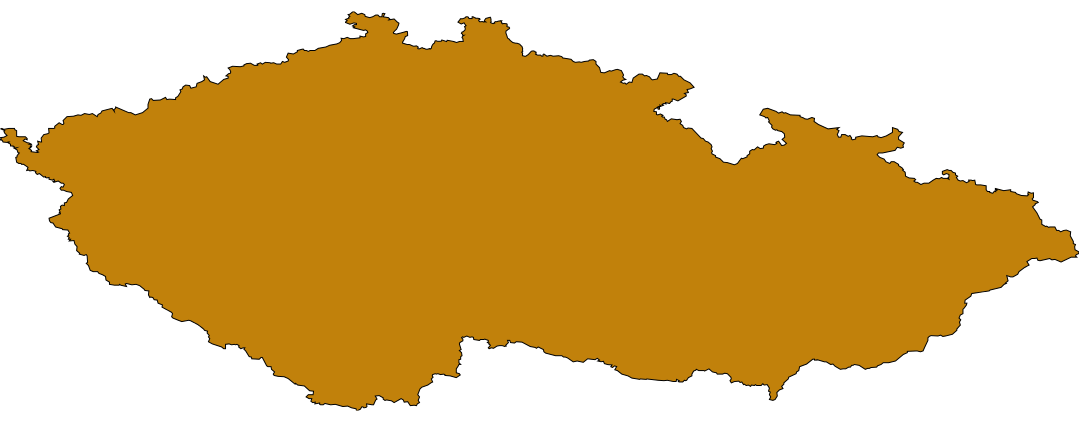
\includegraphics[width=0.5\textwidth]{./img/cr.png}
		\caption[GHF workflow]{\centering Czech Republic map for clipping the Europedataset.}
		\label{map_cz}
	\end{figure} 
	
		Above, in this section, we copied all mandatory data to HDFS. The Europe
		dataset was prepared in cloud using performance VMs
		and loaded to HDFS of cluster. In contrast, Czech boundary map has been
		converted to serialized GeoJSON and copied directly from GRASS GIS DataNodes of
		cluster.
		
		The next step is to prepare table which will store only data within Czech boundary.
	\begin{footnotesize}
		\begin{lstlisting}[style=python]
CREATE EXTERNAL TABLE cr_europe(id BIGINT, lat DOUBLE, lon DOUBLE, time TIMESTAMP)
ROW FORMAT DELIMITED FIELDS TERMINATED BY ',';
		\end{lstlisting}
	\end{footnotesize}
For  analyzing relation between vector features, concretely if polygon A contains feature B, thus Czech Republic contains points is used user defined function \textit{ST\_Contains}
	\begin{footnotesize}
		\begin{lstlisting}[style=python]
create temporary function ST_Contains as 'com.esri.hadoop.hive.ST_Contains';
create temporary function ST_GeomFromGeoJson as 'com.esri.hadoop.hive.ST_GeomFromGeoJson';
		\end{lstlisting}
	\end{footnotesize}
The exported GeoJSON file and its geometry can be constructed as binary geometry
 datatype using \textit{ST\_GeomFromGeoJson} UDF.
	\begin{footnotesize}
		\begin{lstlisting}[style=python]
INSERT OVERWRITE TABLE cr_europe
SELECT europe.id, europe.lat,europe.lon,europe.time
FROM europe 
JOIN cr 
WHERE ST_Contains(ST_GeomFromGeoJSON(cr.geometry), ST_Point(europe.lon, europe.lat)) ;
		\end{lstlisting}
	\end{footnotesize}
And than form hiveserver2 console using hd.hive.execute can be executed query for clipping points.


\newpage
	\section*{Attachment: Europe map aggregation}\label{open_street_agg_all}
	
			\begin{figure}[!htbp]
				\centering
				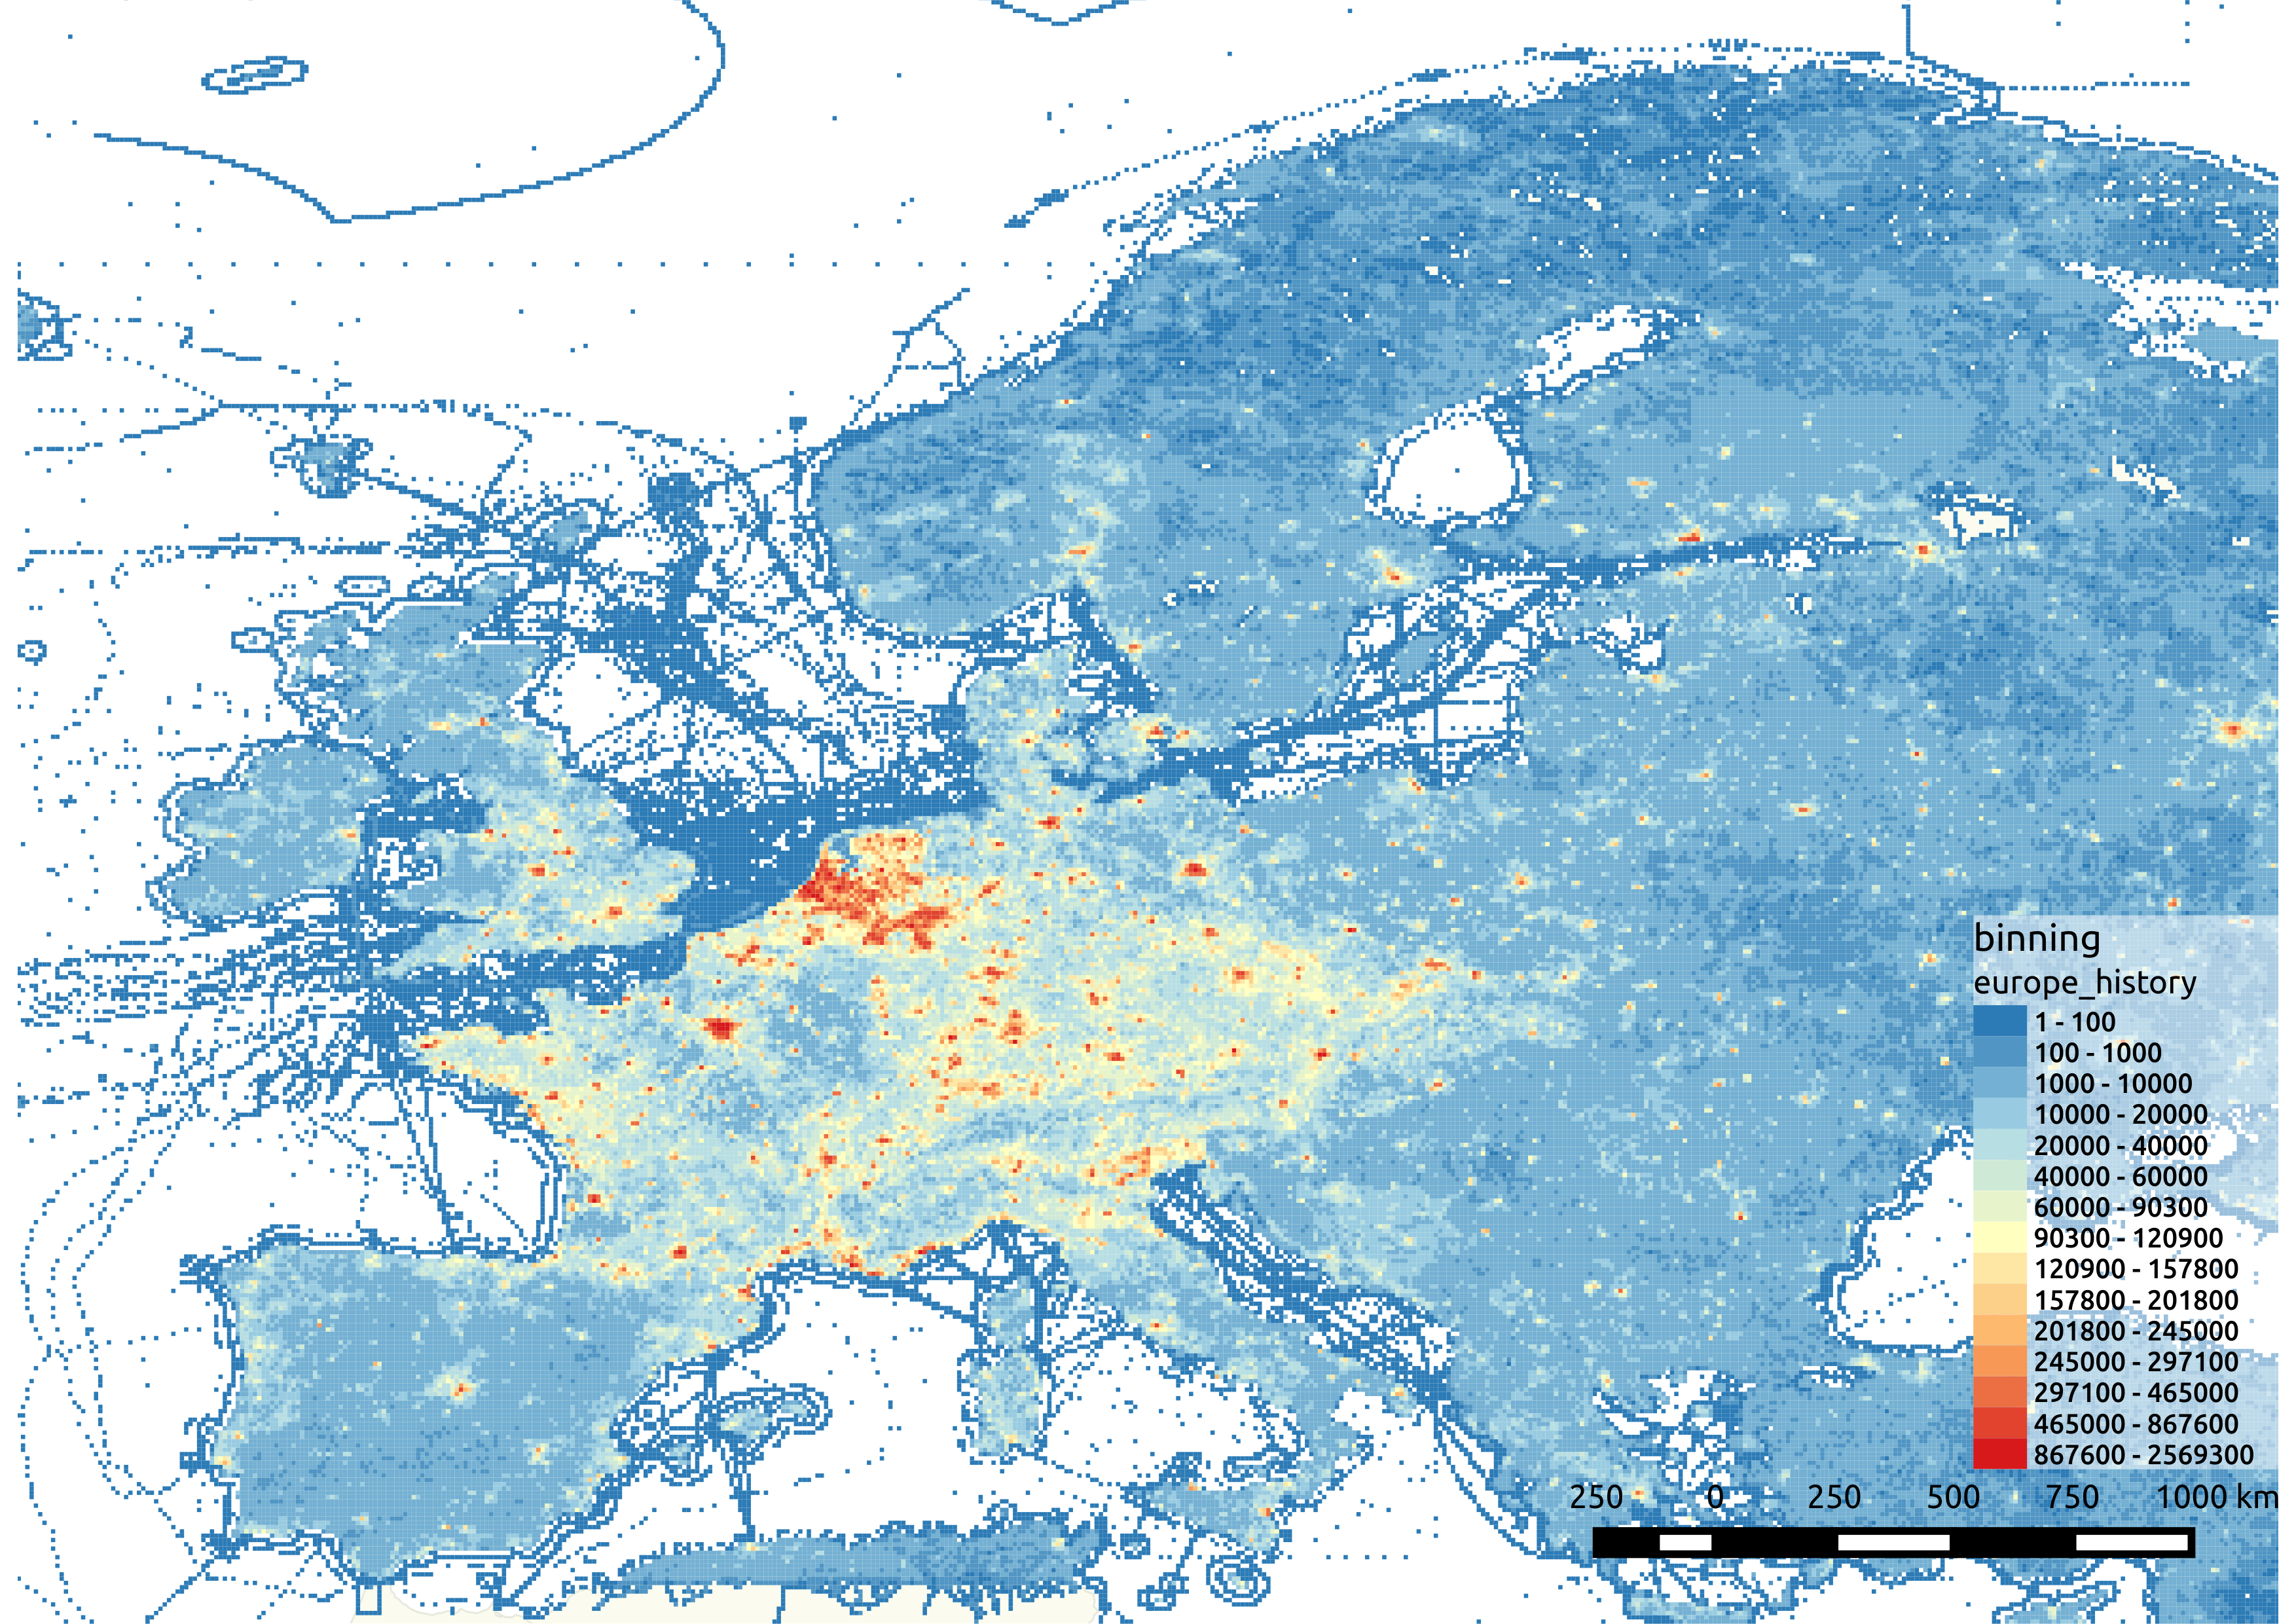
\includegraphics[width=1\textwidth]{./img/osm/history.png}
					\caption[GHF workflow]{\centering Aggregation of OSM points created between 2006 and end of 2014
						The resolution of spatial binning is 0.1 degree (approx 10km). The source OSM map consists of 1.3 billions of points.}
				\label{map_cz}
			\end{figure} 
\newpage		
	\section{Attachment: Configuration of  bdutil and BigQuery migration}\label{pythonscr}
	\begin{footnotesize}
	\begin{lstlisting}[style=mybash]
google_cloud/
|-- bdutil-1.3.4
|   |-- spatial1.sh
|   |-- spatial.sh
|-- bigquery
    `-- mw_schema.json

	\end{lstlisting}
	\end{footnotesize}
	
	
	
	\section{Attachment: Airflow diff}\label{airflow_diff}
	The difference file between Airflow and developed GHF.
\begin{footnotesize}
\begin{lstlisting}[style=mybash]
	.
	|-- src
->	|   -- airflow.dif
	|   `-- grass_hdfs
	|       |-- hdfsgrass
	|       `-- hdfswrapper
	|-- text
	`-- zadani
	
\end{lstlisting}
\end{footnotesize} 	
	\section{Attachment: Source code of GHF}\label{att:install}
	The CD with source code is attached to the printed version of the thesis.
\begin{footnotesize}
\begin{lstlisting}[style=mybash]
.
|-- hdfsgrass
|   |-- grass_map.py
|   |-- hd.db.connect.py
|   |-- hd.esri2map.py
|   |-- hdfs_grass_lib.py
|   |-- hdfs_grass_util.py
|   |-- hd.hdfs.info.py
|   |-- hd.hdfs.in.fs.py
|   |-- hd.hdfs.in.vector.py
|   |-- hd.hdfs.out.vector.py
|   |-- hd.hive.csv.table.py
|   |-- hd.hive.execute.py
|   |-- hd.hive.info.py
|   |-- hd.hive.json.table.py
|   |-- hd.hive.load.py
|   `-- hd.hive.select.py
`-- hdfswrapper
    |-- base_hook.py
    |-- connections.py
    |-- hdfs_hook.py
    |-- hive_hook.py
    |-- hive_table.py
    |-- __init__.py
    |-- security_utils.py
    |-- settings.py
    |-- utils.py
    `-- webhdfs_hook.py

\end{lstlisting}
\end{footnotesize} 
\end{document}








